% -*- Mode:TeX -*-

%% IMPORTANT: The official thesis specifications are available at:
%%            http://libraries.mit.edu/archives/thesis-specs/
%%
%%            Please verify your thesis' formatting and copyright
%%            assignment before submission.  If you notice any
%%            discrepancies between these templates and the 
%%            MIT Libraries' specs, please let us know
%%            by e-mailing thesis@mit.edu

%% The documentclass options along with the pagestyle can be used to generate
%% a technical report, a draft copy, or a regular thesis.  You may need to
%% re-specify the pagestyle after you \include  cover.tex.  For more
%% information, see the first few lines of mitthesis.cls. 

%\documentclass[12pt,vi,twoside]{mitthesis}
%%
%%  If you want your thesis copyright to you instead of MIT, use the
%%  ``vi'' option, as above.
%%
%\documentclass[12pt,twoside,leftblank]{mitthesis}
%%
%% If you want blank pages before new chapters to be labelled ``This
%% Page Intentionally Left Blank'', use the ``leftblank'' option, as
%% above. 

\documentclass[12pt,twoside]{mitthesis}
\usepackage{lgrind}
%% These have been added at the request of the MIT Libraries, because
%% some PDF conversions mess up the ligatures.  -LB, 1/22/2014
\usepackage{cmap}
\usepackage[T1]{fontenc}

\usepackage{amsmath, amssymb, amsthm, mathrsfs, lscape, graphicx, color, enumerate, textcomp, colonequals, fullpage, url, float}
\usepackage[backref]{hyperref}
\usepackage[alphabetic,backrefs,lite]{amsrefs}
\usepackage{harpoon}

\input xy
\xyoption{all}


\makeatletter
\newcommand{\pushright}[1]{\ifmeasuring@#1\else\omit\hfill$\displaystyle#1$\fi\ignorespaces}
\newcommand{\pushleft}[1]{\ifmeasuring@#1\else\omit$\displaystyle#1$\hfill\fi\ignorespaces}
\makeatother


\newtheorem{thm}[subsection]{Theorem}
\newtheorem{conjecture}[subsection]{Conjecture}
\newtheorem*{defn}{Definition}
\newtheorem{corollary}[subsection]{Corollary}
\newtheorem{lemma}[subsection]{Lemma}
\newtheorem{claim}[subsection]{Claim}
\newtheorem{prop}[subsection]{Proposition}
\newtheorem*{lem}{Lemma}
\newtheorem*{fact}{Fact}
\newtheorem*{cor}{Corollary}
\newtheorem*{theo}{Theorem}

\newtheorem{remark}[subsection]{Remark}

\theoremstyle{definition}
\newtheorem{defin}[subsection]{Definition}
\newtheorem{rmk}[subsection]{Remark}

\renewcommand{\labelenumi}{(\alph{enumi})}

\newcommand{\isom}{\cong}
\newcommand{\R}{\mathbb R}
\newcommand{\Q}{\mathbb Q}
\newcommand{\Z}{\mathbb Z}
\newcommand{\N}{\mathbb N}
\newcommand{\C}{\mathbb C}
\renewcommand{\O}{\mathcal{O}}
\newcommand{\A}{\mathbb A}
\newcommand{\F}{\mathbb F}
\renewcommand{\P}{\mathbb P}
\newcommand{\kX}{k[x_1, \dots, x_n]}
\newcommand{\Cl}{{\bf Claim:} }
\renewcommand{\phi}{\varphi}
\newcommand{\p}{\mathfrak{p}}
%\newcommand{\Sch}{\mathfrak{S}\mathrm{ch}}
%\newcommand{\Rg}{\mathfrak{R}\mathrm{ings}}
%\newcommand{\Spec}{\mathrm{Spec}\ }
\newcommand{\mcal}{\mathcal}

\DeclareMathOperator{\Art}{Art}
\DeclareMathOperator{\Gal}{Gal}
\DeclareMathOperator{\Aut}{Aut}
\DeclareMathOperator{\wt}{wt}
\DeclareMathOperator{\Pic}{Pic}
\DeclareMathOperator{\disc}{disc}
\DeclareMathOperator{\cha}{char}
\DeclareMathOperator{\im}{im}
\DeclareMathOperator{\rank}{rank}
\DeclareMathOperator{\lcm}{lcm}
\DeclareMathOperator{\codim}{codim}
\DeclareMathOperator{\Hom}{Hom}
\DeclareMathOperator{\ord}{ord}
\DeclareMathOperator{\Spec}{Spec}
\DeclareMathOperator{\Proj}{Proj}
\DeclareMathOperator{\Tr}{Tr}
\DeclareMathOperator{\sw}{sw}
\DeclareMathOperator{\PGL}{PGL_2}

\renewcommand{\setminus}{-}

\newcommand{\harpoon}{\overset{\rightharpoonup}}

\pagestyle{plain}

%% This bit allows you to either specify only the files which you wish to
%% process, or `all' to process all files which you \include.
%% Krishna Sethuraman (1990).

%\typein [\files]{Enter file names to process, (chap1,chap2 ...), or `all' to
%process all files:}
%\def\all{all}
%\ifx\files\all \typeout{Including all files.} \else \typeout{Including only \files.} \includeonly{\files} \fi

\begin{document}

% -*-latex-*-
% 
% For questions, comments, concerns or complaints:
% thesis@mit.edu
% 
%
% $Log: cover.tex,v $
% Revision 1.8  2008/05/13 15:02:15  jdreed
% Degree month is June, not May.  Added note about prevdegrees.
% Arthur Smith's title updated
%
% Revision 1.7  2001/02/08 18:53:16  boojum
% changed some \newpages to \cleardoublepages
%
% Revision 1.6  1999/10/21 14:49:31  boojum
% changed comment referring to documentstyle
%
% Revision 1.5  1999/10/21 14:39:04  boojum
% *** empty log message ***
%
% Revision 1.4  1997/04/18  17:54:10  othomas
% added page numbers on abstract and cover, and made 1 abstract
% page the default rather than 2.  (anne hunter tells me this
% is the new institute standard.)
%
% Revision 1.4  1997/04/18  17:54:10  othomas
% added page numbers on abstract and cover, and made 1 abstract
% page the default rather than 2.  (anne hunter tells me this
% is the new institute standard.)
%
% Revision 1.3  93/05/17  17:06:29  starflt
% Added acknowledgements section (suggested by tompalka)
% 
% Revision 1.2  92/04/22  13:13:13  epeisach
% Fixes for 1991 course 6 requirements
% Phrase "and to grant others the right to do so" has been added to 
% permission clause
% Second copy of abstract is not counted as separate pages so numbering works
% out
% 
% Revision 1.1  92/04/22  13:08:20  epeisach

% NOTE:
% These templates make an effort to conform to the MIT Thesis specifications,
% however the specifications can change.  We recommend that you verify the
% layout of your title page with your thesis advisor and/or the MIT 
% Libraries before printing your final copy.
\title{Invariants linked to models of curves over discrete valuation rings}

\author{Padmavathi Srinivasan}
% If you wish to list your previous degrees on the cover page, use the 
% previous degrees command:
%       \prevdegrees{A.A., Harvard University (1985)}
% You can use the \\ command to list multiple previous degrees
%       \prevdegrees{B.S., University of California (1978) \\
%                    S.M., Massachusetts Institute of Technology (1981)}
\department{Department of Mathematics}

% If the thesis is for two degrees simultaneously, list them both
% separated by \and like this:
% \degree{Doctor of Philosophy \and Master of Science}
\degree{Doctor of Philosophy}

% As of the 2007-08 academic year, valid degree months are September, 
% February, or June.  The default is June.
\degreemonth{June}
\degreeyear{2016}
\thesisdate{April 29, 2016}

%% By default, the thesis will be copyrighted to MIT.  If you need to copyright
%% the thesis to yourself, just specify the `vi' documentclass option.  If for
%% some reason you want to exactly specify the copyright notice text, you can
%% use the \copyrightnoticetext command.  
%\copyrightnoticetext{\copyright IBM, 1990.  Do not open till Xmas.}

% If there is more than one supervisor, use the \supervisor command
% once for each.
\supervisor{Bjorn Poonen}{Claude Shannon Professor of Mathematics}

% This is the department committee chairman, not the thesis committee
% chairman.  You should replace this with your Department's Committee
% Chairman.
\chairman{Alexei Borodin}{Chairman, Department Committee on Graduate Theses}

% Make the titlepage based on the above information.  If you need
% something special and can't use the standard form, you can specify
% the exact text of the titlepage yourself.  Put it in a titlepage
% environment and leave blank lines where you want vertical space.
% The spaces will be adjusted to fill the entire page.  The dotted
% lines for the signatures are made with the \signature command.
\maketitle

% The abstractpage environment sets up everything on the page except
% the text itself.  The title and other header material are put at the
% top of the page, and the supervisors are listed at the bottom.  A
% new page is begun both before and after.  Of course, an abstract may
% be more than one page itself.  If you need more control over the
% format of the page, you can use the abstract environment, which puts
% the word "Abstract" at the beginning and single spaces its text.

%% You can either \input (*not* \include) your abstract file, or you can put
%% the text of the abstract directly between the \begin{abstractpage} and
%% \end{abstractpage} commands.

% First copy: start a new page, and save the page number.
\cleardoublepage
% Uncomment the next line if you do NOT want a page number on your
% abstract and acknowledgments pages.
% \pagestyle{empty}
\setcounter{savepage}{\thepage}
\begin{abstractpage}
% $Log: abstract.tex,v $
% Revision 1.1  93/05/14  14:56:25  starflt
% Initial revision
% 
% Revision 1.1  90/05/04  10:41:01  lwvanels
% Initial revision
% 
%
%% The text of your abstract and nothing else (other than comments) goes here.
%% It will be single-spaced and the rest of the text that is supposed to go on
%% the abstract page will be generated by the abstractpage environment.  This
%% file should be \input (not \include 'd) from cover.tex.
This thesis consists of two parts. In part one of this thesis, we study the relationship between the Artin conductor and the minimal discriminant of a hyperelliptic curve defined over the fraction field $K$ of a discrete valuation ring. The Artin conductor and the minimal discriminant are two measures of degeneracy of the singular fiber in a family of hyperelliptic curves. In the case of elliptic curves, the Ogg-Saito formula shows that (the negative of) the Artin conductor equals the minimal discriminant. In the case of genus $2$ curves, Liu showed that equality no longer holds in general, but the two invariants are related by an inequality. We extend Liu's inequality to hyperelliptic curves of arbitrary genus, assuming rationality of the Weierstrass points over $K$. 

In part two of this thesis, we compute the sizes of component groups and Tamagawa numbers of N\'{e}ron models of Jacobians using matrix tree theorems from combinatorics. Raynaud gave a description of the component group of the special fiber of the N\'{e}ron model of a Jacobian, in terms of the multiplicities and intersection numbers of components in the special fiber of a regular model of the underlying curve. Bosch and Liu used this description, along with some Galois cohomology computations to provide similar descriptions of Tamagawa numbers. We use various versions of the matrix tree theorem to make Raynaud's and Bosch and Liu's descriptions more explicit in terms of the combinatorics of the dual graph and the action of the absolute Galois group of the residue field on it. We then derive some consequences of these explicit descriptions. First, we use the explicit formula to provide a new geometric condition on the curve for obtaining a uniform bound on the size of the component group of its Jacobian. Then we prove a certain periodicity property of the component group of a Jacobian under contraction of connecting chains of specified lengths in the dual graph. As a third application, we obtain an alternate proof of one of the key steps in Halle and Nicaise's proof of the rationality of the N\'{e}ron component series for Jacobians. 
\end{abstractpage}

% Additional copy: start a new page, and reset the page number.  This way,
% the second copy of the abstract is not counted as separate pages.
% Uncomment the next 6 lines if you need two copies of the abstract
% page.
% \setcounter{page}{\thesavepage}
% \begin{abstractpage}
% % $Log: abstract.tex,v $
% Revision 1.1  93/05/14  14:56:25  starflt
% Initial revision
% 
% Revision 1.1  90/05/04  10:41:01  lwvanels
% Initial revision
% 
%
%% The text of your abstract and nothing else (other than comments) goes here.
%% It will be single-spaced and the rest of the text that is supposed to go on
%% the abstract page will be generated by the abstractpage environment.  This
%% file should be \input (not \include 'd) from cover.tex.
This thesis consists of two parts. In part one of this thesis, we study the relationship between the Artin conductor and the minimal discriminant of a hyperelliptic curve defined over the fraction field $K$ of a discrete valuation ring. The Artin conductor and the minimal discriminant are two measures of degeneracy of the singular fiber in a family of hyperelliptic curves. In the case of elliptic curves, the Ogg-Saito formula shows that (the negative of) the Artin conductor equals the minimal discriminant. In the case of genus $2$ curves, Liu showed that equality no longer holds in general, but the two invariants are related by an inequality. We extend Liu's inequality to hyperelliptic curves of arbitrary genus, assuming rationality of the Weierstrass points over $K$. 

In part two of this thesis, we compute the sizes of component groups and Tamagawa numbers of N\'{e}ron models of Jacobians using matrix tree theorems from combinatorics. Raynaud gave a description of the component group of the special fiber of the N\'{e}ron model of a Jacobian, in terms of the multiplicities and intersection numbers of components in the special fiber of a regular model of the underlying curve. Bosch and Liu used this description, along with some Galois cohomology computations to provide similar descriptions of Tamagawa numbers. We use various versions of the matrix tree theorem to make Raynaud's and Bosch and Liu's descriptions more explicit in terms of the combinatorics of the dual graph and the action of the absolute Galois group of the residue field on it. We then derive some consequences of these explicit descriptions. First, we use the explicit formula to provide a new geometric condition on the curve for obtaining a uniform bound on the size of the component group of its Jacobian. Then we prove a certain periodicity property of the component group of a Jacobian under contraction of connecting chains of specified lengths in the dual graph. As a third application, we obtain an alternate proof of one of the key steps in Halle and Nicaise's proof of the rationality of the N\'{e}ron component series for Jacobians. 
% \end{abstractpage}

\cleardoublepage

\section*{Acknowledgments}



%%%%%%%%%%%%%%%%%%%%%%%%%%%%%%%%%%%%%%%%%%%%%%%%%%%%%%%%%%%%%%%%%%%%%%
% -*-latex-*-

% Some departments (e.g. 5) require an additional signature page.  See
% signature.tex for more information and uncomment the following line if
% applicable.
% % -*- Mode:TeX -*-
%
% Some departments (e.g. Chemistry) require an additional cover page
% with signatures of the thesis committee.  Please check with your
% thesis advisor or other appropriate person to determine if such a 
% page is required for your thesis.  
%
% If you choose not to use the "titlepage" environment, a \newpage
% commands, and several \vspace{\fill} commands may be necessary to
% achieve the required spacing.  The \signature command is defined in
% the "mitthesis" class
%
% The following sample appears courtesy of Ben Kaduk <kaduk@mit.edu> and
% was used in his June 2012 doctoral thesis in Chemistry. 

\begin{titlepage}
\begin{large}
This doctoral thesis has been examined by a Committee of the Department
of Chemistry as follows:

\signature{Professor Jianshu Cao}{Chairman, Thesis Committee \\
   Professor of Chemistry}

\signature{Professor Troy Van Voorhis}{Thesis Supervisor \\
   Associate Professor of Chemistry}

\signature{Professor Robert W. Field}{Member, Thesis Committee \\
   Haslam and Dewey Professor of Chemistry}
\end{large}
\end{titlepage}


\pagestyle{plain}
  % -*- Mode:TeX -*-
%% This file simply contains the commands that actually generate the table of
%% contents and lists of figures and tables.  You can omit any or all of
%% these files by simply taking out the appropriate command.  For more
%% information on these files, see appendix C.3.3 of the LaTeX manual. 
\tableofcontents
%\newpage
%\listoffigures
%\newpage
%\listoftables


%% This is an example first chapter.  You should put chapter/appendix that you
%% write into a separate file, and add a line \include{yourfilename} to
%% main.tex, where `yourfilename.tex' is the name of the chapter/appendix file.
%% You can process specific files by typing their names in at the 
%% \files=
%% prompt when you run the file main.tex through LaTeX.
\chapter{Introduction}
Let $R$ be a discrete valuation ring with fraction field $K$ and residue field $k$. Let $X$ be a {\color{blue}{\textsf{nice}}} (smooth, projective and geometrically integral) $K$-variety. The variety $X$ is said to have {\color{blue}{\textsf{good reduction}}} if there exists a smooth and proper $R$-scheme $\mathscr{X}$ whose generic fiber $\mathscr{X}_K$ is isomorphic to $X$. In his 1967 paper \cite{ogg}, Ogg proved that an elliptic curve $E$ (a nice group variety of dimension $1$) defined over $K$ has good reduction if and only if the natural action of the inertia group $I_K$ on the $\ell$-adic Tate module of $E$ is trivial. This criterion (the {\textit{N\'{e}ron--Ogg--Shafarevich criterion}}) was later generalized by Serre and Tate \cite{serretate} to abelian varieties of arbitrary dimension. The nontriviality of the inertia action on the Tate module of an abelian variety is captured by the nonvanishing of a certain numerical invariant, called (the exponent of) the {\color{blue}{\textsf{conductor}}} of the abelian variety (see Section~\ref{defcond} for the definition). For an abelian variety defined over a number field, the local conductors at various primes appear in the conjectured functional equation for the $L$-function of the abelian variety.

Elliptic curves occupy a special place in the study of nice varieties, since they straddle the worlds of algebraic curves (nice varieties of dimension $1$) and abelian varieties (nice group varieties). One can ask if the N\'{e}ron-Ogg-Shafarevich criterion extends to curves of arbitrary genus, with $H^1(X_{\overline{K}},\Q_{\ell})$ in place of the the $\ell$-adic Tate module, but this turns out to be false \cite[Theorem~3.2]{oda} {\footnote{For an explicit example, see {\tt{\url{http://mathoverflow.net/questions/91909/a-curve-with-bad-reduction-for-which-the-jacobian-has-good-reduction}}}.}}.
% {\footnote{Let $E$ be an elliptic curve over $\Q_2$ such that $E$ has good reduction. Then the inertia action on $H^1(E_{\overline{\Q_2}},\Q_l)$ is trivial. Let $C$ be a nontrivial $E$-torsor. Then $C$ cannot have good reduction, since (i) the Hasse-Weil bounds imply that every smooth genus $1$ curve over $\F_2$ has a rational point, and, (ii) the valuative criterion for properness implies that any smooth $\F_2$-point on the reduction lifts to a smooth $\Q_2$-point on $C$. However, the $\Gal (\overline{\Q_2}/\Q_2)$-modules $H^1(E_{\overline{\Q_2}},\Q_l)$ and $H^1(C_{\overline{\Q_2}},\Q_l)$ are isomorphic. See \cite[Theorem~3.2]{oda} for an anabelian generalization of the N\'{e}ron-Ogg-Shafarevich criterion.}}
The correct generalization of the conductor also takes into account the dimensions of the cohomology groups of the special fiber of the minimal proper regular model of the algebraic curve, and this is encoded in another numerical invariant called the {\color{blue}{\textsf{Artin conductor}}} (see Section~\ref{defcond} for the definition). For curves of genus $g \geq 2$, the Artin conductor vanishes exactly when the minimal proper regular model of the curve is smooth over $R$. For a nice curve defined over a number field, the Artin conductors at various primes appear in the conjectured functional equation for the $L$-function associated to a global proper regular model of $X$ over the ring of integers of the number field \cite[Proposition 1.1]{bloch}. The (negative of the) Artin conductor is an upper bound for the conductor of the $I_K$-representation $H^1(X_{\overline{K}},\Q_{\ell})$, and the difference of the two conductors is one less than the number of the components in the special fiber of the minimal proper regular model of $X$ (Lemma~\ref{artcondfor}).

Elliptic curves over $K$ also have integral Weierstrass equations over $R$. An {\color{blue}{\textsf{integral Weierstrass equation}}} is an equation of the form 
\[ F(x,y,z) = y^2z+a_1xyz+a_3yz^2+x^3+a_2x^2z+a_4xz^2+a_6z^3 \]
that cuts out the elliptic curve in $\P^2_K$, with $\{a_1,a_2,\ldots,a_6\} \subset R$. 
% {\color{red}{We work with more general(even degree) integral Weierstrass equations for most of the paper --- should we give the definition that we use here (which might be confusing) or omit it altogether and refer to the Definitions section? Proposition 8(c) in \cite{liuminmod} explains why the two are equal... We could also make it a remark in the definitions section, after giving the more general definition for hyperelliptic curves.}} 
Any such equation has an associated (valuation of) {\color{blue}{\textsf{discriminant}}}{\footnote{For an elliptic curve over a global field, one can also define a global conductor and a global discriminant; our definitions of the discriminant and the conductor equal the valuation of the global discriminant and conductor; the definitions that we use are better suited to our situation since we are interested in studying the local behaviour at a {\textit{single}} prime.}} \cite[p.42, Section III.1]{babysil}, which is a nonnegative integer that measures how far the corresponding closed subscheme of $\P^2_R$ is from being smooth over $R$. An integral Weierstrass equation that minimizes the value of the discriminant is called a {\color{blue}{\textsf{minimal Weierstrass equation}}}, and the corresponding discriminant is called the {\color{blue}{\textsf{minimal discriminant}}}. It can be shown that an elliptic curve over $K$ has good reduction if and only if it has an integral Weierstrass equation with discriminant $0$ (Proposition~\ref{goodreddisccrit}\textup{(c)}). 

Since elliptic curves have these two measures of failure of good reduction, namely the Artin conductor and the minimal discriminant, it is quite natural to ask how these two invariants are related. In \cite{ogg}, Ogg showed that the minimal discriminant of an elliptic curve over $K$ equals the (negative) of the Artin conductor. He attributes this to a result of Tate from 1960 in the case when $\cha k \neq 2,3$, and remarks that the results in his paper are essentially about filling in the two remaining cases. However, the arguments in his paper fall short of handling the mixed characteristic $2$ case, i.e., when $\cha K = 0$ and $\cha k = 2$. The gap in his proof was finally filled in 20 years later by Saito in \cite{saito2}. The proof given by Ogg proceeds by a lengthy case by case analysis, and uses the Kodaira-N\'{e}ron classification of the possible special fibers of proper regular models of elliptic curves. 
%{\color{red}{Why does it fail in mixed char 2? Has something to do with Newton's method of solving polynomial equations...}} 
Saito's result, on the other hand, is far more general, and holds for proper regular models of {\textit{arbitrary}} curves, not just elliptic curves. 

To describe Saito's result, we first need to recall some earlier results of Mumford and Deligne. For any integer $g \geq 1$, let $\overline{\mathcal{M}}_g$ be the Deligne-Mumford compactification of the moduli space of smooth genus $g$ curves. In \cite[Theorem~5.10]{mumford}, Mumford established relations between certain natural classes of line bundles in $\Pic \overline{\mathcal{M}}_g$. Deligne used one of Mumford's relations as a template for defining a discriminant for an arbitrary proper regular model $\mathscr{X}$ over $\Spec R$ (see Section~\ref{defdeldisc} for the definition). Saito proved that the (negative of) the Artin conductor of a proper regular model $\mathscr{X}$ equals the discriminant that Deligne defined. This new discriminant, which we call the {\color{blue}{\textsf{Deligne discriminant}}}, coincides with the minimal discriminant in the case when $\mathscr{X}$ is the minimal proper regular model of an elliptic curve. In the case of genus $2$ curves, Saito relates his result to an explicit formula given by Ueno for the Deligne discriminant when $\cha k = 0$ or when $\cha k > 6$. Ueno's formula is in terms of yet another notion of discriminant that is special to genus $2$ curves, and it uses data pertaining to the geometry of the special fiber of a minimal proper regular model for a genus $2$ curve \cite{ueno}. The explicit classification that Ueno used for special fibers of proper regular models of genus $2$ curves already has over $120$ different types! For higher genus curves, the Deligne discriminant is very hard to explicitly compute in practice.

For a genus $g$ hyperelliptic curve, Liu defined a minimal discriminant that is analogous to the minimal discriminant for elliptic curves (see Section~\ref{mindisdef} for the definition). In \cite{liup}, Liu proved that for a genus $2$ hyperelliptic curve, the minimal discriminant is an upper bound for the (negative of the) Artin conductor. For genus $2$ curves, unlike elliptic curves, the minimal discriminant and the (negative of the) Artin conductor are sometimes different. In his paper, Liu gives an exact formula for the difference. When $\cha k \neq 2$, this difference can be computed quite explicitly in terms of the aforementioned classification of fibers of genus $2$ curves. When the hyperelliptic curve has semistable reduction over $K$, Kausz \cite{kausz} (when $\cha k \neq 2$) and Maugeais \cite{maugeais} (for all residue characteristics) prove theorems that relate the Deligne discriminant to yet another discriminant. We are not sure if Liu's minimal discriminant coincides with the discriminant that is used by Kausz and Maugeais. One of the main results in this thesis is the following.

\begin{thm}\label{main}
 Let $R$ be a discrete valuation ring with perfect residue field $k$. Assume that $\cha k \neq 2$. Let $K$ be the fraction field of $R$. Let $K^{\mathrm{sh}}$ denote the fraction field of the strict henselization of $R$. Let $C$ be a hyperelliptic curve over $K$ of genus $g$. Let $\nu \colon K \rightarrow \Z \cup \{\infty\}$ be the discrete valuation on $K$. Assume that the Weierstrass points of $C$ are $K^{\mathrm{sh}}$-rational. Let $S = \Spec R$ and let $\mathcal{X} \rightarrow S$ be the minimal proper regular model of $C$. Let $\nu(\Delta)$ denote the minimal discriminant of $C$. Then
 \[ -\Art (\mathcal{X}/S) \leq \nu(\Delta) .\]
\end{thm}

Our method of proof is different from Liu's method for genus $2$ curves. Liu compares the Deligne discriminant of the minimal proper regular model and the minimal discriminant by comparing both of them to a third  discriminant that he defines, following a definition given by Ueno \cite[Definition~1, Th\'{e}or\`{e}me~1 and Th\'{e}or\`{e}me~2]{liup}. This third discriminant is specific to genus $2$ curves.

We instead proceed by constructing an explicit proper regular model for $C$ (Section~\ref{construct}). We can immediately reduce to the case where $R$ is a henselian discrete valuation ring with algebraically closed residue field. We may then choose a minimal Weierstrass equation of the form, $y^2-f(x)$ where $f$ is a monic polynomial in $R[x]$ that splits completely. If the Weierstrass points of $C$ specialize to distinct points of the special fiber, then the polynomial $y^2-f(x)$, suitably homogenized, defines a smooth proper model of $C$ in a weighted projective space over $R$ (see Section~\ref{mindisdef} for the definition). If not, we iteratively blow up $\P^1_R$ until the Weierstrass points have distinct specializations. After a few additional blow-ups, we take the normalization of the resulting scheme in the function field of $C$. This gives us a (not necessarily minimal) proper regular model for $C$ (Theorem~\ref{Xisregular}). 

We have the relation $-\Art(X/S) = n(X_s)-1+\tilde{f}$ for a proper regular model $X$ of $C$, where $n(X_s)$ is the number of components of the special fiber of $X$ and $\tilde{f}$ is an integer that depends only on $C$ and not on the particular proper regular model chosen. This tells us that to bound $-\Art (X/S)$ for the minimal proper regular model from above, it suffices to bound $-\Art (X/S)$ for some proper regular model for the curve.

In Section~\ref{explicitformula}, we give an explicit formula for the Deligne discriminant for the model we have constructed. After a brief interlude on dual graphs in Section~\ref{dualgraphs}, we restate the formula for the Deligne discriminant using dual graphs. This formula tells us that the Deligne discriminant decomposes as a sum of terms, indexed by the vertices of the dual graph of the special fiber of the proper regular model we constructed (Section~\ref{DDanddual}). In Section~\ref{description}, we give a description of the rest of the strategy to prove the main theorem using this formula. The additional ingredients that are necessary are a decomposition of the minimal discriminant into a sum of terms depending on the local geometry of the graph (Section~\ref{breakupnaive}) and explicit formulae for the local terms in the Deligne discriminant in terms of dual graphs (Section~\ref{localcontribution}). In Section~\ref{comparison}, we show how to compare the Deligne discriminant and the minimal discriminant locally. To finish the proof, we sum the local inequalities to obtain $-\Art(X/S) \leq \nu(\Delta)$. 

One application of Theorem~\ref{main} is to give upper bounds on the number of components in the special fiber of the minimal proper regular model (Corollary~\ref{number}). This has applications to Chabauty's method of finding rational points on curves of genus at least $2$ \cite{poonenstoll}. 

It might be possible to adapt the same strategy to extend Theorem~\ref{main} to the case of nonrational Weierstrass points. The main difficulties in making this approach work are in understanding the right analogues of the results in Sections~\ref{breakupnaive} and \ref{localcontribution}.

In the second half of this thesis, we study the component group scheme attached to the special fiber of the N\'{e}ron model of a Jacobian. The N\'{e}ron model of an abelian variety $A$ defined over $K$ is in a certain sense the best possible extension of $A$ to a smooth, commutative group scheme $\mathcal{A}$ over $R$ (See Section~\ref{defneron} for a precise definition). The N\'{e}ron model $\mathcal{A}$ is proper over $S$ if and only if the abelian variety has good reduction. In general, the special fiber of the N\'{e}ron model might not be proper, or even connected. The special fiber of the N\'{e}ron model $\mathcal{A}_s$ fits in an exact sequence 
\[ 0 \rightarrow \mathcal{A}_s^0 \rightarrow \mathcal{A}_s \rightarrow \Phi \rightarrow 0,  \]
where $\mathcal{A}_s^0$ is a connected group scheme and $\Phi$ is a finite \'{e}tale group scheme, called the {\color{blue}{\textsf{component group scheme}}}. Let $\overline{k}$ be an algebraic closure of $k$. The {\color{blue}{\textsf{component group}}} is $\Phi(\overline{k})$, and the {\color{blue}{\textsf{Tamagawa number}}} is the order of the group $\Phi(k)$. 

Computing the orders of component groups and Tamagawa numbers have arithmetic applications. For an abelian variety $A$ over a number field $K$, bounds on the order of the component group at a prime is one of the inputs for giving bounds on the order of the torsion subgroup of $A(K)$. Mazur used this fact in his paper \cite{mazur} to prove that for an elliptic curve $E$ over $\Q$, the order of the torsion subgroup of $E(\Q)$ is bounded above by $16$. The local Tamagawa numbers appear in the statement of the full Birch and Swinnerton-Dyer conjecture; explicit verification of the full BSD conjecture for a specific abelian variety requires explicit computation of Tamagawa numbers. 

In the special case where the abelian variety is the Jacobian $J$ of a nice $K$-curve $X$, there are multiple approaches for constructing the N\'{e}ron model. Under relatively mild hypotheses, one can construct the N\'{e}ron model of $J$ by using the theory of the relative Picard scheme of a proper regular model of $X$ over $\Spec R$ \cite[Chapter~9, Section~5, Theorem~4]{blr}. This method also leads to a description of the component group of the special fiber of the N\'{e}ron model \cite[Chapter 9, Section 6, Theorem 1]{blr}: the component group is the middle homology group of a three term complex of free abelian groups, where the maps between the groups in the complex are given in terms of multiplicities and intersection numbers of the components in the special fiber of a proper regular model of $X \times K^{\textup{sh}}$ (see Section~\ref{defcompgrp} for details). The free abelian groups in this complex also admit natural actions of the absolute Galois group $G$ of $k$ that commute with the maps in the complex; Bosch and Liu used this action to give a description of $\Phi(k)$ similar to the description of the component group (Theorem~\ref{galcoh}), assuming that $G$ is procyclic.

The multiplicities and the intersection numbers of components in the special fiber of a proper regular model can be encoded in a weighted graph, called the {\color{blue}{\textsf{dual graph}}} of the special fiber (See Section~\ref{weightdualgraph} for the definition). In Theorem~\ref{compformula}, we give an explicit formula for the order of the component group that can be expressed in terms of the combinatorics of this dual graph, using the matrix-tree theorem (\ref{matrixtreeforgraphs}). Formulas of this type for the component group are not new, and special cases are well-known; when the proper regular model is semistable, the order of the component group equals the number of spanning trees in the dual graph, and when the dual graph is a tree, the order of the component group equals the product of the multiplicities of the components raised to certain exponents; each exponent depends on the number of neighbours of the corresponding vertex in the dual graph. The formula in Theorem~\ref{compformula} can be viewed as a hybrid of the formula in these two special cases, where each spanning tree in the dual graph is assigned a weight, and the expression for the weight is formally similar to the expression for the order of the component group in the case when the dual graph is a tree. A version of this formula is implicit in the proof of \cite[Corollary~3.5]{lor1}. Using a weighted version of the matrix-tree theorem (Theorem~\ref{matrixtree}), we obtain a similar formula for Tamagawa numbers expressed in terms of the combinatorics of a certain quotient graph.

For an elliptic curve having good or additive reduction the order of the component group is atmost $4$. Using our explicit formula in Theorem~\ref{compformula}, we prove an analogue of this fact for curves of higher genus (Theorem~\ref{uniformbound}). The condition of having good or additive reduction in genus $1$ is replaced by a certain geometric condition on the $-2$ curves in the minimal proper regular model in higher genus. To explain the nature of this geometric condition, we first recall that any connected commutative algebraic group over a perfect field admits a three step filtration, where the quotients are an abelian variety, a torus, and a unipotent group. The dimensions of the corresponding groups for the special fiber $\mathcal{A}_s^0$ of the N\'{e}ron model of any abelian variety, are called the abelian rank, toric rank and unipotent rank respectively. The condition of having good or additive reduction for an elliptic curve is equivalent to the elliptic curve having toric rank $0$. When the abelian variety is a Jacobian, the unipotent, abelian and toric ranks can be computed from the geometry of the special fiber of a proper regular model of the curve \cite[p.148]{lor}. The toric rank equals the first Betti number of the dual graph of the special fiber of a proper regular model. In \cite{lor}, Lorenzini shows that there is a uniform bound on the order of component groups of Jacobians having toric rank $0$. The condition that we impose is strictly weaker than requiring that $A$ have toric rank $0$, since we only disallow cycles of $-2$ curves, and not cycles of curves where at least one of the curves in the cycle has geometric genus $\geq 1$. 

Even though the order of the component group for a Jacobian is well-understood, the structure of the group remains quite mysterious. There are very few cases where the group structure is explicitly known; the only exceptions are genus $1$ curves where one can use the Kodaira-N\'{e}ron classification and a certain subset of Jacobians having potentially good reduction as described in \cite[Theorem~2.1]{lorpotgood} .
% Inspired by the explicit formula in Theorem~\ref{compformula} and the explicit calculations of component groups for elliptic curves for the various Kodaira-N\'{e}ron types, 
We prove a periodicity property of the component group under partial contraction of connecting chains (Theorem~\ref{compcontract}), generalizing \cite[Corollary~4.7]{bano} from the case of unweighted graphs. 

The formation of the N\'{e}ron model of an abelian variety does not commute with ramified base change: if $(R',K')$ is a ramified extension of $(R,K)$, the N\'{e}ron model of $A \times_K K'$ might not be equal to $\mathcal{A} \times_R R'$. The {\color{blue}{\textsf{N\'{e}ron component series}}} defined by Halle and Nicaise (see Section~\ref{defcompser} for the definition) simultaneously records the changes in the order of the component group under all tamely ramified extensions of the base in a power series. This power series is known to be rational in the following three cases: (i) when $A$ acquires semistable reduction after a tame extension of the base, (ii) when the toric rank equals the dimension of $A$ after a base extension, and (iii) when $A$ is a Jacobian. It is believed to be rational in general. Using our explicit formula (Theorem~\ref{compformula}), we provide an alternate proof of the key step in Halle and Nicaise's proof in case (iii), without having to resort to a reduction to the mixed characteristic case (Theorem~\ref{newproof}).




%% This is an example first chapter.  You should put chapter/appendix that you
%% write into a separate file, and add a line \include{yourfilename} to
%% main.tex, where `yourfilename.tex' is the name of the chapter/appendix file.
%% You can process specific files by typing their names in at the 
%% \files=
%% prompt when you run the file main.tex through LaTeX.
\chapter{Background and Definitions}\label{chapdef}
Let $R$ be a henselian discrete valuation ring with algebraically closed residue field $k$. Let $p = \cha k \geq 0$. (The hypotheses on $R$ and $k$ hold for the rest of this thesis, unless explicitly stated otherwise.) Let $K$ be the fraction field of $R$. Let $\overline{K}$ denote a separable closure of $K$. Let $\nu \colon K \rightarrow \Z \cup \{\infty\}$ denote the discrete valuation on $K$. A {\color{blue}{\textsf{$K$-variety}}} is a separated scheme of finite type over $K$. A {\color{blue}{\textsf{nice $K$-curve}}} $C$ is a smooth, projective, geometrically integral $K$-variety of dimension $1$. Let $S = \Spec R$. In this thesis, a {\color{blue}{\textsf{hyperelliptic curve}}} defined over $K$ will be a nice positive-genus $K$-curve which admits a degree $2$ map to $\P^1$ that is defined over $K$. 

\begin{rmk}
 The most general definition for a hyperelliptic curve would be a nice $K$-curve $X$ that admits a degree $2$ map $X \rightarrow C$, where $C$ is a nice genus $0$ curve (that may or may not have rational points). However, we restrict our attention to those hyperelliptic curves for which $C$ has a $K$-point.
\end{rmk}

\section{Weierstrass models and minimal discriminants}\label{defmindisc}
Let $A$ be a commutative ring. Let $g$ be a positive integer $\geq 1$. Let $A[x,y,z]$ be the weighted polynomial ring over $A$  which assigns weight $1$ to the variables $x$ and $z$, and weight $g+1$ to the variable $y$. Let $\P_A = \Proj A[x,y,z]$. Given a polynomial $f(x,y) \in A[x,y]$, its {\color{blue}{\textsf{homogenization}}} $F(x,y,z)$ is given by $F(x,y,z) = z^{\deg f} f(x/z,y/z^{g+1})$, where $\deg f$ is the degree of $f$ in the weighted polynomial ring $A[x,y,z]$.

\begin{defin}
 An {\color{blue}{\textsf{integral Weierstrass equation}}} for a hyperelliptic $K$-curve $C$ of genus $g$ is an equation $f(x,y) = y^2+q(x)y-p(x) = 0$, where $q(x) \in R[x]$ is of degree $\leq g+1$ and $p(x) \in R[x]$ is of degree $\leq 2g+2$, such that the locus cut out by the homogenization of $f$ in $\P_K$ is isomorphic to $C$.
\end{defin}

 Let $A = \Z[p_0,p_1,\ldots,p_{2g+2},q_0,q_1,\ldots,q_{g+1}]$ and let $B = \Spec A$. Let $P(x,z) = \sum_{i=0}^{2g+2}p_ix^iz^{2g+2-i}$ and let $Q(x,z) = \sum_{i=0}^{g+1}q_ix^iz^{g+1-i}$. Let $F(x,y,z)=y^2+Q(x,z)y-P(x,z)$. The universal family of hyperelliptic curves in Weierstrass form $\pi \colon \mathscr{W} \rightarrow B$ is the hypersurface cut out by $F$ in $\P_A$. Standard arguments show that the image (under $\pi$) of the non-smooth locus of $\pi$ is a closed irreducible hypersurface in $B$, and hence is cut out by a single polynomial $\Delta \in A$, determined uniquely up to sign. Over $B \times_{\Z} \Z[1/2]$, this hypersurface is the vanishing locus of the polynomial $\Delta' \colonequals \disc (4P(x,z)+Q(x,z)^2)$. Hence $\Delta = u \Delta'$ for some unit $u$ in $A[1/2]$, i.e., $u = 2^a$ for some $a \in \Z$. To compute $a$, we can use the fact $\Delta$ is a $2$-adic unit when evaluated at any hyperelliptic curve over $\Z$ that has good reduction at $2$ (for example, the hyperelliptic curve given by 
$y^2 + z^{g+1} y = x^{2g+1} z$); this yields $a = -4(g+1)$.

\begin{defin}
 The {\color{blue}{\textsf{discriminant of the hyperelliptic equation}}} $\colon f(x,y) = y^2+q(x)y-p(x) = 0$ equals $\nu(\Delta(f))$, where $\Delta(f)$ equals $\Delta$ evaluated at the coefficients of the homogenization of $f$.
\end{defin}

\begin{defin}\label{mindisdef}\cite[Definition~3, Remarque~4]{liuminmod}
 A {\color{blue}{\textsf{minimal Weierstrass equation}}} for a hyperelliptic $K$-curve $C$ is an integral Weierstrass equation for $C$ whose discriminant is minimal amongst all integral Weierstrass equations of $C$. The discriminant of a minimal Weierstrass equation is called the {\color{blue}{\textsf{minimal discriminant}}}.
\end{defin}

\begin{prop}\label{algo}
 Let $C$ be a hyperelliptic $K$-curve of genus $g$. 
 \begin{enumerate}[\upshape(a)]
  \item The curve $C$ has an integral Weierstrass equation.  
%   \item There exists an algorithm that given a Weierstrass equation defining a hyperelliptic curve $C$ over $K$, computes a minimal Weierstrass equation and the minimal discriminant of $C$. 
  \item If the degree $2$ morphism $C \rightarrow \P^1_K$ has a $K$-rational branch point, then we can find a minimal Weierstrass equation of the form $y^2+q(x)y=p(x)$, where $\deg q \leq g$ and $\deg p \leq 2g+1$. 
  \item If $\cha k \neq 2$, the curve $C$ has a minimal Weierstrass equation of the form $y^2=p(x)$.
 \end{enumerate} 
\end{prop}
\begin{proof} \hfill
\begin{enumerate}
\item We first prove that there exists an integral Weierstrass equation for $C$. Let $\pi \colon C \rightarrow \P^1_K$ be the canonical morphism. Let $D = \pi^*((\infty))$. Using the Riemann-Roch theorem and the fact that $C$ is hyperelliptic, we can pick elements $x,y \in K(C)$ such that $\{1,x\}$ is a basis for $H^0(C,D)$ and $\{1,x,\ldots,x^{g+1},y\}$ is a basis for $H^0(C,(g+1)D)$. Since 
 \begin{itemize}
  \item $\{1,x,\ldots,x^{2g+1},y,yx,\ldots,yx^{g}\}$ is a basis for $H^0(C,(2g+1)D)$, 
  \item $\{1,x,\ldots,x^{2g+2},y,yx,\ldots,yx^{g+1},y^2\}$ span $H^0(C,(2g+2)D)$,
  \item $\dim H^0(C,(2g+2)D) = 3g+5$, and,
  \item $y \notin K(x) \cap H^0(C,(g+1)D)$,
 \end{itemize}
there has to be a nontrivial relation 
 \[y^2+(b_0x^{g+1}+b_1x^g+\ldots+b_{g+1})y = a_0x^{2g+2}+a_1x^{2g+1}+\ldots+a_{2g+2} \]
 for some set $\{b_0,b_1,\ldots,b_{g+1},a_0,a_1,a_{2g+2}\} \subset K$. Replacing $x$ by $u x$ replaces $b_0$ by $u^{g+1}b_0$ and $a_0$ by $u^{2g+2}a_0$, so by making $u$ sufficiently divisible by the uniformizer, we get a nontrivial relation where $b_0,a_0 \in R$. Now if we simultaneously replace $x$ by $u^{-1}x$ and $y$ by $u^{-(g+1)}y$, we get a relation where each $b_i$ is replaced by $u^ib_i$ and each $a_i$ is replaced by $u^ia_i$. By making $u$ sufficiently divisible by the uniformizer of $R$, we can make all the $b_i$ and all the $a_i$ integral. Let $C'$ be the $K$-curve defined by the corresponding weighted homogeneous equation. The complete linear system $H^0(C,(2g+2)D)$ induces a rational map $C \dashrightarrow C'$ that factors via the normalization $\overline{C'}$ of $C'$. The curve $C'$ has arithmetic genus $g(C)$. Therefore the genus of $\overline{C'}$ is less than or equal to $g(C)$, and equality holds only when $C'$ is smooth. Since $C$ and $\overline{C'}$ are both smooth, projective curves, the rational map $C \dashrightarrow \overline{C'}$ is in fact a morphism. Since there are no morphisms from $C$ to a curve of strictly smaller genus, it follows from the Riemann-Hurwitz formula that $C'$ is smooth, and the morphism $C \rightarrow C'$ is an isomorphism. This gives us an integral Weierstrass equation. 
%  \item 
%  The map $C \rightarrow \P^1$ given by the rational function $x$ agrees with the map $\pi$ up to a change of coordinates on $\P^1_K$ that leaves the point $\infty$ fixed. For a fixed divisor $D$, any other Weierstrass equation that has $\pi^*((\infty)) = D$ is given by a change of coordinates that replaces $x$ by $ux+r$ and $y$ by $u^{g+1}y+s(x)$, for some $s(x) \in K[x]$ of degree $\leq g+1$. One can check that this operation subtracts $(4g+4) \nu(u)$ from the discriminant of the original integral Weierstrass equation; in particular, the new discriminant is independent of $s(x)$. This tells us that if we are interested in computing the minimal discriminant, we can restrict our attention to those changes of coordinates on $C$ that arise from a change of coordinates on the underlying $\P^1_K$.
%  
%  In order to give an algorithm that computes the minimal discriminant, it therefore suffices to understand how conjugation by $\PGL(K)$ affects the order of vanishing of the resultant of a pair of homogeneous polynomials $[F(x,z):G(x,z)]$ (in our case $F = 2^{-4(g+1)} \disc (4P(x,z)+Q(x,z)^2)$ and $G$ equals the derivative of $f$ homogenized to a degree $2g+2$ polynomial). In \cite[Theorem~0.1]{rumely}, Rumely explains how this $\PGL(K)$ conjugation action on the valuation of the resultant can be viewed as an action on the type $II$ points of the Berkovich projective line. In fact, he proves that this action gives rise to a continuous function $\P^1_{\textup{Berk}} \rightarrow [0,\infty]$, that is piecewise linear and {\textit{convex upwards}} on each finite line segment of $\P^1_{\textup{Berk}}$. The fact that this function is convex upwards on each finite line segment allows us to search for the minimum discriminant over any field $K$ with finite residue field by a `steepest descent' algorithm on the Bruhat-Tits tree over $K$ (i.e. starting at any point on the Bruhat-Tits tree, we move in a direction that decreases the discriminant until we reach a local minimum) --- this is explained in detail in \cite[Algorithm~B]{rumely}. Since the function is convex upwards on each finite segment, the local minimum coincides with the global minimum. Since the minimal discriminant is unchanged when we make unramified extensions of $K$, we can compute the minimal discriminant over the local field where the coefficients of $F$ and $G$ are defined. We refer the reader to \cite{rumely} for more details. 
 \item
 Start with a minimal Weierstrass equation $y^2+Q(x,z)y=P(x,z)$. Since $\PGL(R)$ acts transitively on $\P^1(K)$, we first make an $R$-linear change of variables that sends $\pi(P)$ to $\infty$ (i.e., the point with homogeneous $(x:z)$ coordinates $[1:0]$). Then we make the change of coordinates $y \mapsto y + \sqrt{p_{2g+2}} x^{g+1}$. These two operations gives us a new Weierstrass equation, which we continue to denote by $y^2+Q(x,z)y=P(x,z)$. The new equation has the same discrimnant as the original Weierstrass equation, and therefore is also minimal. By our choice of change of coordinates, it follows that $p_{2g+2} = 0$. Since $P$ is a Weierstrass point, the quadratic equation $y^2+q_{g+1}y=y^2+Q(1,0)y-P(1,0)=0$ has a unique solution, which implies that $q_{g+1} = 0$. This proves (c). 
 \item 
 If $\cha k \neq 2$, and $y^2-q(x)y=p(x)$ is a minimal Weierstrass equation for $C$, one can check that $y'^2 = (y - \tfrac{q(x)}{2})^2 = 4^{-1}(4p(x)+q(x)^2)$ is also a minimal Weierstrass equation for $C$. This proves (d). \qedhere
\end{enumerate}
 \end{proof}

\begin{prop}\label{goodreddisccrit}
 A hyperelliptic $K$-curve $C$ has good reduction if and only if its minimal discriminant is $0$. 
\end{prop}
\begin{proof}
 If $C$ has a minimal Weierstrass equation with discriminant $0$, then the subscheme defined by the corresponding homogenized equation in $\P_R$ is smooth and proper over $S$ and has generic fiber $C$. This proves one direction of the implication.
 
 For the other direction, let $\mathcal{C}$ be a smooth, proper $S$-scheme with generic fiber $C$. Let $\pi \colon C \rightarrow \P^1_K$ be the canonical morphism. Let $D = \pi^*((\infty))$ and let $\overline{D}$ denote the flat closure of $D$ in $\mathcal{C}$. We repeat the argument in Theorem~\ref{algo}(a) with $\overline{D}$ in place of $D$. We have to be slightly careful, since the global sections of multiples of $\overline{D}$ are now $R$-modules, and not $K$-vector spaces. However, all the $R$-modules involved are free --- they are torsion-free from being subsheaves of the function field of $C$, and are free since $R$ is a discrete valuation ring. So all the arguments in Theorem~\ref{algo}[(a)] go through, as long as we carefully choose free $R$-module generators in place of $K$-bases. The relation $y^2+q(x)y=p(x)$ that we obtain can be used to define a closed subscheme $\mathcal{C}'$ of $\P_R$. By our choice of module generators, the special fiber $\mathcal{C}'_s$ is isomorphic to $\mathcal{C}_s$ and is therefore smooth over $\Spec k$. By the definition of $\Delta$, its image in $k$ must be nonzero when evaluated at the coefficients of the defining equation for $\mathcal{C}'_s$. Therefore the discriminant of the corresponding Weierstrass equation must be $0$.
\end{proof}

\section{Regular models}
\begin{defin}
A {\color{blue}{\textsf{regular model}}} for a nice curve $C$ is a proper, flat, regular $S$-scheme $X$, whose generic fiber  is isomorphic to $C$. A {\color{blue}{\textsf{regular $S$-curve}}} $X$ is an $S$-scheme that is a regular model for its generic fiber.  
\end{defin}

For a regular $S$-curve $X$, let $X_s \colonequals X \times_R k$ denote its special fiber, let $X_\eta \colonequals X \times_R K$ denote its generic fiber and let $X_{\overline{\eta}} \colonequals X \times_R \overline{K}$ denote its geometric generic fiber. For a scheme $X$, let $X_{\mathrm{red}}$ denote the associated reduced subscheme. 

\begin{defin}
A regular model $X$ is a {\color{blue}{\textsf{simple normal crossings ({\textup{snc}}) model}}} if the irreducible components of $(X_s)_{\mathrm{red}}$ are smooth, and $(X_s)_{\mathrm{red}}$ has at worst nodal singularities. 
\end{defin}

Let $C$ be a nice $K$-curve of genus $g \geq 1$. Given any two regular models $X'$ and $X$ of $C$, the identity map $C \rightarrow C$ can be viewed as a rational map $X' \dashrightarrow X$.
\begin{defin}
The {\color{blue}{\textsf{minimal proper regular model}}} of $C$ is a regular model such that for every regular model $X'$, the rational map $X' \dashrightarrow X$ is a morphism.
\end{defin}
The minimal proper regular model of $C$ exists and is unique up to unique isomorphism; any other regular model can be obtained from the minimal proper regular model by a sequence of blow-ups \cite[Theorem 4.4]{lich}.

\section{Artin conductor}\label{defcond}
Let $G \colonequals \Gal (\overline{K}/K)$ be the absolute Galois group of $K$. Equip $G$ with the profinite topology. The group $G$ admits a filtration
$ G = G_0 \supset G_1 \supset G_2 \supset \ldots $
%\[ 0 \rightarrow P \rightarrow I \rightarrow \Gal(\overline{k}/k) \simeq \hat{\Z} \rightarrow 0, \]
where $G_1$ is the maximal pro-$p$ subgroup of $G$, called the {\textit{wild inertia}} subgroup and $G_i$ is the {\textit{$i^{\textup{th}}$ ramification subgroup}} (in the lower numbering). Fix a prime $\ell \neq p$. Let $\rho \colon G \rightarrow \Aut(V)$ be a continuous finite dimensional $\Q_\ell$-representation of $G$, where $\Aut(V)$ has the $\ell$-adic topology. For $\sigma \in G$, let $\Tr(\rho(\sigma))$ denote the trace of $\rho(\sigma)$. The restriction of $\rho$ to $G_1$ factors via a finite quotient $q \colon G_1 \rightarrow G_1'$ (essentially because every continuous homomorphism from a pro-$p$ group to a pro-$\ell$ group is trivial). Let $L \supset K$ be a finite Galois extension such that $G_1 \cap \Gal (\overline{K}/L)$ acts trivially on $V$. Then $L$ is also a discretely valued field; let $\pi$ be a generator for the maximal ideal of the ring of integers of $L$ and let $\nu_L \colon L \rightarrow \Z \cup \{\infty\}$ be the associated discrete valuation. Define a function $\sw_{L/K} \colon \Gal(L/K) \rightarrow \Z$ as follows (see \cite[Section~6.1]{katosaito} for details):
\[ \sw_{L/K}(\sigma) \colonequals \begin{cases}
                                   1 - \nu_L(\sigma(\pi)-\pi) & \textup{if } \sigma \neq 1 \\
                                   \sum_{\tau \neq 1} (\nu_L(\tau(\pi)-\pi) -1) & \textup{if } \sigma = 1.
                                  \end{cases}
\]
Let $P = G_1/(G_1 \cap \Gal(\overline{K}/L))$. For any subspace $W \subset V$, let $\codim W$ denote the codimension of $W$ in $V$. For any $i \geq 0$, let $V^{G_i}$ denote the subspace of $V$ consisting of elements fixed pointwise by every element of $G_i$. The definition of the Swan conductor below is independent of the choice of $L$ by \cite[Lemma~6.1.1.1]{katosaito}. The {\color{blue}{\textsf{tame conductor}}} $\epsilon$ of the representation $V$ is defined by 
\[ \epsilon = \codim V^G,  \]
and the {\color{blue}{\textsf{Swan conductor}}} $\delta$ of $V$ is defined by
\[ \delta = \frac{1}{[L:K]}\sum_{\sigma \in P} \sw_{L/K}(\sigma) \Tr(\rho(\sigma)).\]
The {\color{blue}{\textsf{conductor}}} $f$ of the representation $V$ is given by 
\[ f = \epsilon + \delta . \]

For a finite set $S$, let $|S|$ denote the cardinality of $S$. 
\begin{rmk}\cite[Section~19.3]{serrelinrep}
 If the image of $G$ under $\rho$ is finite, then
 \[ \delta = \sum_{i \geq 1} \frac{|\rho(G_i)|}{|\rho(G_0)|} \codim V^{G_i} .\]
\end{rmk}

Let $X$ be a regular $S$-curve. Fix $\ell \neq p$. For any curve $C$ over an algebraically closed field of $\cha \neq \ell$ , the {\textit{$\ell$-adic Euler-Poincar\'{e} characteristic}} $\chi(C)$ of $C$ is given by
\[ \chi(C) = \sum_{i=0}^2 (-1)^i \dim H^i_{\textup{\'{e}t}}(C,\Q_\ell) .\]
Since $X_\eta$ is defined over $K$, the group $G$ acts on $H^1_{{\textup{\'{e}t}}}(X_{\overline{\eta}},\Q_{\ell})$ by functoriality. Let $\delta$ be the Swan conductor of this representation. 

\begin{defin}
The {\color{blue}{\textsf{Artin conductor}}} $\Art(X)$ of the regular model $X$ is defined by
\[ -\Art(X) = \chi(X_s) - \chi(X_{\overline{\eta}}) + \delta .\] 
\end{defin}

\begin{lemma}\cite[Proposition 1]{liup}\label{artcondfor}
Let $f$ be the conductor of the $G$-representation $H^1_{\textup{\'{e}t}}(X_{\overline{\eta}},\Q_{\ell})$. Let $n(X_s)$ be the number of irreducible components of the special fiber of $X_s$. Then 
\[-\Art(X/S) = n(X_s)-1+f .\]
\end{lemma}

\begin{defin}
Let $C$ be a nice curve of genus $g \geq 1$ and let $X$ be its minimal proper regular model. The {\color{blue}{\textsf{Artin conductor $\Art(C)$ of}} $C$} is defined to be $\Art(X)$.
\end{defin}

\section{Deligne discriminant}\label{defdeldisc}
In \cite[Theorem~5.10]{mumford}, Mumford established various relations amongst line bundles on the coarse moduli space $\mathcal{M}_g$ of smooth curves of genus $g$ (in fact, he even proved an extension of these relations to the Deligne-Mumford compactification $\overline{\mathcal{M}_g}$). Pulling back one of Mumford's relations along an arbitrary morphism $T \rightarrow \mathcal{M}_g$ gives rise{\footnote{What we actually need is a similar relation on the moduli {\textit{stack}}, and this is proved in an unpublished letter of Deligne \cite[Proposition]{deligne}. In his letter, Deligne comments that this  makes a difference only in genus $\leq 2$, since the Picard group of the moduli stack has no torsion when $g \geq 3$.}} to the following proposition. 
\begin{thm}\label{mumiso}\cite[Proposition]{deligne}
 Let $f \colon Y \rightarrow T$ be a proper smooth morphism over an arbitrary base $T$, all of whose fibers are nice curves. Let $\omega_{Y/T}$ denote the relative dualizing sheaf of the morphism $f$. Then there exists a canonical isomorphism (unique up to sign) of sheaves
 \[ \Delta \colon \det (Rf_* (\omega_{Y/T}^{\otimes 2})) \rightarrow \det (Rf_* \omega_{Y/T})^{\otimes 13} .\]
\end{thm}

Using the above proposition, we can attach an integer discriminant to an arbitrary regular $S$-curve as follows. Let $X$ be a regular $S$-curve, and let $\omega_{X/S}$ be the relative dualizing sheaf of $f \colon X \rightarrow S$. The canonical isomorphism in Theorem~\ref{mumiso} gives rise to a canonical nonzero rational section $\Delta = \Delta_{X/S}$ of the invertible $\O_S$-module (equivalently $R$-module)
 \[ \Hom_{\O_S}(\det (Rf_* (\omega_{X/S}^{\otimes 2})) , \det (Rf_* \omega_{X/S})^{\otimes 13}) .\] 
 Given an invertible $\O_S$-module $M$ and a rational section $m \in M \otimes_R K$, the {\color{blue}{\textsf{order of vanishing}}} of $m$ of  is the unique integer $s$ such that $R m = \pi^s M$, where $\pi$ is a uniformizer of $R$.
 
\begin{defin}
 The {\color{blue}{\textsf{Deligne discriminant}}} $\ord \Delta_X$ of $X/S$ is the order of vanishing of the canonical rational section $\Delta$ of $\Hom_{\O_S}(\det (Rf_* (\omega_{X/S}^{\otimes 2})) , \det (Rf_* \omega_{X/S})^{\otimes 13})$.
\end{defin}

\section{Relation between the Deligne discriminant and the Artin conductor}
\begin{thm}\cite[Theorem 1]{saito2}
 Let $X$ be a regular $S$-curve. Then \[-\Art(X/S) = \ord \Delta_X.\]
\end{thm}

\section{Some graph theory}\label{intrograph}
A {\color{blue}{\textsf{directed weighted multigraph}}} $G$ is a quadruple $(V(G),\overrightharp{E}(G),p,w)$, where 
\begin{itemize}
 \item $V(G)$ is a finite set called the {\color{blue}{\textsf{vertices}}} of $G$, 
 \item $\overrightharp{E}(G)$ is a finite set called the {\color{blue}{\textsf{directed edges}}} of $G$, 
 \item $p \colon \overrightharp{E}(G) \rightarrow V(G) \times V(G)$ is a map of sets, and,
 \item $w \colon \overrightharp{E}(G) \rightarrow \N$ is a nonnegative integer valued function called the {\color{blue}{\textsf{weight function}}}. 
\end{itemize}
For $e \in \overrightharp{E}(G)$, define the {\color{blue}{\textsf{head}}} $e^+$ and the {\color{blue}{\textsf{tail}}} $e^-$ by $(e^-,e^+) = p(e)$. Let $a,b \in V(G)$. A {\color{blue}{\textsf{directed path}}} in $G$ from $a$ to $b$ is an ordered set of vertices $\{v_0, \ldots,v_k \}$ and an ordered set of directed edges $e_1, \ldots, e_k$ such that $v_0 = a, v_k = b$ and $e_i^- = v_{i-1}, e_i^+ = v_i$ for all $i \in [1,k]$. If $v \in V(G)$, we will also use $v$ to denote the corresponding basis element of $\Z^{V(G)}$. Let $v \in V(G)$. A {\color{blue}{\textsf{spanning tree directed into $v$}}} is a directed weighted multigraph $T = (V(T),\overrightharp{E}(T),p',w')$ such that 
\begin{itemize}
 \item $V(T) = V(G)$, 
 \item $\overrightharp{E}(T) \subset \overrightharp{E}(G)$, and $p'(e) = p(e), w'(e) = w(e)$ for every $e \in \overrightharp{E}(T)$, and,
 \item for every $u \in V(T)$, there is a unique directed path in $T$ from $u$ to $v$.
\end{itemize}
The {\color{blue}{\textsf{weight of a spanning tree}}} equals the product of the weights of all the directed edges in the spanning tree. The vertex $v$ is called a {\color{blue}{\textsf{sink}}} if there is a directed path in $G$ from $u$ to $v$ for every vertex $u \in V(G)$. Assume that $v$ is a sink, let $W = V(G) \setminus \{v\}$ and let $\Delta_{\mathrm{red}} \colon \Z^{W} \rightarrow \Z^{W}$ be the linear map defined by 
\[u \mapsto \left(\sum_{\substack{e \in \overrightharp{E}(G) \\ e^- = u}} w(e)\right)u - \sum_{t \in W}\left(\sum_{\substack{e \in \overrightharp{E}(G) \\ e^+=t, e^- = u}} w(e)\right) t \]
for every $u \in W$. The map $\Delta_{\mathrm{red}}$ is called the {\color{blue}{\textsf{reduced Laplacian}}} of $G$ with respect to the sink $v$.

We recall the statement of the Matrix-Tree theorem for directed weighted multigraphs.
\begin{thm}\label{matrixtree}\cite[Theorem~2.5]{ppw}
 The determinant of the reduced Laplacian of $G$ is equal to the sum of the weights of all its directed spanning trees into the sink.
\end{thm}

For any set $V$, the symmetric group on two letters $S_2$ acts on $V \times V$ by interchanging the two factors, and we denote by $\pi_V \colon V \times V \rightarrow (V \times V)/S_2$ the corresponding map from $V \times V$ to the space of orbits of $V \times V$ under this action. A {\color{blue}{\textsf{graph}}} is a quadruple $(V(G),E(G),p,w)$, where 
\begin{itemize}
 \item $V(G)$ is a finite set, called the set of {\color{blue}{\textsf{vertices}}} of $G$, 
 \item $E(G)$ is a finite set, called the set of {\color{blue}{\textsf{edges}}} of $G$,
 \item $p \colon E(G) \rightarrow (V(G) \times V(G))/S_2$ is a map of sets, and,
 \item $w \colon E(G) \rightarrow \N$ is a nonnegative integer valued function called the {\color{blue}{\textsf{weight function}}}. 
\end{itemize}
Given a graph $G = (V,E,p,w)$, we define the associated {\color{blue}{\textsf{unweighted graph}}} to be the triple $(V,E,p)$. Every graph $G = (V,E,p,w)$ also has an associated directed weighted multigraph $\overrightharp{G} = (\overrightharp{V},\overrightharp{E},\overrightharp{p},\overrightharp{w})$ uniquely characterized (up to isomorphism) by the following properties: 
% defined as follows: $\overrightharp{G}$ has the same underlying set of vertices, but every edge $e \in E(G)$ is replaced by a pair of directed edges $\{e_1,e_2\}$, such that
\begin{itemize}
 \item $\overrightharp{V} = V$,
 \item there exists a map $\tilde{\pi} \colon \overrightharp{E} \rightarrow E$ such that the following diagrams commute
 \begin{equation*}
 {\xymatrix{
\overrightharp{E} \ar[dd]_{\tilde{\pi}} \ar[rr]^{\overrightharp{p}} & & V \times V \ar[dd]^{\pi_V} & & & \overrightharp{E} \ar[dd]_{\tilde{\pi}} \ar[rr]^{\overrightharp{w}} & & \N \ar[dd]^{\mathrm{Id}_{\N}} \\
& & & & & & & \\
E \ar[rr]^{p} & & (V \times V)/S_2 & & & E \ar[rr]^{w} & & \N, 
}}
\end{equation*} 
 \item $\# \tilde{\pi}^{-1}(e) = 2$ for every $e \in E$, and,
 \item if $\tilde{\pi}^{-1}(e) = \{e_1,e_2\}$, then $e_1^- = e_2^+$ and $e_1^+ = e_2^-$.
\end{itemize}
The set of {\color{blue}{\textsf{endpoints}}} of an edge $e$, denoted $D(e)$, is the set $\{e_1^+,e_1^-\}$ for any $e_1 \in \tilde{\pi}^{-1}(e)$ (this set is well-defined by the last condition listed above). A {\color{blue}{\textsf{subgraph}}} of a graph $G = (V(G),E(G),p,w_G)$ is a graph $H = (V(H),E(H),p_H,w_H)$ such that $V(H) \subset V(G), E(H) \subset E(G), p_H = p|_{E(H)}$ and $w_G|_{E(H)} = w_H$. A {\color{blue}{\textsf{spanning tree}}} $T$ of a graph $G$ is a subgraph of $G$ such that $V(T) = V(G)$, and $E(T) = \tilde{\pi}(\overrightharp{E}(T'))$, where $T'$ is a spanning tree directed into some vertex $v$ for the associated directed weighted multigraph $\overrightharp{G}$. For a graph $G$, let $S(G)$ denote the set of spanning trees of $G$. For a vertex $v$ in a graph $G$, let $N_G(v)$ denote the set of {\color{blue}{\textsf{neighbours}}} of $v$ in $G$, that is, the set of vertices $v'$ such that there exists an edge $e \in E(G)$ whose set of endpoints $D(e)$ equals $\{v,v'\}$. Let $\Delta \colon \Z^{V(G)} \rightarrow \Z^{V(G)}$ be the linear map defined by 
\[u \mapsto (\sum_{e \in E(G), u \in D(e)} w(e))u - \sum_{t \in V(G)}(\sum_{e \in E(G), D(e) = \{t,u\}} w(e)) t \]
for every $u \in V(G)$. Let $L$ denote the matrix of $\Delta$ with respect to the standard basis of $\Z^{V(G)}$. The map $\Delta$ is called the {\color{blue}{\textsf{Laplacian}}} of $G$. For a vertex $v \in V(G)$, let $L_v$ denote the absolute value of the minor of the element $L_{vv}$ of $L$. We recall the statement of the Matrix-Tree theorem for graphs.
\begin{thm}\label{matrixtreeforgraphs}\cite[Theorem~1]{cs}
 For any vertex $v$, the number $L_v$ equals the sum of the weights of all the spanning trees of the graph $G$.
\end{thm}

A subgraph $C$ of a graph $G$ is called a {\color{blue}{\textsf{cycle}}} if $\# V(C) = \# E(C) \geq 1$ and if there exists an ordering $(v_1,v_2,\ldots,v_k)$ of $V(C)$, and an ordering $(e_1,e_2,\ldots,e_k)$ of $E(C)$ such that $D(e_i) = \{v_i,v_{i+1} \}$ if $1 \leq i < k$ and $D(e_k) = \{v_1,v_k\}$. We say that a vertex $v$ belongs to a cycle $C$ if $v \in V(C)$; similarly, we say that an edge $e$ belongs to a cycle $C$ if $e \in E(C)$. A subgraph $C$ of a graph $G$ is called a {\color{blue}{\textsf{chain}}} if $\#V(C) = \#E(C)+1 \geq 1$ and if there exists an ordering $(v_0,v_1,v_2,\ldots,v_k)$ of $V(C)$, and an ordering $(e_1,e_2,\ldots,e_{k})$ of $E(C)$  such that $D(e_i) = \{v_{i-1},v_i\}$ for all $i$; the {\color{blue}{\textsf{length}}} of the chain is $k$. An edge $e$ in a graph $G$ is called a {\color{blue}{\textsf{connecting edge}}} if there exists a partition $\{V_1,V_2\}$ of the set $V(G)$ such that the only edge with one endpoint in $V_1$ and another endpoint in $V_2$ is $e$. A {\color{blue}{\textsf{connecting chain}}} is a chain $C$ such that every edge of $C$ is a connecting edge. {\color{blue}{\textsf{Contracting a connecting chain}}} $C$ in a graph $G = (V,E,p,w)$ gives rise to another graph $G' = (V',E',p',w')$ defined as follows. Let $\sim$ be the equivalence relation on $V$ that identifies all the vertices in $V(C)$, and let $V/ \sim$ denote the equivalence classes. Let $V' \colonequals V/\sim$, let $E' \colonequals E \setminus E(C)$, let $w' = w|_{E'}$ and let $p'$ be the composition of $p$ with the natural quotient map from $(V \times V)/S_2$ to $(V' \times V')/S_2$.

Let $v,w$ be two distinct vertices in an unweighted graph $G = (V,E,p)$ and let $[v,w]$ denote the corresponding class in $(V \times V)/S_2$. Let $\alpha_{v,w} \colonequals \# p^{-1}([v,w])$. Let $\beta \colon \Z^{V} \rightarrow \Z$ be a linear map such that for every $v \in V$, we have that $\beta(v)$ divides $\sum_{w \in V, w \neq v} \beta(w) \alpha_{v,w}$. We call such a pair $(G,\beta)$ a {\color{blue}{\textsf{graph equipped with a multiplicity function}}}. For every $v \in V$, let $\alpha_{v,v}$ be the unique integer defined by the relation $\sum_{w \in V} \beta(w) \alpha_{v,w} = 0$. Let $\alpha \colon \Z^V \rightarrow \Z^V$ denote the linear map corresponding to the matrix $(\alpha_{v,w})$. Then by the definition of $\alpha$, we have $\im \alpha \subset \ker \beta$. The {\color{blue}{\textsf{component group}}} $\Phi(G)$ of the pair $(G,\beta)$ is defined by $\Phi(G) \colonequals \ker \beta/\im \alpha$. 

\begin{lemma}
 Suppose that $(G,\beta)$ is a graph equipped with a multiplicity function, and suppose that $C$ is a connecting chain in $G$ such that $\beta|_{V(C)}$ is constant. Let $G' = (V',E',p')$ be the contraction of $C$ in $G$. Define $\beta' \colon \Z^{V'} \rightarrow \Z$ so that the composition $\Z^V \rightarrow \Z^{V'} \xrightarrow{\beta'} \Z$ is $\beta$. Then $(G',\beta')$ is a graph equipped with a multiplicity function, and gives rise to a component group $\Phi(G')$.
\end{lemma}
\begin{proof}
 For a pair of distinct vertices $v',w'$ in $V(G')$, let $\alpha'_{v',w'} = \# p'^{-1}([v',w'])$. Choose an ordering $(v_0,v_1,\ldots,v_k)$ of $V(C)$ as in the definition of a connecting chain, and let $v'$ denote the common image of these vertices in $V(G')$. Since $\sum_{w \in V} \beta(w) \alpha_{v_0,w} = 0$ and $\sum_{w \in V} \beta(w) \alpha_{v_k,w} = 0$, adding these together tells us that $\beta'(v')$ divides $\sum_{w' \neq v'} \beta'(w') \alpha'_{v',w'}$. This finishes the proof.
\end{proof}

\section{N\'{e}ron models}\label{defneron}
In this section, we relax the hypothesis and let $R$ be any discrete valuation ring with perfect residue field. Let $K$ be the fraction field of $R$. Let $S = \Spec R$. Let $\mathcal{A}$ be the N\'{e}ron model of an abelian variety $A$ defined over $K$. It is characterized by the following universal property: it is the unique smooth $S$-group scheme such that for every smooth $S$-scheme $T$, we have a natural isomorphism $\mathcal{A}(T) \simeq A(T \times_S K)$ that is functorial in $T$. Much of the book~\cite{blr} is devoted to the construction of the N\'{e}ron model. 

The N\'{e}ron model $\mathcal{A}$ is proper over $S$ if and only if the abelian variety $A$ has good reduction. In general, the special fiber of $\mathcal{A}_k$ might not be proper, or even connected. The special fiber $\mathcal{A}_s$ fits in the following exact sequence 
\[ 0 \rightarrow \mathcal{A}_s^0 \rightarrow \mathcal{A}_s \rightarrow \Phi \rightarrow 0,  \]
where $\mathcal{A}_s^0$ is a connected group scheme and $\Phi$ is a finite \'{e}tale group scheme, called the {\color{blue}{\textsf{component group scheme}}}. The {\color{blue}{\textsf{component group}}} is the set of points of the component group scheme over an algebraic closure, and the {\color{blue}{\textsf{Tamagawa number}}} is the order of the group $\Phi(k)$. 

The connected group scheme $\mathcal{A}_s^0$ has a Chevalley decomposition:
\[ 0 \rightarrow U \times T \rightarrow \mathcal{A}_s^0 \rightarrow B \rightarrow 0. \]
In the exact sequence above, $U$ is a unipotent algebraic group, $T$ is a torus and $B$ is an abelian variety. The dimensions of these groups are called the unipotent rank, toric rank and abelian rank respectively. 

\section{Component groups and Tamagawa numbers of Jacobians}\label{defcompgrp}

\subsection{The Artin--Winters type of a regular $S$-curve}
Let $X$ be a regular $S$-curve. Let $X_s = \sum_{i \in I} r_i E_i$. Here the $E_i$ are the (reduced) irreducible components of $X_s$ and $r_i$ is the multiplicity of $E_i$ in $X_s$ for every $i \in I$. Let $K$ be a relative canonical divisor for $X \rightarrow S$.
\begin{defin}\cite[Definition~1.2]{artwin}
 The type $T$ of $X$ consists of the integers
 \[ \# I; (E_i.E_j); (E_i.K); r_i \ \ \ \ \textup{for all } i,j \in I .\]
\end{defin}

The genus $g$ of $X_\eta$ satisfies $2g-2 = X_s.K = \sum_{i \in I} r_i E_i.K$.

\begin{defin}
  A collection of integers 
  \[ n; m_{ij}; k_i; r_i \ \ \ \ i,j = 1,\ldots,n \]
  is called a {\color{blue}{\textsf{type}}} if
  \begin{itemize}
   \item $n \geq 1$,
   \item $r_i \geq 1$ for every $i$,
   \item $m_{ij} = m_{ji} \geq 0$ if $i \neq j$, and for every $i$, we have $\sum_{j} r_j m_{ij} = 0$, and,
   \item for every $i$, we have $m_{ii} + k_i \in \{-2,0,2,4,\ldots\}$.
  \end{itemize}
\end{defin}

\begin{defin}
 The {\color{blue}{\textsf{genus}}} of a type $T$ equals $1 + \tfrac{1}{2} \sum r_i k_i$.
\end{defin}

\begin{defin}
 An {\color{blue}{\textsf{exceptional curve}}} in a type $T$ is an index $i$ such that $k_i = -1$ and $m_{ii} = -1$.
\end{defin}

Let $T$ be a type containing three indices, say $i = 1,2,n$ having the following properties:
\begin{align*}
 r_1 &= r_2 = r_n \\
 k_n &= 0 \\
 m_{ni} &= \begin{cases} 1 &{\textup{if }} i=1,2 \\ -2 &{\textup{if }} i=n \\ 0 &{\textup{if }} i \notin \{1,2,n\}. \end{cases}
\end{align*}
The {\color{blue}{\textsf{contraction}}} of $n$ in the type $T$ is the new type $T'$ obtained by omitting the index $n$, increasing $m_{12}$ and $m_{21}$ by $1$, and leaving all the other data unchanged (one can easily check that $T'$ is a type, i.e., it satisfies the conditions above). Conversely, given the type $T'$, we can build a new type $T$ by reversing the process above; we say that the type $T$ is a {\color{blue}{\textsf{decontraction}}} of $T'$.

\begin{defin}
 Two types $T_1$ and $T_2$ are similar if one can be obtained from the other by a series of contractions and decontractions.
\end{defin}

\begin{thm}\cite[Theorem~1.6]{artwin}\label{finsim}
 Let $g \geq 2$ be an integer. There are finitely many similarity classes of types $T$ of genus $g$ without exceptional curves.
\end{thm}

\begin{thm}\cite[Corollary~4.3]{winters}\label{typeexistence}
 Let $T = (n; m_{ij}; k_i; r_i)$ be a type. Let $k$ be an algebraically closed field. Assume that $\cha k$ does not divide any $r_i$. Then there exists a proper map $f \colon X \rightarrow Y$ from a nice $k$-surface onto a nice $k$-curve with a closed fiber $Z = \sum_{i=1}^n r_i E_i$ having this type, having nonsingular components $E_i$ having normal crossings.
\end{thm}

\subsection{Component groups}\label{introcomp}
The description of the component group given in \cite[Section 9.6]{blr} holds in generality slightly greater than what we assume later in this thesis. In this section, we state the more general results. We relax the assumption on $R$ and assume that it is a strictly henselian discrete valuation ring (which implies only that the residue field $k$ is separably closed, and not necessarily algebraically closed). Let $X$ be a proper, flat, regular curve over $S$ whose generic fiber is geometrically irreducible. Let $\overline{k}$ be an algebraic closure of the residue field $k$ of $R$. Let $(X_i)_{i \in I}$ be the (reduced) irreducible components of $X_k$. For each $i \in I$, let $\eta_i$ be the generic point corresponding to $X_i$. Let $\overline{X_k} \colonequals X_k \times_k \overline{k}$ and let $\overline{X_i} \colonequals X_i \times_k \overline{k}$. For each $i$, let $\overline{\eta_i} \in \overline{X_k}$ be the unique point lying over $\eta_i$. 
\begin{defin}
 The {\color{blue}{\textsf{multiplicity $d_i$ of $X_i$ in $X_k$}}} is the length of the Artinian local ring $\O_{X_k,\eta_i}$. The {\color{blue}{\textsf{geometric multiplicity $\delta_i$ of $X_i$ in $X_k$}}} is the length of the Artinian local ring $\O_{\overline{X_k},\overline{\eta_i}}$. The {\color{blue}{\textsf{geometric multiplicity $e_i$ of $X_i$}}} is the length of the Artinian local ring $\O_{\overline{X_i},\overline{\eta_i}}$.
\end{defin}
If $k$ is algebraically closed, then $e_i = 1$ for all $i \in I$.

Let $J$ be the Jacobian of $X_K$ and let $\mathcal{J}$ be its N\'{e}ron model. 
\begin{thm}\cite[Section~9.6, Theorem~1]{blr}\label{mainthmblr}
 Assume either that $k$ is algebraically closed, or that $X$ admits a section. Consider the homomorphisms
 \[ \Z^I \xrightarrow{\alpha} \Z^I \xrightarrow{\beta} \Z, \]
 where $\alpha$ is given by the modified intersection matrix $(e_i^{-1}X_i.X_j)_{i,j \in I}$ and $\beta((a_i)_{i \in I}) \colonequals \sum a_i \delta_i$. Then $\im \alpha \subset \ker \beta$. The component group of $\mathcal{J}_s$ is canonically isomorphic to the quotient $\ker \beta/\im \alpha$.
\end{thm}

\begin{corollary}\cite[Section~9.6, Corollary~4]{blr}\label{maincorblr}
 Assume that all the $e_i$ are equal to $1$. Let $\# I = r$ and let $d = \gcd(d_i \colon i \in I)$. Let $M$ be the $r \times r$ matrix corresponding to the intersection pairing, i.e., the matrix with entries $(X_i.X_j)_{i,j \in I}$. Fix $i$ and $j$. Let $a_{ij}^*$ be the $(r-1) \times (r-1)$ minor corresponding to the index $(i,j)$. Then
 \[ \# \Phi(\overline{k}) = \frac{d^2}{d_i d_j} a_{ij}^* . \]
\end{corollary}

\subsection{Tamagawa numbers}\label{introtam}
In this section, we do not assume that the residue field $k$ is separably closed. Assume that $k$ is perfect and let $\overline{k}$ denote an algebraic closure of $k$. Let $R^{\textup{st}}$ denote the strict henselization of $R$. Let $X$ be a regular $S$-curve. Let $\Phi$ denote the component group scheme of the N\'{e}ron model of the Jacobian of $X_K$. The main objective of this section is to recall the description of $\Phi(k)$ given by Bosch and Liu in \cite{bosliu}. 

Let $X^{\textup{st}} = X \times_R R^{\textup{st}}$. Let $V$ denote the set of (reduced) irreducible components of $X^{\textup{st}}_s$, and let $\widetilde{V}$ denote the set of (reduced) irreducible components of $X_s$. The set $\widetilde{V}$ can also naturally be identified with the space of orbits for the natural action of $\Gal(\overline{k}/k)$ on $V$. This gives rise to a quotient map $\pi \colon V \rightarrow \widetilde{V}$, where we map $v \in V$ to the corresponding orbit. For every $\tilde{v} \in \widetilde{V}$, let $|\tilde{v}|$ denote the size of the orbit corresponding to $\tilde{v}$ and let $m_{\tilde{v}}$ denote the multiplicity of $\tilde{v}$ in $X_s$. Let $m_v$ denote the multiplicity of $v$ in $X^{\textup{st}}_s$. Consider the complex
\[ \Z^{\widetilde{V}} \xrightarrow{\alpha} \Z^{\widetilde{V}} \xrightarrow{\beta} \Z ,\]
where the maps $\alpha$ and $\beta$ are defined as follows.

For any $v,w \in V$, let $v.w$ denote the intersection number of the components $v$ and $w$ in $X^{\textup{st}}_s$. In order to define $\alpha$, we need to fix some $w \in \pi^{-1}(\tilde{w})$ for every $\tilde{w} \in \widetilde{V}$. The map below is well-defined, independent of this choice, since the Galois action permutes the various $w \in \pi^{-1}(\tilde{w})$ and preserves intersection numbers.
\[
\alpha ((b_{\tilde{v}})_{\tilde{v} \in \widetilde{V}}) = \left( \sum_{\tilde{v} \in \widetilde{V}} b_{\tilde{v}} \sum_{v \in \pi^{-1}(\tilde{v})} v.w \right)_{\tilde{w} \in \widetilde{V}} .
\]
\[ \beta((b_{\tilde{v}})_{\tilde{v} \in \widetilde{V}}) = \sum_{\tilde{v} \in \widetilde{V}} b_{\tilde{v}} m_{\tilde{v}} |\tilde{v}| \]
Using the following two facts, one can check that the composition of the two maps above is zero: (i) for any $\tilde{v} \in \widetilde{V}$ and for any $v \in \pi^{-1}(\tilde{v})$, we have $m_v = m_{\tilde{v}}$, and,  (ii) the intersection number of any vertical divisor of $X^{\textup{st}}_s$ with the special fiber $X^{\textup{st}}_s$ is $0$.

\begin{thm}\label{galcoh}\cite[Theorem~1.17, Corollary~1.17]{bosliu}
Assume that $k$ is perfect and that $\Gal (\overline{k}/k)$ is procyclic. Let $X$ be a regular $S$-curve. Let $g$ be the genus of $X_K$. Let $m = \gcd(m_{\tilde{v}} \ | \ {\tilde{v} \in \widetilde{V}})$ and let $\tilde{m} = \gcd(m_{\tilde{v}}|\tilde{v}| \ : \ {\tilde{v} \in \widetilde{V}})$. Let $\Phi$ denote the \'{e}tale $k$-group scheme corresponding to the component group of the N\'{e}ron model of the Jacobian of $X_K$ over $S$. Let $q = 1$ if $\tilde{m} | g-1 $ and $q=2$ otherwise. Then $qm$ divides $\tilde{m}$ and there exists an exact sequence
\begin{equation}\label{tam}
 0 \rightarrow \ker{\beta}/{\im{\alpha}} \rightarrow \Phi(k) \rightarrow (qm \Z)/\tilde{m} \Z \rightarrow 0 .
\end{equation} 
\end{thm}
\begin{rmk}
The theorem above follows from an analysis of the long exact sequence in Galois cohomology associated to the short exact sequence of $\Gal(\overline{k}/k)$-modules
\[ 0 \rightarrow \im{\overline{\alpha}} \rightarrow \ker{\overline{\beta}} \rightarrow \Phi(\overline{k}) \rightarrow 0, \]
where the maps $\overline{\alpha}$ and $\overline{\beta}$ are the $\alpha$ and $\beta$ that appear in Theorem~\ref{mainthmblr}. 
\end{rmk}

\section{Hirzebruch--Jung continued fractions}\label{hj}
Let $n$ and $r$ be positive integers, such that $0 < r < n$ and $\gcd(r,n) = 1$. The Hirzebruch--Jung continued fraction expansion $[b_1,b_2,\ldots,b_{\lambda}]_{\textup{HJ}}$ of $n/r$ is given by
\begin{equation*}
  \frac{n}{r} = b_1 - \cfrac{1}{b_2 
          - \cfrac{1}{ \cdots - \cfrac{1}{b_\lambda} } },
\end{equation*}
where $\lambda$ and $b_i$ are positive integers with $b_i \geq 2$. 

Let $m_1,m_2$ be positive integers such that $\gcd(m_1,n) = \gcd(m_2,n)=1$ and $rm_2+m_1 = 0 \bmod n$. If $\lambda=1$, let $\mu_1 = (m_1+m_2)/n$. Otherwise, let $\mu_i$ be the unique solution to the system of equations
\[ \left[ \begin{array}{cccccccc}
 b_1 & -1  &     &    &  & & & \\
 -1  & b_2 & -1  &    &  & & & \\
     & -1  & b_3 & -1 &  & & & \\
     &     &     &    & \ddots & & & \\
     &     &     &    &  & -1 & b_{\lambda-1} & -1 \\
     &     &     &    &  &    & -1 & b_{\lambda} 
\end{array} \right] \left[ \begin{array}{c} \mu_1 \\ \mu_2 \\ \vdots \\ \vdots \\ \mu_{\lambda-1} \\ \mu_{\lambda} \end{array} \right] = \left[ \begin{array}{c} m_2 \\ 0 \\ \vdots \\ \vdots \\ 0 \\ m_1 \end{array} \right] .\]
We call $(\mu_1,\mu_2,\ldots,\mu_{\lambda})$ the {\color{blue}{\textsf{multiplicity vector}}} associated to the tuple $(n,r,m_2,m_1)$. For the proof of existence and uniqueness, see \cite[Corollary~2.4.3]{ces}.

\begin{lemma}\label{curious}
 \[ \frac{n}{m_1m_2} = \frac{1}{m_2 \mu_1} + \frac{1}{\mu_1 \mu_2} + \cdots + \frac{1}{\mu_{\lambda-1} \mu_\lambda} + \frac{1}{\mu_\lambda m_1} .\]
\end{lemma}
\begin{proof}
 We will prove this by induction on the length $\lambda$ of the continued fraction expansion of $n/r$. Since $\gcd(n,r) = 1$, if $\lambda = 1$, it follows that $r=1, b_1=n$ and $\mu_1 = (m_1+m_2)/n$, so
 \[ \frac{1}{m_2 \mu_1} + \frac{1}{\mu_1 m_1} = \frac{m_1+m_2}{\mu_1 m_1 m_2} = \frac{n}{m_1 m_2} .\]
 Now assume $\lambda > 1$. Let $n=b_1 r - r'$. We have $rm_2+m_1 = n \mu_1$ by \cite[Corollary~2.4.3]{ces}. One can then check that the continued fraction expansion of $r/r'$ is given by $[b_2,\ldots,b_{\lambda}]_{\textup{HJ}}$. 
 We also have 
 \begin{align*}
 m_1+r'\mu_1 &= m_1+(b_1r-n)\mu_1 \\
 &= m_1+b_1r\mu_1-n\mu_1 \\
 &= m_1+b_1r\mu_1-m_1-rm_2 \\
 &= r(b_1\mu_1-m_2) \\
 &= r\mu_2. 
 \end{align*}
 One can check (using the uniqueness statement in Section~\ref{hj}) that the multiplicity vector associated to the tuple $(r,r',\mu_1,m_1)$ equals $(\mu_2,\ldots,\mu_{\lambda})$. The induction hypothesis applied to the tuple $(r,r',\mu_1,m_1)$ (in place of the original $(n,r,m_2,m_1)$) then tells us that
 \[ \frac{r}{m_1 \mu_1} = \frac{1}{\mu_1 \mu_2} + \ldots + \frac{1}{\mu_{\lambda-1} \mu_\lambda} + \frac{1}{\mu_{\lambda} m_1} .\]
 Now,
 \begin{align*}
  \frac{n}{m_1 m_2} &= \frac{m_1+rm_2}{\mu_1 m_1 m_2} \\
  &= \frac{1}{m_2 \mu_1} + \frac{r}{m_1 \mu_1} \\
  &= \frac{1}{m_2 \mu_1} + \frac{1}{\mu_1 \mu_2} + \cdots + \frac{1}{\mu_{\lambda-1} \mu_\lambda} + \frac{1}{\mu_\lambda m_1} . \qedhere
 \end{align*}
\end{proof}

\begin{lemma}\label{gcdmult}
 $\gcd(m_1,m_2) = \gcd(m_1,\mu_1,\mu_2,\ldots,\mu_{\lambda},m_2).$
\end{lemma}
\begin{proof}
 We prove this by induction on $\lambda$. First let $\lambda = 1$. Then $\mu_1 = (m_1+m_2)/n$. Since $\gcd(m_1,n) = \gcd(m_2,n) = 1$, it follows that $\gcd(m_1,\mu_1,m_2) = \gcd(m_1,m_1+m_2,m_2) = \gcd(m_1,m_2)$. Now let $\lambda > 1$. With the same notation as in the proof of Lemma~\ref{curious}, the induction hypothesis will imply that $\gcd(\mu_1,m_1) = \gcd(m_1,\mu_1,\mu_2,\ldots,\mu_{\lambda})$. Therefore $\gcd(\mu_1,m_1,m_2) = \gcd(m_1,\mu_1,\mu_2,\ldots,\mu_{\lambda},m_2)$. Since $\gcd(m_1,n) = \gcd(m_2,n) = 1$, it follows that $\gcd(\mu_1,m_1,m_2) = \gcd(rm_2+m_1,m_1,m_2) = \gcd(m_1,m_2)$.
\end{proof}



\section{Behaviour of regular models under tame extensions}\label{deftameext}
Let $R$ and $K$ be as in the beginning of this chapter. Let $X$ be a $\textup{snc}$ model of a nice $K$-curve of genus $g \geq 1$. Let $\N'$ be the set of positive integers not divisible by the characteristic of $k$. For $d \in \N'$, let $K(d)$ denote the unique tamely ramified extension of $K$ of degree $d$ and let $R(d)$ denote its ring of integers. Let $S(d) = \Spec R(d)$. Let $X_d$ denote the normalization of $X \times_S S(d)$. Let $X(d)$ denote the minimal desingularization of $X_d$. In \cite[Chapter 3]{halnic}, Halle and Nicaise prove that $X(d)$ is again a $\textup{snc}$ model and describe its special fiber in terms of the special fiber of $X$. In this section, we recall the necessary results from their book that we will need in Chapter~\ref{papertwo}. 

Let $X_s = \sum_{i \in I} N_i E_i$, where the $E_i$ are the (reduced) irreducible components of $X_s$ and $N_i$ is the multiplicity of $E_i$ in $X_s$. For each $i \in I$, let $E_i^\circ = E_i \setminus \bigcup_{j \neq i} E_j$. For any subset $S \subset X_s$, we let $\overline{S}$ denote its Zariski closure in $X_s$.

\begin{prop}\label{comodel}\cite[Chapter~3, Proposition~1.3.2]{halnic}
Let $d \in \N'$.
\begin{enumerate}[(i)]
 \item For each irreducible component $E_i$ of $X_s$, the scheme $F_i \colonequals X_d \times_X E_i$ is a disjoint union of smooth irreducible curves $F_{ij}$. The multiplicity $N_i'$ of each component $F_{ij}$ in $(X_d)_s$ is given by $N_i' = N_i/\gcd(d,N_i)$, and the morphism $X_d \times_X E_i^\circ \rightarrow E_i^\circ$ is a Galois cover of degree $\gcd(d,N_i)$.
 \item If $E_i$ is a rational curve such that the set-theoretic intersection $E_i \cap \overline{(X_s \setminus E_i)}$ consists of precisely one (respectively two) point(s), i.e., $\sum_{j \neq i} E_j.E_i \in \{1,2\}$, then each $F_{ij}$ is a rational curve such that $F_{ij} \cap \overline{((X_d)_s \setminus F_{ij})}$ consists of precisely one (respectively two) point(s). In both cases, the number of connected components of $F_i$ is equal to $n_i \colonequals \gcd(N_i,N_a,d)$ where $a$ is any element of $I \setminus \{i\}$ such that $E_a$ intersects $E_i$. In particular, the $\gcd$ does not depend on the choice of $a$.
 \item Each nonregular point of $X_d$ is an intersection point of two distinct irreducible components of the special fiber. Let $x \in (X_d)_s$ be a point that belongs to the intersection of two distinct irreducible components $F$ and $F'$ which dominate irreducible components $E$ and $E'$ of $X_s$ respectively. Let $N$ and $N'$ be the multiplicities of $E$ and $E'$ in $X_s$ respectively. Then the special fiber of the minimal desingularization $Z$ of the local germ $\Spec \O_{X_d,x}$ is a divisor with strict normal crossings whose combinatorial data (i.e. multiplicities of components and their intersection numbers; see Proposition~\ref{combdata} below) depend only on $N,N'$ and $d$. Moreover, each exceptional component of $Z_s$ is a rational curve that meets the other irreducible components of $Z_s$ in precisely two points.
\end{enumerate}
In particular, the $S(d)$-scheme $X(d)$ is a $\textup{snc}$ model of $X \times_K K(d)$.  
\end{prop}

\begin{prop}\label{combdata}\cite[Chapter~3, Proposition~4.2.5]{halnic}
 Retain the notation in Proposition~\ref{comodel}(iii). The special fiber of the minimal desingularization $Z$ of the local germ $\Spec \O_{X_d,x}$ consists of a chain of $(-2)$ curves that connect the strict transforms of $F$ and $F'$. The multiplicities of the $(-2)$ curves in the chain can be computed by the following procedure. Let $g = \gcd(N,N',d), h = \gcd(N,d), h' = \gcd(N',d), n = N/h, n' = N'/{h'}, d'=(dg)/{hh'}$. Let $r$ be the unique solution to the equation $rn+n' = 0 \mod d'$ such that $0 < r < d'$. Let $[b_1,b_2,\ldots,b_{\lambda}]_{\textup{HJ}}$ be the Hirzebruch--Jung continued fraction expansion of $d'/r$. Let $(\mu_1,\ldots,\mu_{\lambda})$ be the multiplicity vector associated to the tuple $(d',r,n,n')$. Then there are $\lambda$ components in the chain joining the strict transform of $F$ and the strict transform of $F'$ in $\mathcal{C}(d)_s$. Their multiplicities in order are $\{\mu_1,\mu_2,\ldots,\mu_{\lambda}\}$.
\end{prop}

\begin{defin}\cite[Chapter~3, Definition~2.2.2]{halnic}
 A component $\Gamma$ of $X_s$ is {\color{blue}{\textsf{principal}}} if 
 \begin{itemize}
  \item either the genus of $\Gamma$ is nonzero, or,
  \item $\Gamma \setminus \Gamma^\circ$ contains at least $3$ points.
 \end{itemize}
\end{defin}

Since we assumed that the genus of $X_\eta$ is nonzero, it follows that there exists a minimal {\textup{snc}} model $X_{\mathrm{min}}$ of $X_\eta$ \cite[Chapter~9, Proposition~3.36]{liu}. 

\begin{defin}\cite[Chapter~3, Definition~2.2.3]{halnic}
 Let $I$ denote the set of principal components of $X$. The {\color{blue}{\textsf{stabilization index}}} $e(X)$ of $X$ is defined by
 \[ e(X) \colonequals \underset{\Gamma \in I}{\lcm}\ m_{\Gamma} .\]
 Also, the stabilization index $e(X_\eta)$ of $X_\eta$ is defined by
 \[ e(X_\eta) \colonequals e(X_{\mathrm{min}}) .\]
\end{defin}

\begin{lemma}\label{dgraphbaseext}\cite[Chapter~3, Lemma~2.3.2]{halnic}
 Assume either that the genus of $X_\eta$ is $\geq 2$, or that $X_\eta$ is a genus $1$ curve with a rational point, or that $X_\eta$ is a genus $1$ curve whose Jacobian has additive or good reduction. Let $d \in \N'$ be an element that is prime to $e(X)$. 
 \begin{enumerate}[(i)]
  \item  Then for every (reduced) irreducible component $E_i$ of $X_s$, the $k$-scheme $F_i = X_d \times_X E_i$ is smooth and irreducible. 
  \item Let $N_i'$ be the multiplicity of $F_i$ in $(X_d)_s$. Then $N_i' = N_i/\gcd(d,N_i)$, and $F_i \rightarrow E_i$ is a ramified tame Galois cover of degree $\gcd(d,N_i)$.
  \item If $E_i$ is principal, or $E_i$ is a rational curve such that $E_i.\sum_{j \neq i}E_j = 1$, then $F_i \rightarrow E_i$ is an isomorphism and $N_i' = N_i$. 
  \item If $E_i$ is a rational curve such that $E_i.\sum_{j \neq i}E_j = 2$, then $F_i \simeq \P^1_k$ and $F_i \rightarrow E_i$ is either an isomorphism, or ramified over the two points of $E_i \setminus E_i^\circ$. 
  \item Moreover, if $i$ and $j$ are distinct elements of $I$, then over any point of $E_i \cap E_j$ lies exactly one point of $F_i \cap F_j$.
 \end{enumerate}
\end{lemma}

\section{N\'{e}ron component series}\label{defcompser}
Let $X$ be a regular $S$-curve. Let $\mathcal{A}$ denote the N\'{e}ron model of the Jacobian of $X_K$. For $d \in \N'$, let $\mathcal{A}(d)$ denote the N\'{e}ron model of the Jacobian of $X \times_K K(d)$. Since the construction of the N\'{e}ron model does not commute with base extension, it is natural to ask how much $\mathcal{A} \times_R R(d)$ and $\mathcal{A}(d)$ differ. The behaviour of the order of the component group under tame extensions is recorded in a precise fashion by the {\color{blue}{\textsf{N\'{e}ron component series}}}
\[ \sum_{d \in \N'} |\Phi(\mathcal{A}(d))|T^d . \]
One of the key results in \cite{halnic} is a proof of the rationality of the N\'{e}ron component series \cite[Chapter~3, Theorem~3.1.5]{halnic}. The main ingredient in the proof of this result is the following theorem.
\begin{thm}\cite[Chapter~3, Proposition~3.1.1]{halnic}
 Let $t$ denote the toric rank of $\mathcal{A}$. Let $K'/K$ be a finite tame extension of $K$ whose degree d is prime to $e(X_\eta)$. Then
 \[ |\Phi(A \times_K K')| = d^t |\Phi(A)| .\]
\end{thm}
The proof given by Halle and Nicaise involves a reduction to the equicharacteristic case. We provide an alternate proof of this result in Section~\ref{altprfcomp}.


%% This is an example first chapter.  You should put chapter/appendix that you
%% write into a separate file, and add a line \include{yourfilename} to
%% main.tex, where `yourfilename.tex' is the name of the chapter/appendix file.
%% You can process specific files by typing their names in at the 
%% \files=
%% prompt when you run the file main.tex through LaTeX.
\chapter{Comparing conductors and discriminants}

The invariants $-\Art(X/S)$ and $\nu(\Delta)$ are unchanged when we extend scalars to the strict henselization. So from the very beginning, we let $R$ be a henselian discrete valuation ring with separably closed residue field $k$. Assume that $\cha k \neq 2$. Let $t$ be a uniformizer of $R$, i.e., $\nu(t) = 1$. Let $C$ be a hyperelliptic curve over $K$ with $K$-rational Weierstrass points and genus $g \geq 2$. 

We first show that we can find a minimal Weierstrass equation such that $f$ is a monic, separable polynomial of degree $2g+2$ in $R[x]$ that splits completely; $f(x) = (x-b_1 )(x-b_2 ) \ldots (x-b_{2g+2} )$ in $R[x]$. Let $y^2-h(x)$ be any minimal Weierstrass equation for $C$. Let $H(x,z) = z^{2g+2}g(x/z)$. Choose a point $\tilde{P} \in \P^1(k)$ that is not a zero of $H$ and let $P \in \P^1(R)$ be a lift of $\tilde{P}$; $P \bmod t = \tilde{P}$. Since $\mathrm{GL}_2(R)$ acts transitively on $\P^1(R)$, we can find $\phi \in \mathrm{GL}_2(R)$ that sends $P$ to $[1:0] \in \P^1_R$. Then if $F(x,z) = \phi \cdot H(x,z)$, then $F(x,1)$ is of degree $2g+2$ and $u \colonequals F(1,0) \in R$ is a unit. Let $f(x) = u^{-1}F(x,1)$. Since $\cha k \neq 2$ and $R$ is henselian with algebraically closed residue field, we can find a $u' \in R$ such that $u'^2 = u$. This tells us that by scaling $y$ by $u'$, we obtain a Weierstrass equation $y^2-f(x)$ for $C$ such that $f(x)$ is monic and separable of degree $2g+2$. Since $\det \phi$ is a unit in $R$, and the discriminant of $f$ differs from the discriminant of $h$ by a power of $\det \phi$, it follows that $y^2-f(x)$ is a minimal Weierstrass equation for $C$. Fix such an equation. 

We will denote the fraction field of an integral scheme $Z$ by $K(Z)$, the local ring at a point $z$ of a scheme $Z$ by $\O_{Z,z}$ and the unique maximal ideal in $\O_{Z,z}$ by $\mathfrak{m}_{Z,z}$. The reduced scheme attached to a scheme $Z$ will be denoted $Z_{\mathrm{red}}$.

\section{Construction of the regular model}\label{construct}

We first prove a lemma that gives sufficient conditions for the normalization of a regular $2$-dimensional scheme in a degree $2$ extension of its function field to be regular.

\begin{lemma}\label{useful}
Let $Y$ be a regular integral $2$-dimensional scheme and let $f$ be a rational function on $Y$ that is not a square. Assume that the residue field at any closed point of $Y$ is not of characteristic $2$. (Weil divisors make sense on $Y$.) Let $(f) = \sum_{i \in I} m_i \Gamma_i$. Assume that 
 \begin{enumerate}
  \item Any two $\Gamma_i$ for which $m_i$ is odd do not intersect. 
  \item Any $\Gamma_i$ for which $m_i$ is odd is regular. 
 \end{enumerate}

 Then the normalization of $Y$ in $K(Y)(\sqrt{f})$ is regular.
\end{lemma}
\begin{proof}
We will sketch the details of the proof. The construction of the normalization is local on the base. Therefore, it suffices to check that for every closed point $y$ of $Y$, the normalization of the corresponding local ring $\O_{Y,y}$ in $K(Y)(\sqrt{f})$ is regular. There are two cases to consider. 

The first case is when $m_i$ is even for every $\Gamma_i$ that contains $y$. In this case, since $\O_{Y,y}$ is a regular and hence a unique factorization domain, we can write $f = (c_1/c_2)^2u$ for some $c_1,c_2 \in \O_{Y,y} \setminus \{ 0 \}$ and a unit $u \in \O_{Y,y}$. Using the fact that $2$ is a unit in $\O_{Y,y}$ for every $y$, a standard computation then shows that the normalization of $\O_{Y,y}$ in $K(Y)(\sqrt{f})$ is $\O_{Y,y}[z]/(z^2-u)$. From this presentation, we conclude that the normalization is \'{e}tale over $\O_{Y,y}$, and hence regular by {\cite[Proposition~9]{blr}}. 

The second case is when exactly one of the $m_i$ is odd for the $\Gamma_i$ that contain $y$. Let $a$ be an irreducible element of the unique factorization domain $\O_{Y,y}$, corresponding to the unique $\Gamma_i$ for which $m_i$ is odd. In this case, $f = (c_1/c_2)^2 au$, where $c_1,c_2 \in \O_{Y,y} \setminus \{ 0 \}$ and $u$ is a unit in $\O_{Y,y}$ as before. One can then check that the normalization of $\O_{Y,y}$ in $K(Y)(\sqrt{f})$ is $\O_{Y,y}[z]/(z^2-au)$. Since $\Gamma_i$ is regular at $y$, we can find an element $b \in \O_{Y,y}$ such that $a$ and $b$ generate the maximal ideal of $\O_{Y,y}$. One can then check that $z$ and $b$ generate the unique maximal ideal of $\O_{Y,y}[z]/(z^2-au)$. This implies that $\O_{Y,y}[z]/(z^2-au)$ is regular. 
\end{proof}

\begin{remark}
 \textup{The construction of a regular model in Lemma~\ref{useful} as the normalization of a regular scheme in a degree $2$ extension of the function field, is special to hyperelliptic curves. A similar construction exists for tricyclic covers of the projective line, but it does not extend to other Galois covers {\cite{liulor}}. }
\end{remark}

In our example, $Y = \P^1_R$ and the rational function $f$ is $(x-b_1 )(x-b_2 ) \ldots (x-b_{2g+2} )$. The divisor of $f$ is just the sum of the irreducible principal horizontal divisors $(x-b_i )$, all appearing with multiplicity $1$ in $(f)$, and the divisor at $\infty$ (the closure of the point at $\infty$ on the generic fiber), with multiplicity $-(2g+2)$. If the $b_i$ belong to distinct residue classes modulo $t$, then the condition in the lemma is satisfied and we get the regular scheme $\mathrm{Proj}\ \frac{R[x,y,z]}{y^2-z^{2g+2}f(x/z)}$. If some of the $b_i$ belong to the same residue class, then the corresponding horizontal divisors would intersect at the closed point on the special fiber given by this residue class and we cannot apply the lemma directly with $Y = \P^1_R$. We will instead apply the lemma to the divisor of $f$ on an iterated blow-up of $\P^1_R$. The generic fiber of this new $Y$ is still $\P^1_K$, so the regular scheme that we obtain will still be a relative $S$-curve with generic fiber the hyperelliptic curve we started with. 

We will need another lemma to show that we can resolve the issue discussed above by replacing $\P^1_R$ by an iterated blow-up of $\P^1_R$. The following lemma is a minor modification of \cite[Lemma~1.4]{liulor}, where we consider irreducible divisors appearing in the divisor of an arbitrary rational function on a model (instead of the rational function $t$) and the order of vanishing of $f$ along these divisors instead. We recover \cite[Lemma~1.4]{liulor} by taking $f$ to be $t$. 
\begin{lemma}\label{valf}
 Let $Y/R$ be a regular model of a curve $Y_\eta/K$. Let $f$ be a rational function on $Y$. Let $C$ and $D$ be irreducible divisors of $Y$ that appear in the divisor of $f$, and let the order of vanishing of $f$ along $C$ and $D$ be $r_C$ and $r_D$ respectively. Let $y \in Y$ be a closed point, and let $Y'$ denote the model of $Y_\eta$ obtained by blowing up $Y$ at $y$. Let $E \subset Y'$ denote the exceptional divisor.
 \begin{enumerate}
  \item If $y$ is a regular point of $C$ that does not belong to any other irreducible divisor appearing in $(f)$, then the order of vanishing of $f$ along $E$ equals $r_C$.
  \item If $y \in C \cap D$ and does not belong to any other divisors appearing in $(f)$, and if $C$ and $D$ intersect transversally at $y$, then the order of vanishing of $f$ along $E$ is $r_C +r_D$.
 \end{enumerate}
\end{lemma}
\begin{proof}
 Omitted. This can be seen using explicit equations of the blow-up in a neighbourhood of $y$.
\end{proof}

We are now ready to construct the regular model $X$ of $C$. A very similar construction already appears in \cite{kausz} under some additional simplifying hypotheses. The model that is obtained there turns out to be semistable. The regular model $X$ that is constructed below is not necessarily semistable.

Let $D_i$ be the irreducible principal horizontal divisor $(x-b_i )$ on $\P^1_R$. First blow-up $\P^1_R$ at those closed points on the special fiber where any two of the $D_i$ intersect to obtain a new scheme $\mathrm{Bl}_1(\P^1_R)$. On this scheme, the strict transforms of any two divisors $D_i$ and $D_j$ for which the $b_i$ agree mod $t$ and not mod $t^2$ will no longer intersect. If some of the $b_i$ agree mod $t^2$ as well, then continue to blow-up (that is, now blow up $\mathrm{Bl}_1(\P^1_R)$ at the closed points on the special fiber of $\mathrm{Bl}_1(\P^1_R)$ where any two of the strict transforms of the divisors $(x-b_i)$ intersect, and call the result $\mathrm{Bl}_2(\P^1_R)$). Since the $b_i$ are pairwise distinct, we will eventually end up with a scheme $\mathrm{Bl}_n(\P^1_R)$ where no two of the irreducible horizontal divisors occuring in $(f)$ intersect. We may hope to set $Y$ equal to $\mathrm{Bl}_n(\P^1_R)$, but the divisor of the rational function $f$ might now vanish along some irreducible components of the special fiber. 

Lemma~\ref{valf} now tells us that a single blow-up of $\mathrm{Bl}_n(\P^1_R)$ based at a finite set of closed points will ensure that no two components where $f$ vanishes to odd order intersect. Do this as well and call the resulting scheme $Y$. Call an irreducible component of the special fiber of $Y$ {\color{blue} even} if the order of vanishing of $f$ along this component is even. Similarly define {\color{blue} odd} component. Similarly define odd and even components of $\mathrm{Bl}_n(\P^1_R)$.

Recall the notion of a good model as defined in \cite[1.8]{liulor}. A regular model $Y/\O_K$ of $Y_\eta/K$ is {\color{blue}good} if it satisfies the following two conditions:
\begin{enumerate}
 \item The (reduced) irreducible components of $Y_s$ are smooth.
 \item Each singular point of $(Y_s)_{\mathrm{red}}$ belongs to exactly two irreducible components of $(Y_s)_{\mathrm{red}}$ and these components intersect transversally.
\end{enumerate}
The blow-up of a good model at a closed point is again a good model.

The model $Y$ we have constructed is a good model of $\P^1_K$ as it is obtained using a sequence of blow-ups starting from the good model $\P^1_R$ of $\P^1_K$. The model $\mathrm{Bl}_n(\P^1_R)$ is the model we would get using \cite[Lemma~1.9]{liulor} if we start with the model $\P^1_R$ and the divisor $(f)$ on it. Set $X$ to be equal to the normalization of $Y$ in $K(Y)(\sqrt{f})$. 

\begin{thm}\label{Xisregular}
 The scheme $X/S$ is regular.
\end{thm}
\begin{proof}
 The components of $Y_s$ are smooth and the divisor $(f)$ satisfies the conditions in the statement of Lemma~\ref{useful}. It follows that $X$ is regular.
\end{proof}

We will now prove that $X$ is a good model of $C$ and compute the multiplicities of the components of the special fiber of $X$. Let the divisor of $t$ on $X$ be $\sum m_i \Gamma_i$; here the sum runs over all irreducible components of the special fiber $X_s$ and the $\Gamma_i$ are integral divisors on $X$. Let $\psi$ denote the map $X \rightarrow \mathrm{Bl}_n(\P^1_R)$.


\begin{lemma}\label{construction} \hfill
\begin{enumerate}[\upshape (a)]
\item The scheme $X$ is a good model of $C$.
\item Each $m_i$ is $1$ or $2$. Furthermore, $m_i = 2$ if and only if either
\begin{enumerate}[(i)]
\item $\psi(\Gamma_i)$ is an odd component of $(\mathrm{Bl}_n(\P^1_R))_s$, or,
\item $\psi(\Gamma_i) = \Gamma \cap \Gamma'$ for two distinct odd components $\Gamma$ and $\Gamma'$ of $(\mathrm{Bl}_n(\P^1_R))_s$.
\end{enumerate}
\end{enumerate} 
\end{lemma}
\begin{proof} \hfill
\begin{enumerate}[\upshape (a)]
\item Let $S$ be the set of odd components of $Y_s$ and let $B$ be the divisor $\sum_{\Gamma \in S} \Gamma + \sum_{i=1}^{2g+2} \overline{ \{ b_i \} }$ where $\overline{ \{ b_i \} }$ is the horizontal divisor that is the closure of the point $b_i$ on the generic fiber $\P^1_K$. Since the map $X \rightarrow Y$ is finite of degree $2$, the image of an irreducible component of $X_s$ is an irreducible component of $Y_s$, and there are at most two irreducible components of $X_s$ mapping down to an irreducible component of $Y_s$. All the irreducible components of $Y_s$ are isomorphic to $\P^1_k$. There are two irreducible components of $X_s$ mapping down to a given component of $Y_s$ only when the component of $Y_s$ is an even component that does not intersect any of the irreducible divisors appearing in $B$. In this case the two components in $X_s$ that map down to the given component of $Y_s$ do not intersect, and are isomorphic to $\P^1_k$. In all other cases there is a unique component of $X_s$ mapping down to a component of $Y_s$.

Since at most two irreducible components of $Y_s$ pass through any given point of $Y_s$, we see that this implies that at most two irreducible components of $X_s$ pass through any given point of $X_s$. The intersection point $x$ of two irreducible components of $X_s$ has to map to the intersection point $y$ of two irreducible components of $Y_s$. If $y$ is the intersection of two even components, then the map $\psi$ is etale at $x$, so the intersection is still transverse. If $y$ is the intersection of an even and odd component, because the intersection of these components is transverse, we can pick the function $g$ in the proof of Lemma~\ref{useful} to be a uniformizer for the even component. This shows that \'{e}tale locally, the two components that intersect at $x$ are given by the vanishing of $\sqrt{t_ju}$ and $g$ and as these two elements generate the maximal ideal at $x$ \'{e}tale locally, the intersection is transverse once again. For a closed point $x$ on $X_s$ lying on exactly one component $\Gamma$ of $X_s$, the same argument shows that we can choose a system of parameters at the point such that one of them cuts out the component $\Gamma$ of $X_s$. This shows that the irreducible components of $X_s$ are smooth.

\item A repeated application of \cite[Lemma~1.4]{liulor} tells us that the multiplicity of every irreducible component of $(\mathrm{Bl}_n(\P^1_R))_s$ is $1$. The same lemma tells us that $Y_s$ has a few additional components of multiplicity either $1$ or $2$ - If we blow up the closed point that is the intersection of an odd component of the special fiber of $\mathrm{Bl}_n(\P^1_R)$ with a horizontal divisor appearing in $(f)$, then we get a component of multiplicity $1$ in the special fiber and if we blow up the intersection of two odd components of the special fiber, we get a component of multiplicity $2$. Since $f$ vanishes to an even order along components of multiplicity $2$ in $Y_s$, each $m_i$ is either $1$ or $2$ - It is $1$ if $\Gamma_i$ maps down to an even component of $Y_s$ and its image in $(\mathrm{Bl}_n(\P^1_R))_s$ does not equal the intersection point of two components of the special fiber and it is $2$ otherwise. This is because $\O_{Y,\eta(\psi(\Gamma_i))} \rightarrow \O_{X,\eta(\Gamma_i)}$ is an extension of discrete valuation rings (here $\eta(C)$ for an integral curve $C$ denotes its generic point), and the corresponding extension of fraction fields is of degree $2$. $t$ is a uniformizer in $\O_{Y,\eta(\psi(\Gamma_i))}$, so its valuation above is either $1$ or $2$ depending on whether the extension is ramified at $(t)$ or not. The extension is not ramified if the image of $\Gamma_i$ in $Y$ is an even component. \qedhere
\end{enumerate}
\end{proof}


\section{An explicit formula for the Deligne discriminant}\label{explicitformula}
The Deligne discriminant of the model $X$ is $-\Art (X/S) := -\chi(X_{\overline{\eta}})+\chi(X_s)+\delta$, where $\delta$ is the Swan conductor associated to the $\ell$-adic representation $\mathrm{Gal}\ (\overline{K}/K) \rightarrow \mathrm{Aut}_{\Q_\ell} \ (H^1_{\textup{\'{e}t}}(X_{\overline{\eta}}, \Q_\ell))$ ($\ell \neq \mathrm{char}\ k$) (Section~\ref{defcond}). 

\begin{lemma}
 \[ -\Art(X/S) = -\chi(X_{\overline{\eta}})+\chi(X_s) =  \sum_i \left( (1-m_i)\chi(\Gamma_i) + \sum_{j \neq i} (m_j-1) \Gamma_i.\Gamma_j \right) + \sum_{i < j} \Gamma_i.\Gamma_j .\] 
\end{lemma}
\begin{proof}
 Since all irreducible components of $X_s$ have multiplicity either $1$ or $2$ in the special fiber and $\mathrm{char}\ k \neq 2$, \cite[Theorem~3]{saito1} implies that $\delta = 0$. 

 Using the intersection theory for regular arithmetic surfaces, for a canonical divisor $K$ on $X$, we have
\begin{align*}
 -\chi(X_{\overline{\eta}}) &= 2p_a(X_{\overline{\eta}}) - 2 \\
 &= 2p_a(X_s)-2 \\
 &= X_s.(X_s+K) \\
 &= X_s.K \ \ \ (\textrm{because } X_s \ {\textrm{is a complete fiber}}, X_s.X_s = 0) \\
 &= \sum_i m_i \Gamma_i.K \\
 &= \sum_i m_i (-\chi(\Gamma_i) - \Gamma_i.\Gamma_i) \ \ \ (\textrm{by the adjunction formula applied to the divisor } \Gamma_i)\\
 &= \sum_i \left( -m_i \chi(\Gamma_i) + \sum_{j \neq i} m_j \Gamma_j.\Gamma_i \right) .
\end{align*}
The last equality is obtained from $X_s.\Gamma_i = 0$. 

Let $\lambda \colon \sqcup \Gamma_i \rightarrow (X_s)_{\mathrm{red}}$ be the natural map which is just the inclusion of each $\Gamma_i$ into $(X_s)_{\mathrm{red}}$. Since the $\Gamma_i$ are smooth, \cite[Theorem~2.6]{lor} tells us that $\chi(X_s) = \chi((X_s)_{\mathrm{red}}) = -\delta_{X_s} + \sum \chi(\Gamma_i)$ where $\delta_{X_s} = \sum_{P \in (X_s)_{\mathrm{red}}} ( |\lambda^{-1}(P)| - 1 )$. In our case $\delta_{X_s}$ is just the number of points where two components of $X_s$ meet. Since the intersections in $X_s$ are all transverse, 
\[ \delta_{X_s} = \sum_{i < j} \Gamma_i.\Gamma_j  = \sum_i \sum_{j \neq i} \Gamma_i.\Gamma_j - \sum_{i < j} \Gamma_i.\Gamma_j .\] 
Putting all this together, we can rewrite $\chi(X_s)$ in the following form
\[ \chi(X_s) = \sum_i \left( \chi(\Gamma_i) - \sum_{j \neq i} \Gamma_i.\Gamma_j \right) + \sum_{i < j} \Gamma_i.\Gamma_j .\]
This expression, together with the formula above for $-\chi(X_{\overline{\eta}})$ gives
\[ -\Art (X/S) = \sum_i \left( (1-m_i)\chi(\Gamma_i) + \sum_{j \neq i} (m_j-1) \Gamma_i.\Gamma_j \right) + \sum_{i < j} \Gamma_i.\Gamma_j . \qedhere \]
\end{proof}

\begin{remark}
 \textup{The formula 
 \[ -\chi(X_{\overline{\eta}}) + \chi(X_s) = \sum_i \left( (1-m_i)\chi(\Gamma_i) + \sum_{j \neq i} (m_j-1) \Gamma_i.\Gamma_j \right) + \sum_{i < j} \Gamma_i.\Gamma_j \]
 holds for any regular $S$ curve $X$ with smooth, projective, geometrically integral generic fiber and whose special fiber is a strict simple normal crossings divisor (i.e., the components themselves might have multliplicities bigger than $1$, but each of the components is smooth, and the reduced special fiber has at worst nodal singularities). We also recover the result that if $X/S$ is regular and semistable, then $-\Art (X/S) = \sum_{i < j} \Gamma_i.\Gamma_j$, since in this case $m_i = 1$ for all $i$ and $\delta = 0$ by \cite[Theorem~3]{saito1}.}
\end{remark}

\section{Dual graphs}\label{dualgraphs}
By the construction of $X$ we have a sequence of maps $X \rightarrow Y \rightarrow \mathrm{Bl}_n(\P^1_R) \rightarrow \P^1_R$. Let $T_X$ be the dual graph of $X_s$, i.e., the graph with vertices the irreducible components of $X_s$, and an edge between two vertices if the corresponding irreducible components intersect. (In this chapter, it is not necessary for graphs to have a weight function, so we refrain from defining one.) Let $T_Y$ be the dual graph of $Y_s$ and $T_B$ the dual graph of $(\mathrm{Bl}_n(\P^1_R))_s$.  For a vertex $v$ of any of the graphs $T_X,T_Y$ or $T_B$, the irreducible component corresponding to the vertex in the respective dual graph will be denoted $\Gamma_v$. Let $\psi_1$ denote the map $X \rightarrow Y$ and let $\psi_2$ the map $Y \rightarrow \mathrm{Bl}_n(\P^1_R)$. Let $\psi = \psi_2 \circ \psi_1$. 

We will denote the vertices of a graph $G$ by $V(G)$. For any $v \in V(G)$, let $N(v)$ (for neighbours of $v$) denote the set of vertices $w$ for which there is an edge between $v$ and $w$. If $G$ is a directed graph and $v \in V(G)$, let $C(v)$ (for children of $v$) denote the set of vertices $w$ for which there is an edge pointing from $v$ to $w$. 

The graph $T_B$ naturally has the structure of a rooted tree (remembering the sequence of blow-ups, i.e., whether the component was obtained as a result of a blow-up at a closed point of the other component). The graph $T_Y$ is obtained from the graph of $T_B$ by attaching some additional vertices between two pre-existing vertices connected by an edge and some additional leaves, so $T_Y$ is also a tree. By virtue of being rooted trees, the edges of $T_B$ and $T_Y$ can  be given a direction (and we choose the direction that points away from the root). 

There is a natural surjective map $\phi_1: V(T_X) \rightarrow V(T_Y)$: if the image of an irreducible component $\Gamma_{v''}$ of $X_s$ under $\psi_1$ is an irreducible component $\Gamma_{v'}$ of $Y_s$ then let $\phi_1(v'') = v'$. If two vertices of $T_X$ are connected by an edge, so are their images in $T_Y$. We can use this surjection to transfer the direction on the edges of $T_Y$ to the edges of $T_X$; this makes $T_X$ a directed graph. Call a vertex of $T_B$ {\color{blue}{odd}} (respectively {\color{blue}{even}}) if the order of vanishing of $f$ along the corresponding component is odd (respectively even). Similarly define odd and even vertices of $T_Y$. This definition is consistent with the earlier definition of odd and even components of $Y$ and $\mathrm{Bl}_n(\P^1_R)$.

\section{Deligne discriminant and dual graphs}\label{DDanddual}
The last term $\sum_{i < j} \Gamma_i.\Gamma_j$ in the Deligne discriminant can be thought of as the sum 
\[ \sum_{v'' \in V(T_X)} \left( \sum_{w'' \in C(v'')} \Gamma_{v''}.\Gamma_{w''} \right) .\]
We use this observation to decompose the Deligne discriminant as a sum over the vertices of the graph $T_X$. Let $m_{v''}$ be the multiplicity of $\Gamma_{v''}$ in $X_s$. We then have
\[ -\Art (X/S) = \sum_{v'' \in V(T_X)} \left( (1-m_{v''})\ \chi(\Gamma_{v''}) + \sum_{w'' \in N(v'')} (m_{w''} - 1) \Gamma_{v''}.\Gamma_{w''} + \sum_{w'' \in C(v'')} \Gamma_{v''}.\Gamma_{w''} \right) .\]

\section{Description of the strategy}\label{description}
To compare the discriminant $d_f$ of the polynomial $f$ with the valuation of the Deligne discriminant of the model $X$, it would be useful if we could decompose $d_f$ as a sum of local terms. In the next section, we will show that there is a way to decompose the minimal discriminant as a sum over the vertices of $T_B$. There is a simple relation between the irreducible components of $X_s$ and those of $\left( \mathrm{Bl}_n(\P^1_R) \right)_s$ (which we will describe below), so we will be able to compare the two discriminants using this decomposition, by first comparing them locally. 

The image of an irreducible component of $Y_s$ under $\psi_2$ is either an irreducible component of $\left(\mathrm{Bl}_n(\P^1_R) \right)_s$ or a point that lies on exactly one of the irreducible components of $\left(\mathrm{Bl}_n(\P^1_R) \right)_s$ or the intersection point of two irreducible components of $\left(\mathrm{Bl}_n(\P^1_R) \right)_s$.  This induces a surjective map $\phi_2: V(T_Y) \rightarrow V(T_B)$ where the vertex corresponding to an irreducible component of $Y_s$ is mapped either to the vertex corresponding to the unique irreducible component that its image is contained in or to the smaller of the two vertices (by which we mean the vertex closer to the root) corresponding to the two irreducible components that its image is contained in. Let $\phi = \phi_1 \circ \phi_2$.

We have written the Deligne discriminant as $\sum_{v'' \in V(T_X)} \cdots$ and we can rewrite this sum as $\sum_{v \in V(T_B)} (\sum_{v'' \in V(T_X), \phi(v'') = v} \cdots)$, so the Deligne discriminant can be regarded as a sum over the vertices of $T_B$.

The discussion above implies the following lemma, which will be useful later on in an explicit computation of the Deligne discriminant.  
\begin{lemma}\label{adjacency}
Let $v'' \in V(T_X)$. 
\begin{enumerate}[\upshape (a)]
 \item If $w'' \in C(v'')$, then $\phi_1(w'') \in C(\phi_1(v''))$. In particular, if $w'' \in N(v'')$, then $\phi_1(w'') \in N(\phi_1(v''))$.
 \item Let $w'' \in C(v'')$. If $\psi(\Gamma_{w''})$ is a point, then $\phi(w'') = \phi(v'')$ and $\phi(v'')$ is an odd vertex. Otherwise, $\phi(w'') \in C(\phi(v''))$.
\end{enumerate}
\end{lemma}

\section{A decomposition of the minimal discriminant}\label{breakupnaive}
To each vertex $v$ of $T_B$, we want to associate an integer $d(v)$ such that the minimal discriminant equals $\sum_{v \in V(T_B)} d(v)$. We will now define $d(v)$ by inducting on the vertices of $T_B$. 

For the base case, note that if the $b_i $ belong to distinct residue classes modulo $t$, then $\mathrm{Bl}_n(\P^1_R) = \P^1_R$ and $T_B$ is the graph with a single vertex $v$. The minimal discriminant is $0$, so we set $d(v) = 0$.

The scheme $\mathrm{Bl}_n(\P^1_R)$ was obtained as an iterated blow-up of $\P^1_R$ while trying to separate the horizontal divisors $(x-b_i)$ corresponding to the linear factors of $f$. This can be done for any separable polynomial $g \in R[x]$ that splits completely -- let $\mathrm{Bl}(g)$ denote the iterative blow up of $\P^1_R$ that one obtains while trying to separate the divisors corresponding to the linear factors of $g$. With this notation $\mathrm{Bl}(f)$ equals the scheme $\mathrm{Bl}_n(\P^1_R)$ we had above. 

Let $A$ be the set of residues of the $b_i$ modulo $t$. For a residue $a \in A$, let the weight of the residue $a$ ( $\colonequals \wt_a$), be the number of $b_i$ belonging to the residue class of $a$. Observe that the subtrees of the root of $T_B$ are in natural bijection with the residues of weight strictly larger than $1$. 

The minimal discriminant $\nu(\Delta)$ ($=\nu(d_f)$) can be decomposed as follows: 
\begin{align*} 
\nu(d_f) &= \sum_{\substack{a \in A \\ \wt_a > 1}} \nu \left(\prod_{\substack{b_i  \bmod t \ = \ a \\ b_j \bmod t \ = \ a \\ i \neq j}} \left( b_i  - b_j  \right) \right)  \\
&= \sum_{\substack{a \in A \\ \wt_a > 1}} \nu \left(t^{\wt_a(\wt_a-1)}\prod_{\substack{b_i \bmod t \ = \ a \\ b_j \bmod t \ = \ a \\ i \neq j}} \left( \frac{b_i  - b_j }{t} \right) \right)  \\
&= \sum_{a \in A} \wt_a(\wt_a-1) + \sum_{\substack{a \in A \\ \wt_a > 1}} \nu \left(\prod_{\substack{b_i \bmod t \ = \ a \\ b_j \bmod t \ = \ a \\ i \neq j}} \left( \frac{b_i  - b_j }{t} \right) \right) .
\end{align*}

Set $d(\textup{root of }T_B) = \sum_{a \in A} \wt_a(\wt_a-1)$. Pick an element $b_i$ belong to the residue class $a \in A$ of weight strictly bigger than $1$. The subtree corresponding to the residue $a$ can  naturally be identified with the dual graph of $\mathrm{Bl}(g_a)_s$ for the polynomial $\displaystyle{g_a = \prod_{b_j \bmod t \ = \ a} (x- \tfrac{b_j -b_i }{t})}$. Let $d_a$ denote the discriminant of $g_a$. Then
\[ \nu(d_f) = \sum_{a \in A} \wt_a(\wt_a-1) + \sum_{a \in A, \wt(a)>1} \nu(d_a) .\]
Now recursively decompose $\nu(d_a)$ as a sum over the vertices of the dual graph of $\mathrm{Bl}(g_a)_s$. Identifying the dual graph of $\mathrm{Bl}(g_a)_s$ with the corresponding subtree in $T_B$, this gives us a way to decompose the minimal discriminant as a sum over the vertices of $T_B$.

We will now prescribe a way to attach weights to the vertices of $T_B$ and give an explicit formula for $d(v)$ in terms of these weights.
\subsection{Weight of a vertex}
Suppose $v \in V(T_B)$. Let $T_v$ be the complete subtree of $T_B$ with root $v$. The complete subtree of $T_B$ with root $v$ has as its set of vertices all those vertices of $T_B$ whose path to the root crosses $v$. There is an edge between two vertices in this subtree if there is an edge between them when considered as vertices of $T_B$.  

For each vertex $v$ of $T_B$, define the weight of the vertex $\wt_v$ as follows: Let $J$ be the set of all irreducible components of $(\mathrm{Bl}_n{\P^1_R})_s$ corresponding to the vertices that are in $T_v$. Let $\wt_v$ equal the total number of irreducible horizontal divisors that occur in the divisor $(f)$ in $\mathrm{Bl}_n(\P^1_R)$, not counting the divisor $\overline{\{\infty\}}$, that intersect any of the irreducible components in $J$. Thus, if $\Gamma_v$ was obtained as the exceptional divisor in the blow-up of an intermediate iterated blow-up $Z$ between $\mathrm{Bl}_n(\P^1_R)$ and $\P^1_R$ at a smooth closed point of the special fiber $z \in Z_s$, then $\wt_v$ is exactly the number of irreducible horizontal divisors that occur in $(f)$ that intersect $Z_s$ at $z$. This in turn implies the following:
\begin{lemma}\label{weight}
If $v \in V(T_B)$, then $\wt_v \geq 2$.
\end{lemma}

\subsection{Local contribution and weights}
\begin{lemma}\label{formulaford}
 For any vertex $v$ of $T_B$, 
 \[ d(v) = \sum_{w \in C(v)} \wt_w(\wt_w-1) .\] 
\end{lemma}
\begin{proof}
This will once again proceed through an induction on the number of vertices of the tree. For the base case, note that the tree $T_B$ has only one vertex if and only if all the roots of the polynomial $f$ belong to distinct residue classes $\bmod t$ and in this case $d(v) = 0$. Now for the general case. It is clear that the equality holds for the root --- for a residue class $a \in A$ such that $\wt_a > 1$, the weight of the residue class as in the definition is just the weight of the subtree corresponding to the residue class. For any vertex $v$ at depth $1$ (by which we mean one of the nearest neighbours of the root) corresponding to a residue class $a$ such that $\wt_a > 1$, we first observe that the set of roots of the polynomial $\displaystyle{g_a = \prod_{b_j \bmod t \ = \ a} (x- \tfrac{b_j -b_i }{t})}$ corresponding to the residue class $a$ is in natural bijection with a subset of the horizontal divisors of $(f)$ -- namely the ones corresponding to the strict transforms of the divisors $(x-b_j )$ on $\P^1_R$ for $b_j \bmod t = a$. These are the divisors that intersect the special fiber at one of the irreducible components corresponding to the vertices in this subtree with root $v$. These horizontal divisors are also in bijection with the horizontal divisors of the function $g_a$ different from $\overline{\{\infty\}}$ on $\mathrm{Bl}(g_a)$. The identification of horizontal divisors of $\mathrm{Bl}(g_a)$ and a subset of the horizontal divisors of $\mathrm{Bl}(f)$ is compatible with the identification of the subtree of $T_B$ with the dual graph of $\mathrm{Bl}(g_a)_s$. By this we mean that the set of horizontal divisors intersecting the irreducible component corresponding to any given vertex match up. This tells us that the weight of a vertex of the dual graph of $\mathrm{Bl}(g_a)_s$ equals the weight of the corresponding vertex in $T_B$. Since the lemma holds for the complete subtree at vertex $v$ by induction (where the weights to the vertices of $\mathrm{Bl}(g_a)_s$ are assigned using the horizontal divisors of $\mathrm{Bl}(g_a)$), we are done.
\end{proof}

\section{A combinatorial description of the local terms in the Deligne discriminant}\label{localcontribution}
The goal of this section is to obtain explicit formulae (Theorem~\ref{localDel}) for the local terms  appearing in the Deligne discriminant in terms of the combinatorics of the tree $T_B$ (Definition~\ref{lrv}). This involves a careful analysis of the special fiber of $X$ which we present as a series of lemmas.

\begin{lemma}\label{branchlocus} \hfill
\begin{enumerate}[\upshape (a)]
 \item The branch locus of the double cover $\psi_1: X \rightarrow Y$ is the set of all odd components of $Y_s$ along with the strict transforms of the horizontal divisors $(x-b_i)$ on $\P^1_R$. 
 \item If $\Gamma$ is an even component of $Y_s$ and $\Gamma'$ is an irreducible component of the branch locus that intersects $\Gamma$, then $\Gamma.\Gamma' = 1$.
\end{enumerate}
\end{lemma}
\begin{proof} \hfill
\begin{enumerate}[\upshape (a)]
 \item This is clear from the construction of $X$ as outlined in Lemma~\ref{useful}.
 \item From (a), it follows that $\Gamma$ does not belong to the branch locus and $\Gamma'$ is either an odd component of $Y_s$ or the strict transform of the horizontal divisor $(x-b_i)$ on $\P^1_R$ for some $b_i$. 
 
 Suppose $\Gamma'$ is an odd component of $Y_s$. It follows from the construction of $Y$ that if any two irreducible components of $Y_s$ intersect, then they intersect transversally and there is at most one point in the intersection. This implies that $\Gamma.\Gamma' = 1$. 
 
 Suppose $\Gamma'$ is the strict transform of the horizontal divisor $(x-b_i)$ on $\P^1_R$ for some $b_i$. Let $\pi: Y \rightarrow \P^1_R$ be the iterated blow-up map that we obtain from the construction of $Y$. Since $\pi$ is an iterated blow-up morphism,  $\Pic \P^1_R$ is a direct summand of $\Pic Y$, with a canonical projection map $\pi_* : \Pic Y \rightarrow \Pic \P^1_R$. Let $B_i$ denote the Weil divisor $(x-b_i)$ on $\P^1_R$. Then $\pi_* \Gamma' = B_i$.
 \[ 0 < \Gamma.\Gamma' \leq Y_s.\Gamma' = \pi^*(\P^1_R)_s.\Gamma' = (\P^1_R)_s.(\pi_* \Gamma') = (\P^1_R)_s.B_i = 1  . \]
 This implies that $\Gamma.\Gamma' = 1$. \qedhere
\end{enumerate}
\end{proof}

\begin{lemma}\label{oddeven}
 Let $v \in V(T_B)$ and $w \in C(v)$. Then $w(f) = v(f) + \wt_w$. (Here $v(f)$ and $w(f)$ denote the valuation of $f$ in the discrete valuation rings corrresponding to the irreducible divisors $\Gamma_v$ and $\Gamma_{w}$ of $\mathrm{Bl}_n(\P^1_R)$). In particular, if $v$ is even, then $w$ is odd if and only if $\wt_w$ is odd; if $v$ is odd, then $w$ is odd if and only if $\wt_w$ is even. 
\end{lemma}
\begin{proof}
The scheme $\mathrm{Bl}_n(\P^1_R)$ was constructed as an iterated blow-up of $\P^1_R$. There exist intermediate iterated blow-ups $Z'$ and $Z$ of $\P^1_R$ with iterated blow-up maps $\mathrm{Bl}_n(\P^1_R) \rightarrow Z'$, $Z' \rightarrow Z$ and $Z \rightarrow \P^1_R$ such that 
\begin{enumerate}[\upshape (a)]
 \item The scheme $Z'$ is the blow-up of $Z$ at a smooth closed point $z$ of the special fiber $Z_s$. 
 \item The divisor $\Gamma_v \subset \mathrm{Bl}_n(\P^1_R)$ is the strict transform of a vertical divisor $D$ on $Z$ under the morphism $\mathrm{Bl}_n(\P^1_R) \rightarrow Z$. 
 \item $z \in D$.
 \item The divisor $\Gamma_{w} \subset \mathrm{Bl}_n(\P^1_R)$ is the strict transform of $E$ under the morphism $\mathrm{Bl}_n(\P^1_R) \rightarrow Z'$, where $E$ denotes the exceptional divisor of $Z' \rightarrow Z$.
\end{enumerate}
The valuation of $f$ along $E$ equals the multiplicity $\mu_z(f)$ (that is, the largest integer $m$ such that $f \in \mathfrak{m}_{Z,z}^m \setminus \mathfrak{m}_{Z,z}^{m+1}$). There are $\wt_w$ distinct irreducible horizontal divisors of $(f)$ that intersect $Z_s$ at $z$, and $z$ is a smooth point on each of these divisors. This in particular implies that a uniformizer for each of the corresponding discrete valuation rings is in $\mathfrak{m}_{Z,z} \setminus \mathfrak{m}_{Z,z}^2$. From the factorization of $f$ and the fact that $\O_{Z,z}$ is a regular local ring (in particular, a unique factorization domain), one can deduce that $w(f) = \mu_z(f) = v(f) + \wt_w$. This implies that $w(f)$ and $\wt_w$ have the same parity if $v(f)$ is even and have opposite parity if $v(f)$ is odd.
\end{proof}

\begin{defn}\label{lrv}
\textup{Suppose $v \in V(T_B)$. Let $r_v$ be the total number of children of $v$ of odd weight, and let $s_v$ be the total number of children of $v$ of even weight. Let $l'_v$ equal the number of horizontal divisors of $(f)$ different from $\overline{\{ \infty \}}$ passing through $\Gamma_v$ and let $l_v = l'_v+r_v$. For a vertex $v$ of $T_B$ (or of $T_Y$) not equal to the root, let $p_v$ denote the parent of $v$.}  
\end{defn}

Since $\mathrm{Bl}_n(\P^1_R)$ was obtained by iteratively blowing up a regular scheme at smooth rational points on the special fiber, all the components of its special fiber are isomorphic to $\P^1_{k}$ and $X_s$ is reduced. Similarly, all the components of the special fiber of $Y$ are also isomorphic to $\P^1_k$, though $Y_s$ may no longer be reduced.

\begin{lemma}\label{lmod2}
Let $v \in V(T_B)$ be an even vertex. Then $l_v$ is odd if and only if $v$ has an odd parent. In particular, if $v$ is the root, then $l_v$ is even.
\end{lemma}
\begin{proof}
Suppose $v \in V(T_B)$ is even. Then $\psi_2^{-1}(\Gamma_v)$ is a single irreducible component $F$ of $Y_s$ and $\psi_2$ is an isomorphism above a neighbourhood of $\Gamma_v$. Using Lemma~\ref{branchlocus}(b) and the Riemann-Hurwitz formula, we see that the branch locus of $\psi_1$ has to intersect $F$ at an even number of points. Since $v$ is even, Lemma~\ref{branchlocus}(a) and Lemma~\ref{oddeven} imply that $F$ intersects the branch locus at $l_v+1$ points if $v$ has an odd parent, and at $l_v$ points otherwise.
\end{proof}

\begin{lemma}\label{oddY}
 A component of $Y_s$ is odd if and only if it is the strict transform of an odd component of $(\mathrm{Bl}_n(\P^1_R))_s$.
\end{lemma}
\begin{proof}
 The exceptional divisors that arise when we blow up $\mathrm{Bl}_n(\P^1_R)$ to obtain $Y$ are all even by Lemma~\ref{valf}, as every point that is blown up in $\mathrm{Bl}_n(\P^1_R)$ is at the intersection of two odd components.
\end{proof}

\begin{lemma}\label{invimgphi} \hfill
\begin{enumerate}[\upshape (a)]
 \item Let $v' \in V(T_Y)$. Then $\#\phi_1^{-1}(v') = 1$ if $\Gamma_{v'}$ intersects the branch locus of $\psi_1$, and $\# \phi_1^{-1}(v') = 2$ otherwise. If $\# \phi_1^{-1}(v') = 2$, then both irreducible components of $X_s$ corresponding to vertices in $\phi_1^{-1}(v')$ are isomorphic to $\P^1_k$.
 \item  Suppose $v \in V(T_B)$ is an even vertex. Then $\# \phi^{-1}(v)$ is either $1$ or $2$. It is $1$ if and only if $\psi_2^{-1}(\Gamma_v)$ intersects the branch locus of $\psi_1$. If $\# \phi^{-1}(v) = 2$, then both irreducible components of $X_s$ corresponding to vertices in $\phi^{-1}(v)$ are isomorphic to $\P^1_k$.
 \item Suppose $v \in V(T_B)$ is odd. Let $v' \in V(T_Y)$ be the vertex corresponding to the strict transform of $\Gamma_v$ in $Y$. Let
 \begin{align*}
  T_0 &= \{ v' \}, \\
  T_1 &= \{ u' \in \phi_2^{-1}(v) \ | \ \psi_2(\Gamma_{u'}) = \Gamma_v \cap \Gamma_u \ \textup{for some odd } \ u \in C(v) \}, \ \textup{and}, \\
  T_2 &= \bigg\{ {u' \in \phi_2^{-1}(v) \ \left|  \ \begin{aligned} &\psi_2(\Gamma_{u'}) = \Gamma_v \cap H \ \textup{for some irreducible horizontal divisor} \\ &\textup{ $H \neq  \overline{\infty}$ appearing in the divisor of $(f)$}. \end{aligned} \right.  }  \bigg\}  
 \end{align*}
 Let $S_0 = \phi_1^{-1}(T_0) ,S_1 = \phi_1^{-1}(T_1)$ and $S_2 = \phi_1^{-1}(T_2)$. Then
 \begin{enumerate}[(i)]
 \item The sets $T_0,T_1$ and $T_2$ form a partition of $\phi_2^{-1}(v)$. Hence $\{ S_0,S_1,S_2 \}$ is a partition of $\phi^{-1}(v)$.
 \item We have that $\# S_0 = \# T_0 = 1$. Suppose $S_0 = \{ \tilde{v} \}$.  Then $v'$ is odd, $m_{\tilde{v}} = 2$, and
 \[ S_0 =\{ v'' \in \phi^{-1}(v) \ | \ \ \psi(\Gamma_{v''})\ \textup{is not a point} \}. \] 
 \item We have that $\# S_1 = \# T_1 = s_v$. If $v'' \in S_1$, then $m_{v''} = 2$. If $u' \in T_1$, then $u'$ is not a leaf in $T_Y$.
 \item We have that $\# S_2 = \# T_2 = l'_v$. If  $v'' \in S_2$, then $m_{v''} = 1$.
 \item We have that
 \[ T_2 = \{ u' \in \phi^{-1}(v) \ | \ u' \ \textup{is an even leaf of}\ T_Y \} .\]
 \item The map $\phi_1$ induces an isomorphism of graphs between $\phi_2^{-1}(v)$ and $\phi^{-1}(v)$. 
 \item The graph $\phi_2^{-1}(v)$ is a tree with root $v'$ and the graph $\phi^{-1}(v)$ is a tree with root $\psi_1^{-1}(\Gamma_{v'})$.
 \item If $v'' \in \phi^{-1}(v)$, then $\Gamma_{v''} \isom \P^1_k$.
 \end{enumerate}
 \end{enumerate}
\end{lemma}
\begin{proof} \hfill
\begin{enumerate}[\upshape (a)]
 \item All the components of $Y_s$ are isomorphic to $\P^1_k$. Let $v' \in V(T_Y)$. The vertices in $\phi_1^{-1}(v')$ are the irreducible components of $\psi_1^{-1}(\Gamma_{v'})$. If $v'$ is even, then Lemma~\ref{branchlocus}(b) tells us that if $\Gamma_{v'}$ intersects the branch locus at all, it intersects it transversally. Since ramified double covers of $\P^1_k$ are irreducible,  $\psi_1^{-1}(\Gamma_{v'})$ is irreducible if $\Gamma_{v'}$ intersects the branch locus. If $\Gamma_{v'}$ does not intersect the branch locus, as $\P^1_k$ has no connected unramified double covers, we see that $\psi_1^{-1}(\Gamma_{v'})$ has two irreducible components, both of which are isomorphic to $\P^1_k$. This implies that $\# \phi_1^{-1}(v')$ is $1$ if $\Gamma_{v'}$ intersects the branch locus of $\psi_1$ and is $2$ otherwise. 
 
 \item Suppose $v \in V(T_B)$ is even. Then $\psi_2^{-1}(\Gamma_v)$ is a single irreducible component $F$ of $Y_s$ and $\psi_2$ is an isomorphism above a neighbourhood of $\Gamma_v$. Let $v' \in V(T_Y)$ be such that $\Gamma_{v'} = F$. Then $\phi_2^{-1}(v) = \{ v' \}$ and $\phi^{-1}(v) = \phi_1^{-1}(v')$. Apply (a) to $v'$.
 
 \item 
 \begin{enumerate}[(i)]
  \item The component $\Gamma_{v'}$ of $Y_s$ satisfies $\psi_2(\Gamma_{v'}) = \Gamma_{v}$ and it is the only component of $Y_s$ with this property. It follows that $\phi_2(v') = v$. The other components $\Gamma_{u'}$ of $Y_s$ satisfying $\phi_2(u') = v$ are the exceptional divisors of $\psi_2: Y \rightarrow \mathrm{Bl}_n(\P^1_R)$ that get mapped to a point of $\Gamma_v$ that does not also lie on $\Gamma_{p_v}$. Since $Y$ is the blow-up of $\mathrm{Bl}_n(\P^1_R)$ at the finite set of points consistsing of the intersection of any two odd components of the special fiber and the intersection of an odd component of the special fiber with an irreducible horizontal divisor $H \neq \overline{\infty}$ appearing in $(f)$, it  follows that $\{ T_0,T_1,T_2 \}$ is a partition of $\phi_2^{-1}(v)$. Since $\phi^{-1}(v) = \phi_1^{-1}(\phi_2^{-1}(v))$, it follows that $\{ S_0,S_1,S_2 \}$ is a partition of $\phi^{-1}(v)$.
  
  \item Lemma~\ref{oddY} tells us $\Gamma_{v'}$ is odd, and Lemma~\ref{branchlocus}(a) tells us that $\psi_1$ is ramified over $\Gamma_{v'}$ and therefore $\psi_1^{-1}(\Gamma_{v'})$ is irreducible, and isomorphic to $\P^1_k$. It follows that $\# S_0 = \# T_0 = 1$. Since $\psi(\Gamma_{\tilde{v}}) = \psi_2(\Gamma_{v'}) = \Gamma_v$ and $v$ is odd, Lemma~\ref{construction}(b) tells us that $m_{\tilde{v}} = 2$. 
  
  Since $\psi(\Gamma_{\tilde{v}}) = \Gamma_v$, it follows that $\psi(\Gamma_{\tilde{v}})$ is not a point. Conversely, suppose $v'' \in \phi^{-1}(v)$ and $\psi(\Gamma_{v''})$ is not a point.  Since $\{ T_0,T_1,T_2 \}$ is a partition of $\phi_2^{-1}(v)$ by (a) and $\psi_2(\Gamma_{u'})$ is a point for $u' \in T_1 \cup T_2$, it follows that $v'' \in \phi_1^{-1}(T_0) = S_0$.
  
  \item For every odd $u \in C(v)$, there exists a unique exceptional curve $E$ of the blow-up $Y \rightarrow \mathrm{Bl}_n(\P^1_R)$ such that if $u' \in V(T_Y)$ is the vertex such that $\Gamma_{u'} = E$, then $u' \in \phi_2^{-1}(v)$ and $\psi_2(\Gamma_{u'}) = \Gamma_v \cap \Gamma_u$. This shows that 
  \[ \# T_1 = \# \textup{odd children of v} = s_v \ (\textup{by Lemma~\ref{oddeven} since $v$ is odd}) . \]
  
  Suppose $u' \in T_1$. Let $w \in C(v)$ be an odd vertex such that $\psi_1(\Gamma_{u'}) = \Gamma_v \cap \Gamma_w$. Let $w' \in V(T_Y)$ be the vertex corresponding to the strict transform of $\Gamma_{w}$ in $Y$.  Then $u' \in C(v')$ and $w' \in C(u')$. In particular, $u'$ is not a leaf. Since $v'$ is odd, Lemma~\ref{branchlocus}(a) and part (a) applied to $u'$ imply that $\# \phi_1^{-1}(u') = 1$. This tells us that $\# S_1 = \# T_1 = s_v$. 
  
  Suppose $v'' \in S_1$. Since $v$ is odd and $\phi_1(v'') \in T_1$, Lemma~\ref{construction}(b) implies that $m_{v''} = 2$.
  
  \item For every irreducible horizontal divisor $H \neq \overline{\infty}$ appearing in the divisor of $(f)$ on $\mathrm{Bl}_n(\P^1_R)$, there exists a unique exceptional curve $E$ of the blow-up $Y \rightarrow \mathrm{Bl}_n(\P^1_R)$ such that if $u' \in V(T_Y)$ is the vertex such that $\Gamma_{u'} = E$, then $u' \in \phi_2^{-1}(v)$ and $\psi_2(\Gamma_{u'}) = \Gamma_v \cap H$. This shows that
  \[ \# T_2 = \# \left\{ \begin{array}{l} \textup{irreducible horizontal divisors $H \neq \overline{\infty}$  appearing in } \\ \textup{$(f)$ on $\mathrm{Bl}_n(\P^1_R)$ that intersect $\Gamma_v$} \end{array} \right\} = l'_v . \]
  
  Suppose $u' \in T_2$. Then $u' \in C(v')$. Since $v'$ is odd, Lemma~\ref{branchlocus}(a) and part (a) applied to $u'$ imply that $\# \phi_1^{-1}(u') = 1$. This tells us that $\# S_2 = \# T_2 = l'_v$. 
  
  Suppose $v'' \in S_2$. Then $\phi_1(v'') \in T_2$. This implies that $\psi(\Gamma_{v''})$ is a point lying on a unique odd component of $(\mathrm{Bl}_n(\P^1_R))_s$, namely $\Gamma_v$. Lemma~\ref{construction}(b) implies that $m_{v''} = 1$.
  
  \item We already observed that $v'$ is the unique vertex of $T_0$ and that it is odd (by Lemma~\ref{oddY}). If $u' \in T_1$, then (iii) implies that $u'$ is not a leaf. This shows 
  \[  \{ u' \in \phi^{-1}(v) \ | \ u' \ \textup{is an even leaf of}\ T_Y \} \subset T_2 .\]
  If $u' \in T_2$, then Lemma~\ref{oddY} implies that $u'$ is even. Since $\Gamma_{u'}$ is the exceptional curve that is obtained by blowing up the point of intersection of an odd component and a horizontal divisor, $u'$ is a leaf. This shows the opposite inclusion. 
  
  \item Parts (ii),(iii),(iv) imply that $\# S_0 = \# T_0, \#S_1 = \# T_1$ and $\# S_2 = \# T_2$. Since $\phi_1$ is a surjection and $\{ T_0,T_1,T_2 \}$ is a partition of $\phi_2^{-1}(v)$, it follows that $\phi_1$ induces a bijection between $\phi^{-1}(v)$ and $\phi_2^{-1}(v)$. 
  
  If $u' \in T_1 \cup T_2$, let $u'' \in \phi^{-1}(v)$ be the unique vertex such that $\phi_1(u'') = u'$. Let $\{ \tilde{v} \} = S_0$. If $u' \in T_1 \cup T_2$, then $u' \in C(v')$. 
  
  If $u' \in T_1 \cup T_2$, then $\Gamma_{\tilde{v}} \cap \Gamma_{u''} = \psi_1^{-1}(\Gamma_{v'} \cap \Gamma_{u'}) \neq \emptyset$. This implies that $u'' \in N(\tilde{v})$ for any $u'' \in S_1 \cup S_2$. If $\tilde{v} \in C(u'')$ for some $u'' \in S_1 \cup S_2$, then Lemma~\ref{adjacency}(a) would imply $v' \in C(u')$. Since $u' \in C(v')$, it follows that $u'' \in C(\tilde{v})$. 
  
  If $u_1',u_2' \in T_1 \cup T_2$, then $\Gamma_{u_1'} \cap \Gamma_{u_2'} = \emptyset$. It now follows from Lemma~\ref{adjacency}(a) and the fact that $\phi_1(u_1''),\phi_1(u_2'') \in T_1 \cup T_2$ that if $u_1'',u_2'' \in S_1 \cup S_2$, then $\Gamma_{u_1''} \cap \Gamma_{u_2''} = \emptyset$. 
  
  Combining the previous three paragraphs, we get that $\phi_1$ induces an isomorphism of graphs between $\phi^{-1}(v)$ and $\phi_2^{-1}(v)$. 
  
  \item The proof of (vi) shows that if $u' \in T_1 \cup T_2$, then $u' \in C(v')$ and that if $u_1',u_2' \in T_1 \cup T_2$, then $\Gamma_{u_1'}$ and $\Gamma_{u_2'}$ do not intersect. It follows that $\phi_2^{-1}(v)$ is a tree with root $v'$. Since (vi) shows $\phi_1$ induces an isomorphism of graphs between $\phi^{-1}(v)$ and $\phi_2^{-1}(v)$, it follows that $\phi^{-1}(v)$ is a tree with root $\psi_1^{-1}(\Gamma_{v'})$.
  
  \item We already observed in the proof of (ii) that if $\{ \tilde{v} \} = S_0$, then $\Gamma_{\tilde{v}} \isom \P^1_k$. 
  
  Suppose $u'' \in S_1$. Let $u' = \phi_1(u'')$. Then $u' \in T_1$. Let $w \in C(v)$ be an odd vertex such that  $\psi_2(\Gamma_{u'}) = \Gamma_v \cap \Gamma_w$. Let $w'$ be the vertex corresponding to the strict transform of $\Gamma_{w}$ in $Y$. Then from the construction of $Y$, it follows that $N(u') = \{ v',w' \}, u' \in C(v')$ and $w' \in C(u')$. Lemma~\ref{oddY} implies that $v'$ and $w'$ are odd and $u'$ is even. Since $\Gamma_{u'} \isom \P^1_k$ and $\Gamma_{u'}$ intersects the branch locus transversally at two points (the points of intersection with $\Gamma_{v'}$ and $\Gamma_{w'}$) by Lemma~\ref{branchlocus}(a,b), the Riemann-Hurwitz formula implies that $\Gamma_{u''} = \psi_1^{-1}(\Gamma_{u'}) \isom \P^1_k$.
  
  Suppose $u'' \in S_2$ and $u' = \phi_1(u'')$. Then $u' \in T_2$. Like in the previous paragraph, we can argue that $\Gamma_{u'}$ intersects the branch locus at exactly two points, corresponding to the point of intersection of $\Gamma_{u'}$ with its odd parent $\Gamma_{v'}$ and the point of intersection of $\Gamma_{u'}$ with an irreducible horizontal divisor $H \neq \overline{\infty}$ appearing in the divisor of $(f)$, and that these intersections are transverse. The Riemann-Hurwitz formula would once again imply $\Gamma_{u''} \isom \P^1_k$. Since (vi) implies that $\{S_0,S_1,S_2\}$ is a partition of $\phi^{-1}(v)$, this completes the proof. \qedhere
 \end{enumerate}  
\end{enumerate} 
\end{proof}

We have the following restatement of Lemma~\ref{construction}(b) using $\phi$ and $\phi_1$.
\begin{lemma}\label{mult2}
 Suppose $v'' \in V(T_X)$. Then $m_{v''} = 2$ if and only if $\phi(v'')$ is odd and $\phi_1(v'')$ is not an even leaf. In particular, if $\phi(v'')$ is even, then $m_{v''} = 1$.
\end{lemma}
\begin{proof}
Lemma~\ref{construction}(b) tells us that $m_{v''} = 2$ if and only if $\psi(\Gamma_{v''})$ is an odd component, or, if $\psi(\Gamma_{v''}) = \Gamma_v \cap \Gamma_w$ for two odd vertices $v,w \in V(T_B)$. 
Let $v = \phi(v'')$. If either of the conditions above hold, it follows from the definition of $\phi$ that the vertex $v$ is odd. So now assume $v$ is odd. Let $\{ S_0,S_1,S_2 \}$ be the partition of $\phi^{-1}(v)$ as in Lemma~\ref{invimgphi}(c). Lemma~\ref{invimgphi}(c)(ii,iii,iv) imply that $m_{v''} = 2$ if and only if $v'' \notin S_2$. Lemma~\ref{invimgphi}(c)(v) then tells us that $v'' \notin S_2$ if and only if $\phi_1(v'')$ is not an even leaf. 

Putting all this together, we get that $m_{v''} = 2$ if and only if $\phi(v'')$ is odd and $\phi_1(v'')$ is not an even leaf.
\end{proof}

\begin{lemma}\label{neigh} 
\begin{enumerate}[\upshape (a)] \hfill
\item Suppose $u'' \in V(T_X)$ and $\psi(\Gamma_{u''})$ is a point. 
 \begin{enumerate}[(i)]
 \item We have that $\# N(u'') = 1$ if $\psi(\Gamma_{u''})$ belongs to a unique odd component of $(\mathrm{Bl}_n(\P^1_R))_s$, and $\# N(u'') = 2$ otherwise. 
 \item If $\# N(u'') = 1$, then $\# C(u'') = 0$. If $\# N(u'') = 2$, then $\# C(u'') = 1$. 
 \item If $w'' \in N(u'')$, then $\phi(w'')$ is an odd vertex.
 \item If $w'' \in N(u'')$, then $m_{w''} = 2$. 
 \end{enumerate}
\item Suppose $u'' \in V(T_X)$, $w'' \in N(u'')$, $\phi(u'')$ is odd and $\phi(w'')$ is even. Then $\psi(\Gamma_{u''})$ is not a point, and the component $\Gamma_{u''}$ is the inverse image under $\psi_1$ of the strict transform of $\Gamma_{\phi(u'')}$.
\end{enumerate}
\end{lemma}
\begin{proof} \hfill
\begin{enumerate}
 \item Let $v = \phi(u'')$. Since $\psi(\Gamma_{u''})$ is a point,  $v$ is odd. Construct the partition $S_0,S_1,S_2$ of $\phi^{-1}(v)$ as in Lemma~\ref{invimgphi}(c). Since $\psi(\Gamma_{u''})$ is a point, Lemma~\ref{invimgphi}(c)(ii) implies that $u'' \in S_1 \cup S_2$. 
 
If $u'' \in S_1$, then $\psi(\Gamma_{u''}) = \Gamma_v \cap \Gamma_w$ for an odd vertex $w \in V(T_B)$. Let $v',w'$ be the vertices in $T_Y$ corresponding to the strict transforms of $\Gamma_v$ and $\Gamma_w$ respectively. Since $v$ and $w$ are odd, Lemma~\ref{oddY} tells us that $v'$ and $w'$ are odd. Then $N(\phi_1(u'')) = \{ v',w' \}$. By Lemma~\ref{invimgphi}(a), the vertices $v',\phi_1(u''),w'$ of $T_Y$ each have exactly one preimage under under $\phi_1$. Let $v'',w'' \in V(T_X)$ such that $\phi_1(v'') = v'$ and $\phi_1(w'') = w'$. The unique point $\Gamma_{v'} \cap \Gamma_{\phi_1(u'')}$ has exactly one preimage under $\psi_1$ and therefore lies on both $\Gamma_{v''}$ and $\Gamma_{u''}$. Similarly, $\Gamma_{u''} \cap \Gamma_{w''}$ is nonempty. Lemma~\ref{adjacency}(a) now tells us that $N(u'') = \{v'',w'' \}$. This implies that $\# N(u'') = 2$ and $\# C(u'') = 1$. We also have $\phi(v'') = v$ and $\phi(w'') = w$, and both $v$ and $w$ are odd vertices. Since $\phi(v'')$ is odd and $\phi_1(v'') = v'$ is odd, Lemma~\ref{mult2} tells us that $m_{v''} = 2$. Similarly, we can show $m_{w''} = 2$.  
 
If $u'' \in S_2$, then Lemma~\ref{invimgphi}(c)(v) implies that $u' := \phi_1(u'')$ is an even leaf of $T_Y$. Lemma~\ref{invimgphi}(c)(vii) shows $u'$ has a parent. Let $v' = p_{\phi_1(u'')}$ and $v = \phi_2(v')$. Lemma~\ref{invimgphi}(c)(ii,vii) imply that $v'$ is an odd vertex corresponding to the strict transform of $\Gamma_v$ in $Y$, and $\# \phi_1^{-1}(v') = 1$. Let $v'' \in V(T_X)$ be such that $\phi_1(v'') = v'$. Then the unique point in $\Gamma_{v'} \cap \Gamma_{u'}$ has exactly one preimage under $\psi_1$ and this preimage is contained in $\Gamma_{v''} \cap \Gamma_{u''}$. Lemma~\ref{adjacency} now tells us that $\# N(u'') = 1$ and $\# C(u'') = 0$. Lemma~\ref{oddY} implies that $\phi(v'') = \phi_2(v') = v$ is odd. Since $\phi(v'') = v$ is odd and $\phi_1(v'') = v'$ is also odd, Lemma~\ref{mult2} implies that $m_{v''} = 2$.
 
The definitions of $T_1,T_2,S_1,S_2$ in Lemma~\ref{invimgphi}(c) show that the vertices in $S_1$ are exactly the ones corresponding to irreducible components of $X_s$ whose images under $\psi$ are contained in two odd components of $(\mathrm{Bl}_n(\P^1_R))_s$ and the vertices in $S_2$ are the ones corresponding to irreducible components of $X_s$ whose images under $\psi$ are contained in exactly one odd component. 

\item Suppose $u'' \in V(T_X)$, $w'' \in N(u'')$, $\phi(u'')$ is odd and $\phi(w'')$ is even. Then part (a) of this lemma tells us that $\psi(\Gamma_{u''})$ is not a point. If $S_0,S_1,S_2$ is the partition of $\phi^{-1}(\phi(u''))$ as in Lemma~\ref{invimgphi}(c), then Lemma~\ref{invimgphi}(c)(ii) implies that $u'' \in S_0$ since $\psi(\Gamma_{u''})$ is not a point. As $S_0$ has a unique vertex, and this vertex corresponds to the inverse image under $\psi_1$ of the strict transform of $\Gamma_{\phi(u'')}$, we are done.
\qedhere
\end{enumerate}
\end{proof}


\begin{lemma}\label{intersect}
 Let $v'',w'' \in V(T_X)$. Then $\Gamma_{v''}.\Gamma_{w''} \in \{ 0,1,2 \}$. Let $v = \phi(v''), w = \phi(w''), v' = \phi_1(v'')$ and $w' = \phi_1(w'')$. Then $\Gamma_{v''}.\Gamma_{w''} = 2$ if and only if
 \begin{enumerate}[(i)]
  \item both $v$ and $w$ are even,
  \item the vertices $v$ and $w$ are neighbours of each other, and,
  \item both $\Gamma_{v'}$ and $\Gamma_{w'}$ intersect the branch locus of $\psi_1$.
\end{enumerate}
\end{lemma}
\begin{proof}
Lemma~\ref{construction}(b) tells us that all intersections in $X_s$ are transverse, so the the number of points in the intersection of any two irreducible components in $X_s$ equals their intersection number.

Let $v'',w'' \in V(T_X)$. Then $\Gamma_{v''} \cap \Gamma_{w''} \subset \psi_1^{-1}(\Gamma_{v'} \cap \Gamma_{w'})$. Since $\psi_1$ is finite of degree $2$, any point of $Y$ has at most two preimages under $\psi_1$ and therefore $\# \psi_1^{-1}(\Gamma_{v'} \cap \Gamma_{w'}) \leq 2 \# \Gamma_{v'} \cap \Gamma_{w'}$. The set $\Gamma_{v'} \cap \Gamma_{w'}$ has at most one point since the dual graph $T_Y$ of $Y_s$ is a tree. This implies that $\# \Gamma_{v'} \cap \Gamma_{w'} \leq 1$. Putting these together, we get
\begin{align*}
 \Gamma_{v''}.\Gamma_{w''} &= \# \Gamma_{v''} \cap \Gamma_{w''} \\
 &\leq \#\psi_1^{-1}(\Gamma_{v'} \cap \Gamma_{w'}) \\
 &\leq 2 \ \# \Gamma_{v'} \cap \Gamma_{w'} \\
 &\leq 2 . 
\end{align*} 
It follows that $\Gamma_{v''}.\Gamma_{w''} \in \{0,1,2\}$.

Suppose that the three conditions in the lemma hold. Then conditions $(i)$ and $(ii)$ imply that $\Gamma_v \cap \Gamma_w$ is nonempty and consists of a single point, say $b$. Then the strict transforms of $\Gamma_v$ and $\Gamma_w$ are $\Gamma_{v'}$ and $\Gamma_{w'}$ respectively and the map $\psi_2$ is an isomorphism above a neighbourhood of $\Gamma_{v} \cup \Gamma_{w}$. Let $y$ be the unique point in $\Gamma_{v'} \cap \Gamma_{w'}$. As $T_Y$ is a tree, the point $y$ does not lie on any other component of $Y_s$ except $\Gamma_{v'}$ and $\Gamma_{w'}$. Lemma~\ref{oddY} tells us that $v'$ and $w'$ are even. Lemma~\ref{branchlocus}(a) now tells us that the point $y$ has two preimages under $\psi_1$. Since $\Gamma_{v'}$ and $\Gamma_{w'}$ intersect the branch locus, their inverse images under $\psi_1$ are irreducible. This tells us $\Gamma_{v''} = \psi_1^{-1}(\Gamma_{v'})$ and $\Gamma_{w''} = \psi_1^{-1}(\Gamma_{w'})$. Then $\psi_1^{-1}(\Gamma_{v'} \cap \Gamma_{w'}) = \Gamma_{v''} \cap \Gamma_{w''}$. 
\begin{align*}
 \Gamma_{v''}.\Gamma_{w''} &= \# \Gamma_{v''} \cap \Gamma_{w''} \\
 &= \# \psi_1^{-1}(\Gamma_{v'} \cap \Gamma_{w'}) \\
 &= \# \psi_1^{-1}(y) \\
 &= 2.
\end{align*}
 
Now assume $\Gamma_{v''}.\Gamma_{w''} = 2$. Since the intersections in $X_s$ are transverse, the set $\Gamma_{v''} \cap \Gamma_{w''}$ has two points, say $x_1$ and $x_2$. Then $\psi_1(x_1)$ and $\psi_1(x_2)$ must lie in $\Gamma_{v'} \cap \Gamma_{w'}$. Since any two components of $Y_s$ cannot intersect at more than one point, this tells us that $\psi_1(x_1) = \psi_1(x_2)$. Call this point of intersection $y$. Since $y$ has two preimages under $\psi_1$, it cannot lie on the branch locus of $\psi_1$. Lemma~\ref{branchlocus}(a) tells us that $v'$ and $w'$ must both be even. Since $\psi(\Gamma_{v''}) = \Gamma_v$, it follows that $\psi(\Gamma_{v''})$ is not a point. Similarly $\psi(\Gamma_{w''}) = \Gamma_w$ is not a point. Either $w'' \in C(v'')$ or $v'' \in C(w'')$, and Lemma~\ref{adjacency}(b) tells us that in both cases $v$ and $w$ are neighbours of each other. If $\Gamma_{v'}$ did not intersect the branch locus, then Lemma~\ref{invimgphi}(a) implies that $\psi_1^{-1}(\Gamma_{v'})$ must have two disjoint irreducible components, one of which is the $\Gamma_{v''}$ we started with. Let $\tilde{v}'' \in V(T_X)$ be the other. Then there is exactly one point of $\psi_1^{-1}(y)$ in each $\Gamma_{v''}$ and $\Gamma_{\tilde{v}''}$. This contradicts the fact that $\Gamma_{v''}$ has both points of $\psi_1^{-1}(y)$. A similar argument shows that $\Gamma_{w'}$ intersects the branch locus.
\end{proof}

We now make some definitions motivated by Sections $6$ and $7$. For $v'' \in V(T_X)$, define
\[ \delta(v'') =  (1-m_{v''})\ \chi(\Gamma_{v''}) + \sum_{w'' \in N({v''})} (m_{w''} - 1) \Gamma_{v''}.\Gamma_{w''} +  \sum_{w'' \in C({v''})} \Gamma_{v''}.\Gamma_{w''}   .\]
Let $v \in V(T_B)$. Define 
\[ D(v) = \sum_{v'' \in \phi^{-1}(v)} \delta(v''). \]

\subsection{Computation of $D(v)$ for an even vertex $v$}
Suppose $v \in V(T_B)$ is an even vertex. We define $D_0(v), D_1(v), D_2(v)$ as follows.
\begin{align*}
D_0(v) &= \sum_{v'' \in \phi^{-1}(v)} (1-m_{v''})\ \chi(\Gamma_{v''}) .\\
D_1(v) &= \sum_{v'' \in \phi^{-1}(v)} \ \ \sum_{w'' \in N({v''})} (m_{w''} - 1) \Gamma_{v''}.\Gamma_{w''} .\\
D_2(v) &= \sum_{v'' \in \phi^{-1}(v)} \ \ \sum_{w'' \in C({v''})} \Gamma_{v''}.\Gamma_{w''} 
\end{align*}
Then $D(v) = D_0(v)+D_1(v)+D_2(v)$. We will now compute $D_i(v)$ for each $i \in \{0,1,2\}$ in terms of $l_v,r_v$ and $s_v$.

\begin{lemma}\label{evenfirst}
 Suppose $v \in V(T_B)$ is even. Then $ D_0(v) = 0 $.
\end{lemma}
\begin{proof}
Suppose $v$ is an even vertex. Lemma~\ref{mult2} implies that $m_{v''} = 1$ for every $v'' \in \phi^{-1}(v)$ and therefore,
\[ D_0(v) = \sum_{v'' \in \phi^{-1}(v)} (1-m_{v''})\ \chi(\Gamma_{v''}) = 0 . \qedhere \]
\end{proof}

\begin{lemma}\label{evenprelim}
Suppose $v \in V(T_B)$ is even. Let $v'' \in \phi^{-1}(v)$ and $w'' \in N(v'')$. Let $v' = \phi_1(v''), w' = \phi_1(w'')$ and $w = \phi(w'')$. 
\begin{enumerate}[\upshape (a)]
 \item The vertex $v'$ is even and $\phi_2^{-1}(v) = \{ v' \}$.
 \item The multiplicity $m_{w''} = 2$ if and only if $w$ is odd.
 \item If $v'' \in C(w'')$, then $v \in C(w)$. If $w'' \in C(v'')$, then $w \in C(v)$. In particular, $w \in N(v)$.
 \item If $r_v = 0$ and $l_v$ is even, then every neighbour of $v$ is even.
 \item The branch locus of $\psi_1$ intersects $\Gamma_{v'}$ at $l_v+(l_v \bmod 2)$ points, and all these intersections are transverse.
 \item If $l_v = 0$, then $\Gamma_{v'}$ does not intersect the branch locus of $\psi_1$ and $\# \phi^{-1}(v) = 2$. 
 \item If $l_v \neq 0$, then $\Gamma_{v'}$ intersects the branch locus of $\psi_1$, $\# \phi^{-1}(v) = 1$ and $\phi^{-1}(v) = \{ v'' \}$.
 \item If $w$ is odd, then $\Gamma_{v''}.\Gamma_{w''} = 1$.
 \item Suppose $u \in N(v)$ is odd. Then there exists a unique $u'' \in \phi^{-1}(u)$ such that $u'' \in N(v'')$. If $u \in C(v)$, then $u'' \in C(v'')$. If $v \in C(u)$, then $v'' \in C(u'')$.
 \item Suppose $l_v \neq 0$, $w'' \in C(v'')$ and $w$ is even. Then  $\# \phi^{-1}(w) \in \{1,2\}$. If $\# \phi^{-1}(w) = 1$, then  $\Gamma_{v''}.\Gamma_{w''} = 2$. If $\# \phi^{-1}(w) = 2$, then $\Gamma_{v''}.\Gamma_{w''} = 1$.
 \item Suppose $l_v \neq 0$ and $u \in C(v)$ is even. If $u'' \in \phi^{-1}(u)$, then $u'' \in C(v'')$. 
 \item If $l_v = 0$, then $\Gamma_{v''}.\Gamma_{w''} = 1$.
 \item Suppose $l_v = 0$ and $u \in C(v)$ is even. If $\phi^{-1}(u) = \{ u'' \}$, then $u'' \in C(v'')$. If $\phi^{-1}(u) = \{ u_1'',u_2'' \}$, then, after possibly interchanging $u_1''$ and $u_2''$, we have that
 $u_1'' \in C(v'')$ and $\Gamma_{v''}.\Gamma_{u_2''} = 0$. 
\end{enumerate}
\end{lemma}
\begin{proof} \hfill
\begin{enumerate}[\upshape (a)] 
  \item Since $\phi_2(v') = \phi(v'') = v$ and $v$ is even, Lemma~\ref{oddY} tells us that $v'$ is even. 
 
  \item First assume $w$ is odd. Since $v'$ is even, Lemma~\ref{neigh}(b) implies that $\Gamma_{w''}$ is the preimage under $\psi_1$ of the strict transform of $\Gamma_w$ in $Y$. In particular, Lemma~\ref{oddY} tells us that $w'$ is odd, and therefore not an even leaf. Lemma~\ref{mult2} applied to $w''$ then implies that $m_{w''} = 2$. 
  
  Conversely, assume $m_{w''} = 2$.  Lemma~\ref{mult2} applied to $w''$ implies that $w$ is odd. 
  
  \item If $w$ is odd, since $v$ is even, Lemma~\ref{neigh}(b) tells us that $\psi(\Gamma_{w''})$ is not a point. If $w$ is even, then $\psi(\Gamma_{w''})$ is not a point. Since $v$ is even,  $\psi(\Gamma_{v''})$ is not a point. Since $w'' \in N(v'')$, either $v'' \in C(w'')$ or $w'' \in C(v'')$. Since both $\psi(\Gamma_{v''})$ and $\psi(\Gamma_{w''})$ are not points, Lemma~\ref{adjacency}(b) tells us that in the first case $v \in C(w)$ and in the second case $w \in C(v)$. Both of these imply $w \in N(v)$. 
  
  \item Suppose $r_v = 0$ and $l_v$ is even. Since $v$ is even and $r_v = 0$, Lemma~\ref{oddeven} implies that every child of $v$ is even. Since $l_v$ is even, Lemma~\ref{lmod2} implies that $v$ does not have an odd parent. Therefore every neighbour of $v$ is even.
  
  \item Lemma~\ref{branchlocus}(a) and Lemma~\ref{oddY} tell us that $\Gamma_{v'}$ does not belong to the branch locus since $\phi_2(v') = v$, which is even. Lemma~\ref{branchlocus}(b) tells us that any component of the branch locus that intersects $\Gamma_{v'}$, intersects it transversally. 
  \begin{itemize}
   \item Lemma~\ref{branchlocus}(a) tells us that the components of the branch locus are the odd components of $Y_s$ and the irreducible horizontal divisors appearing in $(f)$ different from $\overline{\infty}$.
   \item Lemma~\ref{oddY} tells us that the odd components of $Y_s$ are the strict transforms of odd components of $(\mathrm{Bl}_n(\P^1_R))_s$. 
   \item Since $v$ is even, the map $\psi_2$ induces an isomorphism above a neighbourhood of $\Gamma_v$. \end{itemize}
   Therefore, the number of components of the branch locus intersecting $\Gamma_{v'}$ is the number of odd neighbours of $v$ added to the number of horizontal divisors different from $\overline{\infty}$ appearing in the divisor of $(f)$ that intersect $\Gamma_v$. The latter number is $l'_v$. Since $v$ is even, Lemma~\ref{oddeven} tells us that the number of odd children of $v$ is $r_v$. Lemma~\ref{lmod2} tells us that the number of odd parents of $v$ is $(l_v \bmod 2)$. Since $l'_v+r_v+(l_v \bmod 2) = l_v + (l_v \bmod 2)$, the branch locus intersects $\Gamma_{v'}$ at $l_v + (l_v \bmod 2)$ points.
  
  \item Suppose $l_v = 0$. Then $l_v + (l_v \bmod 2) = 0$. Part (e) tell us that $\Gamma_{v'}$ does not intersect the branch locus of $\psi_1$. Since $v$ is even, Lemma~\ref{invimgphi}(b) implies that $\# \phi^{-1}(v) = 2$.
  
  \item Suppose $l_v \neq 0$. Then $l_v + (l_v \bmod 2) \neq 0$. Part (e) tells us that $\Gamma_{v'}$ intersects the branch locus of $\psi_1$. Lemma~\ref{invimgphi}(b) then implies that $\# \phi^{-1}(v) = 1$. It follows that $\phi^{-1}(v) = \{ v'' \}$.
  
  \item Suppose $w$ is odd. Since $w$ is odd, Lemma~\ref{intersect} tells us that $\Gamma_{v''}.\Gamma_{w''} < 2$. On the other hand, since $w'' \in N(v'')$, it follows that $\Gamma_{v''}.\Gamma_{w''} \geq 1$. 
  
  \item Suppose $u \in N(v)$ is odd. Let $u'$ be the vertex corresponding to the strict transform of $\Gamma_u$ in $Y$. As $u \in N(v)$ and $\psi_2$ is an isomorphism above a neighbourhood of $\Gamma_{v}$, it follows that $u' \in N(v')$. In fact, this shows that if $u \in C(v)$, then $u' \in C(v')$; if $v \in C(u)$, then $v' \in C(u')$.
  
  Lemma~\ref{oddY} shows that $u'$ is odd. Lemma~\ref{branchlocus}(a) and Lemma~\ref{invimgphi}(a) applied to $u'$ show that there is a unique $u''$ in $V(T_X)$ such that $\phi_1(u'') = u'$. Part (a) tells us that $v'$ is even and $\phi_2^{-1}(v) = \{ v' \}$. Since $\Gamma_{v'}$ intersects $\Gamma_{u'}$ and $u'$ is odd, Lemma~\ref{branchlocus}(a) and Lemma~\ref{invimgphi}(a) applied to the even vertex $v'$ tell us that $\phi^{-1}(v) = \phi_1^{-1}(v') = \{ v'' \}$. Since $\psi_1^{-1}(\Gamma_{u'}) = \Gamma_{u''}$ and $\psi_1^{-1}(\Gamma_{v'}) = \Gamma_{v''}$, it follows that $\Gamma_{u''} \cap \Gamma_{v''} = \psi_1^{-1}(\Gamma_{u'} \cap \Gamma_{v'})$. Since $\psi_1$ is surjective and $\Gamma_{u'} \cap \Gamma_{v'}$ is nonempty, it follows that $u'' \in N(v'')$. We also have $\phi(u'') = \phi_2(u') = u$. This proves the existence of $u'' \in \phi^{-1}(u)$ such that $u'' \in N(v'')$.
  
  Suppose that we are given $u'' \in \phi^{-1}(u)$ such that $u'' \in N(v'')$. Since $v$ is even and $u$ is odd, Lemma~\ref{neigh}(b)  forces $u''$ to be the inverse image under $\psi_1$ of the strict transform of $\Gamma_u$ in $Y$. This proves uniqueness.
  
  Lemma~\ref{adjacency}(a) tells us that if $v'' \in C(u'')$, then $v' \in C(u')$. If $u \in C(v)$, then $u' \in C(v')$ and therefore $u'' \in C(v'')$. Similarly, one can show that if $v \in C(u)$, then $v'' \in C(u'')$.
  
  \item Part (g) tells us that $\Gamma_{v'}$ intersects the branch locus of $\psi_1$. Since $w$ is even, Lemma~\ref{invimgphi}(b) implies that $\# \phi^{-1}(w) \in \{1,2\}$. Since $v$ and $w$ are even,  $\# \psi^{-1}(\Gamma_v \cap \Gamma_{w}) = 2$. Since $w'' \in C(v'')$, Lemma~\ref{intersect} tells us that $1 \leq \Gamma_{v''}.\Gamma_{w''} \leq 2$. We have that $v$ and $w$ are even, $w \in C(v)$ (by (c)) and that $\Gamma_{v'}$ intersects the branch locus; thus, Lemma~\ref{intersect} implies that $\Gamma_{v''}.\Gamma_{w''} = 2$ if $\Gamma_{w'}$ intersects the branch locus, and $\Gamma_{v''}.\Gamma_{w''} = 1$ if it does not. Lemma~\ref{invimgphi}(b) applied to $w$ tells us that this can be restated as follows: If $\# \phi^{-1}(w) = 1$, then  $\Gamma_{v''}.\Gamma_{w''} = 2$; if $\# \phi^{-1}(w) = 2$, then $\Gamma_{v''}.\Gamma_{w''} = 1$.
  
   \item Let $u' \in V(T_Y)$ be the vertex corresponding to the strict transform of $\Gamma_u$ in $Y$. Let $u'' \in \phi^{-1}(u)$.
   \begin{itemize}
    \item Part (g) tells us that $\Gamma_{v'}$ intersects the branch locus of $\psi_1$ and $\phi^{-1}(v) = \{ v'' \}$. Therefore $\psi_1^{-1}(\Gamma_{v'}) = \Gamma_{v''}$.
    \item Since $\psi_2$ is an isomorphism above a neighbourhood of $\Gamma_v$, we have that $u' \in C(v')$. In particular, $\Gamma_{u'} \cap \Gamma_{v'} \neq \emptyset$.
    \item The map $\psi_1$ restricts to a surjection $\Gamma_{u''} \rightarrow \Gamma_{u'}$.
   \end{itemize}
    These three facts together imply that $\Gamma_{u''} \cap \Gamma_{v''}$ is not empty. In particular,  $u'' \in N(v'')$. If $v'' \in C(u'')$, then Lemma~\ref{adjacency}(a) would imply $v' \in C(u')$.  Since $u' \in C(v')$, Lemma~\ref{adjacency}(a) implies that $u'' \in C(v'')$.  
  
  \item Suppose $l_v = 0$. Part (f) tells us that $\Gamma_{v'}$ does not intersect the branch locus. Lemma~\ref{intersect} applied to the pair $v'',w''$ tells us $\Gamma_{v''}.\Gamma_{w''} < 2$. On the other hand, since $w'' \in N(v'')$, we have that $\Gamma_{v''}.\Gamma_{w''} \geq 1$. Therefore,  $\Gamma_{v''}.\Gamma_{w''} = 1$.
  
  \item Let $u' \in V(T_Y)$ be the vertex corresponding to the strict transform of $\Gamma_u$ in $Y$. Since $\psi_2$ is an isomorphism above a neighbourhood of $\Gamma_v$, we get that $u' \in C(v')$.  
  
  Suppose $\phi^{-1}(u) = \{ u'' \}$. Since $\psi_1^{-1}(\Gamma_{u'}) = \Gamma_{u''}$ and $\psi_1$ restricts to a surjection $\Gamma_{v''} \rightarrow \Gamma_{v'}$, an appropriate modification of the argument in part(j) tells us that $u'' \in C(v'')$.
  
  Suppose $\phi^{-1}(u) = \{ u_1'',u_2'' \}$. Then Lemma~\ref{invimgphi}(a) implies that $\Gamma_{u'}$ does not intersect the branch locus. Part (f) implies that $\Gamma_{v'}$ does not intersect the branch locus. This implies that the map $\psi_1$ is \'{e}tale above a neighbourhood of $\Gamma_{v'} \cup \Gamma_{u'}$. Since $\P^1_k$ has no connected \'{e}tale covers, this implies that $\psi_1^{-1}(\Gamma_{v'} \cup \Gamma_{u'})$ has two connected components, each of which maps isomorphically on to $\Gamma_{v'} \cup \Gamma_{u'}$ via $\psi_1$. This finishes the proof.  \qedhere
 \end{enumerate}
\end{proof}

\begin{lemma}\label{evensecond}
 Suppose $v \in V(T_B)$ is even. Then $ D_1(v) = (l_v \bmod 2)+r_v$. (Here and subsequently $l_v \bmod 2$ is an integer in $\{0,1\}$. It is $0$ if $l_v$ is even and $1$ if $l_v$ is odd.)
\end{lemma}
\begin{proof}
 Suppose $v \in V(T_B)$ is even. 
 %Let $v'' \in \phi^{-1}(v)$ and $w'' \in N(v'')$. Let $v' = \phi_1(v''), w' = \phi_1(w'')$ and $w = \phi(w'')$. 
 We break up the computation of $D_1(v)$ into two cases:
\begin{flushleft} $\textbf{\textup{Case 1}} \colon \mathbf{l_v = 0}$ \end{flushleft}
 In this case, 
 \begin{align*} 
D_1(v) &= \sum_{v'' \in \phi^{-1}(v)}  \sum_{w'' \in N(v'')} (m_{w''} - 1) \Gamma_{v''}.\Gamma_{w''}  \\
&= \sum_{v'' \in \phi^{-1}(v)} {\sum_{\substack{w'' \in N(v'') \\ \phi(w'') \ \mathrm{even}}}} (m_{w''} - 1) \Gamma_{v''}.\Gamma_{w''}  \ \ \ \ (\mathrm{by \ Lemma~\ref{evenprelim}(d) \ since \ r_v =l_v = 0 }) \\
&= \sum_{v'' \in \phi^{-1}(v)} {\sum_{\substack{w'' \in N(v'') \\ \phi(w'') \ \mathrm{even}}}} (1 - 1) \Gamma_{v''}.\Gamma_{w''} \ \ \ \ (\mathrm{by \ Lemma~\ref{evenprelim}(b)}) \\
&=  0 \\
&= (l_v \bmod 2)+r_v\ \ \ \ (\textup{since $l'_v$ and $r_v$ are nonnegative, $r_v = 0$}) . 
\end{align*}

 \begin{flushleft} $\textbf{\textup{Case 2}} \colon \mathbf{l_v \neq 0}$ \end{flushleft}
 In this case, Lemma~\ref{evenprelim}(g) implies that $\# \phi^{-1}(v) = 1$. Let $\phi^{-1}(v) = \{ v'' \}$. Then
\begin{align*}
 D_1(v) &= \sum_{\tilde{v}'' \in \phi^{-1}(v)} \sum_{w'' \in N(\tilde{v}'')} (m_{w''} - 1) \Gamma_{\tilde{v}''}.\Gamma_{w''} \\
 &= \sum_{w'' \in N(v'')} (m_{w''} - 1) \Gamma_{v''}.\Gamma_{w''} \\
 &= {\sum_{\substack{w'' \in N(v'') \\ \ \phi(w'') \ \mathrm{odd}}} (m_{w''} - 1) \Gamma_{v''}.\Gamma_{w''}} + {\sum_{\substack{w'' \in N(v'') \\ \phi(w'') \ \mathrm{even}}} (m_{w''} - 1) \Gamma_{v''}.\Gamma_{w''}} \\
 &= {\sum_{\substack{w'' \in N(v'') \\ \phi(w'') \ \mathrm{odd}}} (2 - 1) \Gamma_{v''}.\Gamma_{w''}} + {\sum_{\substack{w'' \in N(v'') \\ \phi(w'') \ \mathrm{even}}} (1 - 1) \Gamma_{v''}.\Gamma_{w''}} \ \ \ \ (\mathrm{by \ Lemma~\ref{evenprelim}(b)}) \\
 &= {\sum_{\substack{w'' \in N(v'') \\ \phi(w'') \ \mathrm{odd}}} 1} \ \ \ \ (\mathrm{by \ Lemma~\ref{evenprelim}(h)}) \\
 &= {\sum_{\substack{w \in N(v) \\ w \ \mathrm{odd}}} \sum_{\substack{w'' \in N(v'') \\ \phi(w'') = w}} 1} \ \ \ \ (\mathrm{by \ Lemma~\ref{evenprelim}(c)}) \\
 &= {\sum_{\substack{w \in N(v) \\ w \ \mathrm{odd}}} 1} \ \ \ \ (\mathrm{by \ Lemma~\ref{evenprelim}(i) \ with \ u=w})\\
 &= \begin{cases} 
 	\displaystyle{1 + {\sum_{\substack{w \in C(v) \\ w \ \mathrm{odd}}} 1}} \ \ \ \ &\mathrm{if \ v \ has \ an \ odd \ parent} \\ 
 	\displaystyle{{\sum_{\substack{w \in C(v) \\ w \ \mathrm{odd}}} 1}} \ \ \ \ &\mathrm{otherwise} 
     \end{cases}  \\
  &= (l_v \bmod 2) + r_v \ \ \ \ (\mathrm{by \ Lemma~\ref{lmod2} \ and \ Lemma~\ref{oddeven} \ since \ v \ is \ even}). \qedhere
\end{align*}  
\end{proof}

\begin{lemma}\label{eventhird}
 Suppose $v \in V(T_B)$ is even. Then $D_2(v) = r_v+2s_v$.
\end{lemma}
\begin{proof}
We break up the computation of $D_2(v)$ into two cases: 

  \begin{flushleft}$\textbf{\textup{Case 1}} \colon \mathbf{l_v = 0}$ \end{flushleft}  
  In this case, Lemma~\ref{evenprelim}(f) tells us that $\# \phi^{-1}(v) = 2$. Since $l'_v$ and $r_v$ are nonnegative,  $r_v = 0$. Then
    
  \begin{align*}
  D_2(v) &= \sum_{v'' \in \phi^{-1}(v)} \sum_{w'' \in C(v'')} \Gamma_{v''}.\Gamma_{w''} \\
  &= {\sum_{\substack{w \in C(v) \\ w \ \mathrm{even}}}}  \sum_{v'' \in \phi^{-1}(v)} {\sum_{\substack{w'' \in C(v'') \\ \phi(w'') = w}} \Gamma_{v''}.\Gamma_{w''}} \\
  & \pushright{(\textup{since Lemma~\ref{evenprelim}(c,d) imply that $\phi(w'') \in C(v)$ and is even})} \\
  &= {\sum_{\substack{w \in C(v) \\ w \ \mathrm{even}}}} 2 \\
  & \pushright{(\textup{by Lemma~\ref{evenprelim}(l,m) since Lemma~\ref{invimgphi}(b) implies that}\ \# \phi^{-1}(w) \in \{1,2\} )} \\
  &= r_v + 2s_v \ \ \ \ (\mathrm{by \ Lemma~\ref{oddeven}\ since \ v \ is \ even \ and \ r_v = 0}).
  \end{align*}  

  \begin{flushleft}$\textbf{\textup{Case 2}} \colon \mathbf{l_v \neq 0}$ \end{flushleft}
  In this case, Lemma~\ref{evenprelim}(g) implies that $\# \phi^{-1}(v) = 1$. Let $\{ v'' \} = \phi^{-1}(v)$. Then
    
  \begin{align*}
 D_2(v) &= \sum_{w'' \in C(v'')} \Gamma_{v''}.\Gamma_{w''} \\
 &= {\sum_{\substack{w'' \in C(v'') \\ \phi(w'') \ \mathrm{odd}}} 1} + {\sum_{\substack{w'' \in C(v'') \\ \phi(w'') \ \mathrm{even}}} \Gamma_{v''}.\Gamma_{w''}} \ \ \ \ (\mathrm{by \ Lemma~\ref{evenprelim}(h)}) \\
 &= {\sum_{\substack{w \in C(v) \\ w \ \mathrm{odd}}} \sum_{\substack{w'' \in C(v'') \\ \phi(w'') = w}} 1} + {\sum_{\substack{w \in C(v) \\ w \ \mathrm{even}}} \sum_{\substack{w'' \in C(v'') \\ \phi(w'') = w}} \Gamma_{v''}.\Gamma_{w''}} \ \ \ \ (\mathrm{by \ Lemma~\ref{evenprelim}(c)}) \\
 &= {\sum_{\substack{w \in C(v) \\ w \ \mathrm{odd}}} 1} + {\sum_{\substack{w \in C(v) \\ w \ \mathrm{even}}} 2} \\
 & \pushright{(\mathrm{by \ Lemma~\ref{evenprelim}(i),(k) \ with }\ u=w \ \mathrm{and \ Lemma~\ref{evenprelim}(j)})}\\
 &= r_v + 2s_v \ \ \ \ (\mathrm{by \ Lemma~\ref{oddeven} \ since \ v \ is \ even}). \qedhere
\end{align*}    
\end{proof}

\begin{lemma}\label{eventotal}
 Suppose $v \in V(T_B)$ is even. Then
 \[ D(v) = (l_v \bmod 2)+2r_v+2s_v .\]
\end{lemma}
\begin{proof}
Combine Lemmas ~\ref{evenfirst}, ~\ref{evensecond} and ~\ref{eventhird}.
\end{proof}

\subsection{Computation of $D(v)$ for an odd vertex $v$}
Suppose $v \in V(T_B)$ is odd. Let $S_0(v),S_1(v),S_2(v)$ denote the partition of $\phi^{-1}(v)$ constructed in Lemma~\ref{invimgphi}(c). 

\begin{lemma}\label{oddprelim}
Suppose $v \in V(T_B)$ is odd. Let $v'' \in S_0(v), w'' \in N(v''),v' = \phi_1(v'')$ and $w = \phi(w'')$. 
 \begin{enumerate}[\upshape (a)]
  \item The component $\Gamma_{v'}$ is the strict transform of $\Gamma_v$ in $Y$ and $v'$ is odd. The image $\psi(\Gamma_{v''})$ is not a point.
  \item We have that
  \[ \{ w'' \in C(v'') \ | \ m_{w''} = 2 \} = S_1(v) .\] 
  We also have that $\# S_1(v) = s_v$.
  \item If $v'' \in C(w'')$ and $m_{w''} = 2$, then $w = p_v$ and $w$ is odd.
  \item If $p_v$ is odd, there exists a unique $u'' \in \phi^{-1}(p_v)$ such that $v'' \in C(u'')$.
  \item The map $\phi$ induces a bijection between the sets $\{ w'' \in C(v'') \setminus S_2(v)\ |\ m_{w''} = 1 \}$ and $\{ w \in C(v)\ | \ w \ \textup{is even} \}$.
%   \item If $w'' \in C(v'') \setminus S_2(v)$ and $m_{w''} = 1$, then $w \in C(v)$ and $w$ is even.
%   \item Suppose $u \in C(v)$ is even. Then  $ \phi^{-1}(u)$ consists of one element of $C(v'')$. 
  \item We have that $\Gamma_{v''}.\Gamma_{w''} = 1$.
 \end{enumerate}
\end{lemma}
\begin{proof} \hfill
 \begin{enumerate}[\upshape (a)]
  \item Since $v'' \in S_0(v)$ and $v' = \phi_1(v'')$, it follows from Lemma~\ref{invimgphi}(c)(ii) that $\Gamma_{v'}$ is the strict transform of $\Gamma_v$ in $Y$. Since $\phi_1(v'') = v'$, it follows that $\psi(\Gamma_{v''}) = \psi_2(\Gamma_{v'}) = \Gamma_v$. Therefore $\psi(\Gamma_{v''})$ is not a point. Lemma~\ref{invimgphi}(c)(ii) also implies that $v'$ is odd. 
 
  \item Suppose $w'' \in C(v'')$ and $m_{w''} = 2$. Let $w' = \phi_1(w'')$. Since $w'' \in C(v'')$, Lemma~\ref{adjacency}(a) implies that $w' \in C(v')$. Since odd components of $Y$ do not intersect and (a) implies that $v'$ is odd, $w'$ is even. Since $m_{w''} = 2$, Lemma~\ref{mult2} tells us that $w$ is odd and $w'$ is not an even leaf of $T_Y$. Let $T_0,T_1,T_2$ be the partition of $\phi_2^{-1}(w)$ as in Lemma~\ref{invimgphi}(c). Since $w'$ is even, Lemma~\ref{oddY} tells us that $w' \notin T_0$. Since $w'$ is not an even leaf of $T_Y$, the displayed equation in the proof of Lemma~\ref{mult2} shows that $w' \in T_1$. Since $w' \in T_1$, Lemma~\ref{invimgphi}(c)(vii) shows that $p_{w'} \in T_0$. Since $w' \in C(v')$, it follows that $v' = p_{w'} \in T_0$ and therefore $\phi_2(v') \in \phi_2(T_0) = \{w\}$, which implies that $v = w$. Finally, $w'' \in \phi_1^{-1}(w') \subseteq \phi_1^{-1}(T_1) = S_1(v)$.
  
  Conversely, suppose $w'' \in S_1(v)$. Since $v'' \in S_0(v)$, Lemma~\ref{invimgphi}(c)(i,vii) show that $w'' \in C(v'')$ and $m_{w''} = 2$. Lemma~\ref{invimgphi}(c)(iii) implies that $\# S_1(v) = s_v$.
  
  \item Suppose $v'' \in C(w'')$ and $m_{w''} = 2$. Since $v'' \in C(w'')$ and $\psi(\Gamma_{v''})$ is not a point by (a), Lemma~\ref{adjacency}(b) tells us that $v \in C(w)$. Since $m_{w''} = 2$, Lemma~\ref{mult2} tells us that $w$ is odd. 
  
  \item Suppose $p_v$ is odd. Let $u = p_v$. Let $T_0,T_1,T_2$ be the partition of $\phi_2^{-1}(u)$ as in Lemma~\ref{invimgphi}(c). Let $u' \in T_1$ be the unique vertex such that $\psi_2(\Gamma_{u'}) = \Gamma_u \cap \Gamma_v$. Since (a) implies that $\Gamma_{v'}$ is the strict transform of $\Gamma_v$ in $Y$, the proof of Lemma~\ref{invimgphi}(c)(iii) in the case of the odd vertex $u$ shows that $v' \in C(u')$. Lemma~\ref{invimgphi}(c) applied to the odd vertex $u$ tells us that $\phi_1$ induces a bijection between $\phi^{-1}(u)$ and $\phi_2^{-1}(u)$. This shows that there exists a unique $u'' \in V(T_X)$ such that $\phi_1(u'') = u'$. Since $v'$ is odd by (a), Lemma~\ref{invimgphi}(a) and Lemma~\ref{branchlocus}(a) then imply that $\psi_1^{-1}(\Gamma_{v'}) = \Gamma_{v''}$. Since $\phi_1^{-1}(u') = \{ u'' \}$, it follows that $\psi_1^{-1}(\Gamma_{u'}) = \Gamma_{u''}$. Therefore, $\Gamma_{u''} \cap \Gamma_{v''} = \psi_1^{-1}(\Gamma_{u'} \cap \Gamma_{v'}) \neq \emptyset$. This implies that either $u'' \in C(v'')$, or $v'' \in C(u'')$. Since $v' \in C(u')$, Lemma~\ref{adjacency}(a) implies that $v'' \in C(u'')$. This proves the existence of $u''$.
  
  Suppose $u'' \in \phi^{-1}(u)$ be such that such that $v'' \in C(u'')$. Then Lemma~\ref{adjacency}(a) implies that $\phi_1(u'') = p_{v'}$. Since $v'$ is odd (by (a)) and $\Gamma_{p_{v'}}$ intersects $\Gamma_{v'}$, Lemma~\ref{branchlocus}(a) and Lemma~\ref{invimgphi}(a) imply that $\# \phi_1^{-1}(p_{v'}) = 1$. This proves uniqueness of $u'' \in \phi^{-1}(u)$ such that $v'' \in C(u'')$.
  
  \item Suppose $w'' \in C(v'') \setminus S_2(v)$ and $m_{w''} = 1$. We will first show $\psi(\Gamma_{w''})$ is not a point. Suppose $\psi(\Gamma_{w''})$ is a point. Since $w'' \in C(v'')$, Lemma~\ref{adjacency}(b) implies that $w = \phi(w'') = \phi(v'') = v$. Since $m_{w''} = 1$, Lemma~\ref{invimgphi}(c)(i,ii,iii) then imply that $w'' \in S_2(v)$, which is a contradiction. Therefore, $\psi(\Gamma_{w''})$ is not a point. Lemma~\ref{adjacency}(a) then implies that $w \in C(v)$.
  
  Suppose $w$ is odd. Let $w' = \phi_1(w'')$. Since $\psi(\Gamma_{w''})$ is not a point,  $w'' \in S_0(w)$. Part (a) applied to $w''$ implies that $w'$ is odd. Part (a) implies that $v'$ is odd.  Since $w'' \in C(v'')$, Lemma~\ref{adjacency}(a) implies that $w' \in C(v')$. This is a contradiction since odd components of $Y$ cannot intersect. Therefore $w$ is even. This shows one inclusion.
    
  Now suppose $u \in C(v)$ is even. Let $u' \in V(T_Y)$ be the vertex corresponding to the strict transform of $\Gamma_u$ in $Y$. Part (a) implies that $v'$ is the vertex corresponding to the strict transform of $\Gamma_v$ and $v'$ is odd. Lemma~\ref{oddY} implies that $u'$ is even. This in turn implies that $\psi_2$ is an isomorphism above a neighbourhood of $\Gamma_{u}$, and therefore $u' \in C(v')$. Since $v'$ is odd and $u' \in C(v')$, Lemma~\ref{invimgphi}(b) applied to $u$ implies that $\# \phi^{-1}(u) = 1$. Let $\phi^{-1}(u) = \phi_1^{-1}(u') = \{ u'' \}$. Since $\psi_1^{-1}(\Gamma_{v'}) = \Gamma_{v''}$ and $\psi_1^{-1}(\Gamma_{u'}) = \Gamma_{u''}$, it follows that $\Gamma_{v''} \cap \Gamma_{u''} = \psi_1^{-1}(\Gamma_{v'} \cap \Gamma_{u'})$ is not empty. In particular,  $u'' \in N(v'')$. Since $\phi_1(u'') = u' \in C(v') = C(\phi_1(v''))$, Lemma~\ref{adjacency}(a) implies that $u'' \in C(v'')$. This shows the opposite inclusion.
  
  \item Since $\phi(v'') = v$ is odd, Lemma~\ref{intersect} tells us that $ \Gamma_{v''}.\Gamma_{w''} < 2$. On the other hand, since $w'' \in N(v'')$, we have that $\Gamma_{v''}.\Gamma_{w''} \geq 1$. \qedhere
 \end{enumerate}
\end{proof}

We will now compute $\sum_{v'' \in S_i(v)} \delta(v'')$ for each $i \in \{0,1,2\}$, in terms of $l_v,r_v$ and $s_v$.

\begin{lemma}\label{odd0}
Suppose $v \in V(T_B)$ is odd. Then
 \[ \sum_{v'' \in S_0(v)} \delta(v'') = \left\{ \begin{array}{ll}
-2+l_v+2s_v \ &\mathrm{if}\ p_v\ \mathrm{is}\ \mathrm{even} \\                                                                                                                                                                                                                          
-1+l_v+2s_v \ &\mathrm{if}\ p_v\ \mathrm{is}\ \mathrm{odd}.                                                                                                                                                                                                                        \end{array}
 \right. \] 
\end{lemma}
\begin{proof}
Let $S_0 = S_0(v), S_1 = S_1(v)$ and $S_2 = S_2(v)$. Lemma~\ref{invimgphi}(c)(ii) implies that $\# S_0 = 1$. Let $\tilde{v} \in S_0$. Since $S_0$ consists of a single vertex $\tilde{v}$, 
\[ \sum_{v'' \in S_0} \delta(v'') = \delta(\tilde{v}) = (1-m_{\tilde{v}})\ \chi(\Gamma_{\tilde{v}}) + \sum_{w'' \in N({\tilde{v}})} (m_{w''} - 1) \Gamma_{\tilde{v}}.\Gamma_{w''} + \sum_{w'' \in C({\tilde{v}})} \Gamma_{\tilde{v}}.\Gamma_{w''}  .\]
We will compute each of the three terms in this sum separately.

By Lemma~\ref{invimgphi}(c)(ii), 
\[ (1-m_{\tilde{v}})\ \chi(\Gamma_{\tilde{v}}) = (1-m_{\tilde{v}})\ \chi(\P^1_k) =  (1-2)(2) = -2 .\] 

Now 
\begin{align*}
 \sum_{w'' \in N({\tilde{v}})} (m_{w''} - 1) \Gamma_{\tilde{v}}.\Gamma_{w''}  
 &= \sum_{w'' \in N({\tilde{v}})} (m_{w''} - 1) \ \ \ \ (\mathrm{by \ Lemma~\ref{oddprelim}(f)}) \\
 &= \sum_{w'' \in S_1} (2 - 1) + \sum_{w'' \in C({\tilde{v}}) \setminus S_1} (1 - 1) + {\sum_{\substack{w'' \in V(T_X) \\ \tilde{v} \in C(w'') }}}  (m_{w''} - 1) \\
 & \pushright{(\mathrm{by \ Lemma~\ref{oddprelim}(b)})} \\
 &= s_v + {\sum_{\substack{w'' \in V(T_X) \\ \tilde{v} \in C(w'') }}} (m_{w''} - 1) \ \ \ \ (\mathrm{by \ Lemma~\ref{oddprelim}(b)}) \\
 &= s_v + {\sum_{\substack{w'' \in \phi^{-1}(p_v) \\ \tilde{v} \in C(w'') \\ \phi(w'') \ \mathrm{is \ odd} }}} (m_{w''} - 1) \ \ \ \ (\mathrm{by \ Lemma~\ref{oddprelim}(c)}) \\
 &= {\begin{cases}
      s_v &\textup{if $p_v$ is even} \\
      s_v+1 &\textup{if $p_v$ is odd}
     \end{cases}
}\ \ \ \ (\mathrm{by \ Lemma~\ref{oddprelim}(d)}). 
\end{align*}

Now
\begin{align*}
 \sum_{w'' \in C({\tilde{v}})} \Gamma_{\tilde{v}}.\Gamma_{w''} 
 &= \sum_{w'' \in C({\tilde{v}})} 1 \ \ \ \ (\mathrm{by \ Lemma~\ref{oddprelim}(f)}) \\
 &= {\sum_{\substack{w'' \in C({\tilde{v}}) \\ m_{w''} = 2 }}} 1 + {\sum_{w'' \in S_2}} 1 + {\sum_{\substack{w'' \in C({\tilde{v}}) \setminus S_2 \\ m_{w''} = 1  }}} 1 \\
 & \pushright{(\textup{by Lemmas~\ref{construction}(b),~\ref{invimgphi}(c)(i,iv,vii)})} \\
 &= s_v+l'_v+{\sum_{\substack{w'' \in C({\tilde{v}}) \setminus S_2 \\ m_{w''} = 1  }}} 1 \ \ \ \ \ \ \ \ \ (\mathrm{by \ Lemma~\ref{oddprelim}(b) \ and \ Lemma~\ref{invimgphi}(c)(iv)}) \\
 &= s_v+l'_v+r_v \ \ \ \ (\textup{by Lemma~\ref{oddeven} since $v$ is odd,  and by  Lemma~\ref{oddprelim}(e)}) \\
 &= s_v+l_v. 
\end{align*}

Adding the three previous equalities gives us
\[ \sum_{v'' \in S_0(v)} \delta(v'') =  \delta(\tilde{v})  =  \left\{ \begin{array}{ll}
-2+l_v+2s_v  &\mathrm{if}\ p_v\ \mathrm{is}\ \mathrm{even} \\                                                                                                                                                                                                                          
-1+l_v+2s_v  &\mathrm{if}\ p_v\ \mathrm{is}\ \mathrm{odd}.  \end{array} \right. \qedhere                                                                                                                                                                                                                        \] 
\end{proof}

\begin{lemma}\label{odd1}
Suppose $v \in V(T_B)$ is odd. Then
 \[ \sum_{v'' \in S_1(v)} \delta(v'') = s_v .\]
\end{lemma}
\begin{proof}
Let $S_1 = S_1(v)$. Let $\tilde{v}$ be the unique element of $S_0(v)$. Suppose $v'' \in S_1$. Lemma~\ref{invimgphi}(c)(iii,viii) tells us that $\Gamma_{v''} \isom \P^1_k$, $v'' \in C(\tilde{v})$, $m_{v''} = 2$ and $\psi(\Gamma_{v''}) = \Gamma_v \cap \Gamma_u$ for an odd $u \in C(v)$. 

Since $\psi(\Gamma_{v''})$ is a point that belongs to two odd components of $(\mathrm{Bl}_n(\P^1_R))_s$, Lemma~\ref{neigh}(a)(i,ii) tell us that $\# N(v'') = 2$ and $\# C(v'') = 1$. Suppose $w'' \in N(v'')$. Lemma~\ref{neigh}(a)(iii,iv) tell us that $\phi(w'')$ is odd and $m_{w''} = 2$. 
Since $\phi(w'')$ is odd, Lemma~\ref{intersect} tells us that $\Gamma_{v''}.\Gamma_{w''} < 2$. On the other hand, since $w'' \in N(v'')$, we have that $\Gamma_{v''}.\Gamma_{w''} \geq 1$. This implies that
\begin{align*}
 \delta(v'') &= (1-m_{v''})\ \chi(\Gamma_{v''}) + \sum_{w'' \in N({v''})} (m_{w''} - 1) \Gamma_{v''}.\Gamma_{w''} + \sum_{w'' \in C({v''})} \Gamma_{v''}.\Gamma_{w''} \\
 &= (1-2)2 + (2-1)1 + (2-1)1 + 1 \\
 &= 1 .
\end{align*}
Therefore
\[ \sum_{v'' \in S_1(v)} \delta(v'') = \sum_{v'' \in S_1(v)} 1 = s_v \ \ \ \ ({\textup{since  Lemma~\ref{invimgphi}(c)(iii) implies that $\# S_1 = s_v$}}). \qedhere \] 
\end{proof}

\begin{lemma}\label{odd2}
Suppose $v \in V(T_B)$ is odd. Then
 \[ \sum_{v'' \in S_2(v)} \delta(v'') = l_v-r_v .\]
\end{lemma}
\begin{proof}
Let $S_2 = S_2(v)$ and $S_0(v) = \{ \tilde{v} \}$. Suppose $v'' \in S_2$. Lemma~\ref{invimgphi}(c)(iv,viii) tells us that $\Gamma_{v''} \isom \P^1_k$, $v'' \in C(\tilde{v})$, $m_{v''} = 1$ and $\psi(\Gamma_{v''}) = \Gamma_v \cap H$ where $H$ is an irreducible horizontal divisor occuring in $(f)$ on $\mathrm{Bl}_n(\P^1_R)$. 

Since $\psi(\Gamma_{v''})$ is a point that belongs to a unique odd component of $(\mathrm{Bl}_n(\P^1_R))_s$, Lemma~\ref{neigh}(a)(i,ii) tell us that $\# N(v'') = 1$ and $\# C(v'') = 0$. Since $v'' \in C(\tilde{v})$, we have that $N(v'') = \{ \tilde{v} \}$. Lemma~\ref{invimgphi}(c)(ii) implies that $m_{\tilde{v}} = 2$. Since $\tilde{v} \in N(v'')$ and $\phi(\tilde{v})$ ($=v$) is odd, Lemma~\ref{intersect} applied to the pair $v'',\tilde{v}$ tells us that $\Gamma_{v''}.\Gamma_{w''} < 2$. On the other hand, since $\tilde{v} \in N(v'')$, we have that $\Gamma_{v''}.\Gamma_{w''} \geq 1$. This implies that
\begin{align*} 
\delta(v'') &= (1-m_{v''})\ \chi(\Gamma_{v''}) + \sum_{w'' \in N({v''})} (m_{w''} - 1) \Gamma_{v''}.\Gamma_{w''} + \sum_{w'' \in C({v''})} \Gamma_{v''}.\Gamma_{w''} \\
&= (1-1)2 + (2-1)1 + 0 \\
&= 1 .
\end{align*}
Therefore
\[ \sum_{v'' \in S_2(v)} \delta(v'') = \sum_{v'' \in S_2(v)} 1 = l'_v = l_v-r_v \ \ \ \ ({\textup{since  Lemma~\ref{invimgphi}(c)(iv) implies that $\# S_2 = l'_v$}}) . \qedhere \] 
\end{proof}

\begin{lemma}\label{oddtotal}
 Suppose $v \in V(T_B)$ is odd (in particular, $v$ is not the root). Then 
 \[ D(v) = \left\{ 
 \begin{array}{ll}
 -2-r_v+3s_v+2l_v \ &\mathrm{if}\ v \ \mathrm{is\ odd \ and}\ p_v\ \mathrm{is\ even} \\                                                                                                                                                                                                                          
 -1-r_v+3s_v+2l_v \ &\mathrm{if}\ v \ \mathrm{is\ odd \ and}\ p_v\ \mathrm{is\ odd}  .
 \end{array}
 \right.  \]
\end{lemma}
\begin{proof}
 Combine Lemmas~\ref{odd0},\ref{odd1},\ref{odd2}.
\end{proof}

\subsection{Formula for $D(v)$}
\begin{thm}\label{localDel}
 Let $v \in V(T_B)$. Then 
 \[ D(v) = \left\{ 
 \begin{array}{ll}
 (l_v \bmod 2)+2r_v+2s_v \ &\mathrm{if}\  v\ \mathrm{is \ even} \\
 -2-r_v+3s_v+2l_v \ &\mathrm{if}\ v \ \mathrm{is\ odd \ and}\ p_v\ \mathrm{is\ even} \\                                                                                                                                                                                                                          
 -1-r_v+3s_v+2l_v \ &\mathrm{if}\ v \ \mathrm{is\ odd \ and}\ p_v\ \mathrm{is\ odd}  .
 \end{array}
 \right. \] 
\end{thm}
\begin{proof}
 This follows directly from Lemma~\ref{eventotal} and Lemma~\ref{oddtotal}.
\end{proof}

\section{Comparison of the two discriminants}\label{comparison}
One might hope that the inequality $D(v) \leq d(v)$ holds for every vertex $v \in V(T_B)$, but this is not true. It is however true after a slight alteration of the function $D$. 

\subsection{A new decomposition of the Deligne discriminant}
Define a new function $E$ on $V(T_B)$ as follows:
\[ E(v) = \left\{ { \begin{array}{ll}
            \displaystyle{- (l_v \bmod 2) - \sum_{\substack{v' \in C(v) \\ v' \ \mathrm{odd}}} \left( 2-  \wt_{v'}(\wt_{v'}-1)  \right)} \ &\textup{if $v$ is even} \\
            \displaystyle{r_v + s_v + 2 -  \wt_v(\wt_v-1)  - \sum_{\substack{v' \in C(v) \\ v' \ \mathrm{odd}}} \left( 2-  \wt_{v'}(\wt_{v'}-1) \right)} \ &\textup{if $v$ is odd, $p_v$ even} \\
            \displaystyle{r_v + s_v + 1 -  \wt_v(\wt_v-1)  - \sum_{\substack{v' \in C(v) \\ v' \ \mathrm{odd}}} \left( 2-  \wt_{v'}(\wt_{v'}-1) \right)} \ &\textup{if $v$ and $p_v$ are odd.}
           \end{array} } \right.
 \]
 For $v \in V(T_B)$, set $D'(v) := D(v) +E(v)$.
 
 Using Lemma~\ref{oddeven}, we get  
 \[ \sum_{\substack{v' \in C(v) \\ v' \ \textrm{odd}}} 2 = \begin{cases}2s_v \ \textup{if $v$ is odd} \\ 2r_v \ \textup{if $v$ is even} \end{cases} .\]
 We can use this, along with Theorem~\ref{localDel} to simplify the expression of $D'$. 
 \begin{equation}\label{formulaforD'} D'(v) = \left\{ { \begin{array}{ll}
            2s_v + \sum_{\substack{v' \in C(v) \\ v' \ \textrm{odd}}}  \wt_{v'}(\wt_{v'}-1)   \ &\textup{if $v$ is even} \\
            2 \big(l_v+s_v \big) - \wt_v(\wt_v-1)  + \sum_{\substack{v' \in C(v) \\ v' \ \textrm{odd}}} \wt_{v'}(\wt_{v'}-1)   \ &\textup{if $v$ is odd}
           \end{array} } \right .
 \end{equation}
 
 \begin{lemma}\label{breakupeq} The following equalities hold.
  \[ \sum_{\substack{v \in V(T_B) \\ v \ \mathrm{even}}} \sum_{\substack{v' \in C(v) \\ v' \ \mathrm{odd}}} -\left( 2-  \wt_{v'}(\wt_{v'}-1)  \right)  + \sum_{\substack{v \in V(T_B) \\ v \ \mathrm{odd}}} \left( 2 -  \wt_v(\wt_v-1)  - \sum_{\substack{v' \in C(v) \\ v' \ \mathrm{odd}}} \left( 2-  \wt_{v'}(\wt_{v'}-1) \right) \right)  = 0 .\]
  \[ \sum_{\substack{v \in V(T_B) \\ v \ \mathrm{even}}} -(l_v \bmod 2) + \sum_{\substack{v \in V(T_B) \\ v \ \mathrm{odd}}} r_v = 0  .\]
  \[ \sum_{\substack{v \in V(T_B) \\ v \ \mathrm{odd} \\ \textup{$p_v$ is odd}}} -1 + \sum_{\substack{v \in V(T_B) \\ v \ \mathrm{odd}}} s_v = 0  .\] 
 \end{lemma}
\begin{proof} The first equality can be rewritten as
 \[ \sum_{v \in V(T_B)} \sum_{\substack{v' \in C(v) \\ v' \ \mathrm{odd}}} -\left( 2-  \wt_{v'}(\wt_{v'}-1)  \right) + \sum_{\substack{v \in V(T_B) \\ v \ \mathrm{odd}}} \left( 2 -  \wt_v(\wt_v-1)  \right)  = 0 .\]
Since the root is an even vertex, every odd vertex has a parent. This implies that 
\[ \sum_{v \in V(T_B)}  \sum_{\substack{v' \in C(v) \\ v' \ \mathrm{odd}}} -\left( 2-  \wt_{v'}(\wt_{v'}-1)  \right) = - \sum_{\substack{v \in V(T_B) \\ v \ \mathrm{odd}}} \left( 2 -  \wt_v(\wt_v-1)  \right)   .\]
 We have that
\begin{align*}
 \sum_{\substack{v \in V(T_B) \\ v \ \mathrm{even}}} -(l_v \bmod 2) &= \sum_{\substack{v \in V(T_B) \\ v \ \mathrm{even} \\ v \ \mathrm{has \ an \ odd \ parent}}} -1 \ \ \ \ (\mathrm{by\ Lemma~\ref{lmod2}}) \\
 &= \sum_{\substack{w \in V(T_B) \\ w \ \mathrm{odd}}} \sum_{\substack{v \in C(w) \\ w \ \mathrm{even}}}  -1  \\
 &= \sum_{\substack{w \in V(T_B) \\ w \ \mathrm{odd}}} -r_w \ \ \ \ (\mathrm{by\ Lemma~\ref{oddeven}}) .
\end{align*}
 We have that
\begin{align*}
 \sum_{\substack{v \in V(T_B) \\ v \ \mathrm{odd} \\ \mathrm{p_v\ is\ odd}}} -1 &= \sum_{\substack{w \in V(T_B) \\ w \ \mathrm{odd}}} \sum_{\substack{v \in C(w) \\ w \ \mathrm{odd}}}  -1  \\
 &= \sum_{\substack{w \in V(T_B) \\ w \ \mathrm{odd}}} -s_w \ \ \ \ (\mathrm{by\ Lemma~\ref{oddeven}}) . 
\end{align*} \qedhere
\end{proof}


\begin{lemma}\label{newsum}
\[ \sum_{v \in V(T_B)} E(v) = 0 .\] 
\end{lemma}
\begin{proof}
The sum of the left hand sides of the three equalities in Lemma~\ref{breakupeq} equals  $\sum_{v \in V(T_B)} E(v)$, which is therefore $0$.
\end{proof}

For an odd $v \in V(T_B)$ such that $\wt_v > 2$, let $L_v = \{ w \in C(v) \ | \ \wt_{w} = 2  \}$. 
Define a new function $D''$ on $V(T_B)$ as follows:
\[ D''(v) = \left\{ 
\begin{array}{ll}
D'(v)-2 \ &\textup{if $v$ is an odd leaf and } \wt_v = 2 \\
D'(v) \ &\textup{if  $v$ is odd, not a leaf, and } \wt_v = 2 \\
D'(v)+2\# L_v \ &\textup{if $v$ is odd, and $\wt_v > 2$} \\
D'(v) \ &\textup{if $v$ is even}.
\end{array}
\right. \]

\begin{lemma}\label{newnewsum}
\[ \sum_{v \in V(T_B)} D''(v) = \sum_{v \in V(T_B)} D'(v) .\]  
\end{lemma}
\begin{proof}
For an odd leaf $v \in V(T_B)$ such that $\wt_v = 2$, let $q_v$ denote the least ancestor of $v$ such that $\wt_{q(v)} \geq 3$ (here least ancestor means the ancestor farthest away from the root); such an ancestor exists as the root has weight $2g+2 \geq 3$. If $v \in V(T_B)$ is odd and $\wt_v = 2$, then $p_v$ must also be odd by Lemma~\ref{oddeven}. A repeated application of this fact tells us that if $v$ is an odd leaf such that $\wt_v = 2$, then $q_v$ is odd. 

For any vertex $v \in V(T_B)$, let $T_v$ denote the complete subtree of $T_B$ with root $v$ (see section 8 for the definition of complete subtree). Suppose $v$ is an odd vertex such that $\wt_v > 2$. We will now prove the following three claims.
\begin{itemize}
 \item If $w \in L_v$ and $u \in T_w$, then $u$ is odd and $\wt_u = 2$.
 \item If $w \in L_v$, then $T_w$ is a chain (that is, every vertex in $T_w$ has at most one child). 
 \item If $v' \in V(T_B)$ is an odd leaf such that $\wt_{v'} = 2$ and $q_{v'} = v$, then there exists a unique $w \in L_v$ such that $v' \in V(T_w)$. 
\end{itemize}

Suppose $w \in L_v$ and $u \in T_w$. Since $u \in T_w$, the definition of the function $\wt$ tells us that $\wt_u \leq \wt_w = 2$. On the other hand, Lemma~\ref{weight} tells us that $\wt_u \geq 2$. Therefore, $\wt_u = 2$. A repeated application of Lemma~\ref{oddeven} along the path from $v$ to $u$ tells us that $u$ is odd. This proves the first claim.

Suppose $w \in L_v$ and $u \in T_w$. Suppose $u_1,u_2 \in C(u)$ are distinct. The first claim shows $\wt_{u_1} = \wt_{u_2} = 2$. The definition of $\wt$ then tells us that $\wt_w \geq \wt_u \geq \wt_{u_1}+\wt_{u_2}$. Since $\wt_w = 2$ and $\wt_{u_1}+\wt_{u_2} = 4$, this is a contradiction. Therefore every vertex in $T_v$ has at most one child, and this proves the second claim.

Suppose $v' \in V(T_B)$ is an odd leaf such that $\wt_{v'} = 2$ and $q_{v'} = v$. Let $w$ be the greatest ancestor of $v'$ such that $\wt_w = 2$ (here greatest ancestor means the ancestor closest to the root). Then $\wt_{p_w} > 2$. The definition of $q$ then implies $p_w = q_{v'} = v$. This implies that $w \in L_v$. If $w_1,w_2 \in L_v$, then $T_{w_1}$ and $T_{w_2}$ have no vertices in common. This proves that every $v' \in M_v$ can belong to $V(T_w)$ for at most one $w \in L_v$. This finishes the proof of the third claim.

Let $M_v = \{ v' \in V(T_B) \ | \ \textup{$v'$ is an odd leaf},\ \wt_{v'} = 2,\ q_{v'} = v  \}$. We will now use the claims above to show that there is a bijection $\kappa \colon L_v \rightarrow M_v$. Let $w \in L_v$. Let $v'$ be the unique leaf in the chain $T_w$. Then $v'$ is an odd leaf and $\wt_{v'} = 2$. Furthermore, $w$ is an ancestor of $v'$ such that $\wt_{w} = 2$ and $\wt_v= \wt_{p_w} > 2$, which shows $q_{v'} = v$. Set $\kappa(w) = v'$. The third claim shows that $\kappa$ is a bijection. Therefore $\# M_v = \# L_v$.

This implies that
\[ \sum_{\substack{v' \ \mathrm{is \ an \ odd \ leaf} \\ \wt_{v'} = 2}} 2 = \sum_{\substack{v \ \mathrm{odd} \\ \wt_v > 2}} \sum_{v' \in M_v} 2 = \sum_{\substack{v \ \mathrm{odd} \\ \wt_v > 2}} 2 \ \#M_v = \sum_{\substack{v \ \mathrm{odd} \\ \wt_v > 2}} 2 \#L_v .\]
This tells us that
\[ \sum_{v \in V(T_B)}( D''(v) - D'(v) ) = \sum_{\substack{v \in V(T_B) \\ v \ \mathrm{odd \ leaf} \\ \wt_v = 2}} -2 + \sum_{\substack{v \in V(T_B) \\ v \ \mathrm{odd} \\ \wt_v > 2}} 2\# L_v = 0. \qedhere \]
\end{proof}

\begin{lemma}\label{weightls} \hfill
\begin{enumerate}[\upshape (a)]
 \item If $v \in V(T_B)$, then \[ \wt_v \geq l'_v + 3r_v + 2s_v \geq l_v+2s_v.\]
 \item If $r_v = s_v = 0$, then $\wt_v = l'_v$.
\end{enumerate} 
\end{lemma}
\begin{proof} \hfill
\begin{enumerate}
 \item Suppose $u \in C(v)$. Lemma~\ref{weight} tells us that $\wt_u \geq 2$. If $u$ is of odd weight, then $\wt_u \geq 3$.   Therefore
\begin{align*}
 \wt_v &= l'_v + \sum_{u \in C(v)} \wt_u \ \ \ \ (\textup{by the definitions of $l'_v$ and $\wt$}) \\
 &\geq l'_v + {\sum_{\substack{u \in C(v) \\ \wt_u \ \textup{is odd}}}} 3 + {\sum_{\substack{u \in C(v) \\ \wt_u \ \textup{is even}}}} 2 \\
 &\geq l'_v + 3r_v + 2s_v \\
 &= l_v+2r_v+2s_v \\
 &\geq l_v+2s_v. 
\end{align*}
\item If $r_v = s_v = 0$, then $C(v) = \emptyset$ and therefore $\wt_v = l'_v + \sum_{u \in C(v)} \wt_u = l'(v)$. \qedhere
\end{enumerate}
\end{proof}

We are now ready to compare the two discriminants. We first compare the local contributions.
\begin{lemma}\label{localinequality}
If $v \in V(T_B)$, then $D''(v) \leq d(v)$. If $v$ is even, then $D''(v) = d(v)$ if and only if every even child of $v$ has weight $2$. If $v$ is odd, then $D''(v) = d(v)$ if and only if either $\wt_v = 2$ or $\wt_v = 3$ and $v$ has no even children.
\end{lemma}
\begin{proof}

If $v \in V(T_B)$ is even, then
\begin{align*}
D''(v) - d(v) &= D'(v) - d(v) \\ 
&= 2s_v + \sum_{\substack{v' \in C(v) \\ v' \ \textrm{odd}}} \wt_{v'}(\wt_{v'}-1) - \sum_{v' \in C(v)} \wt_{v'}(\wt_{v'}-1) \\
& \pushright{(\textup{by Lemma~\ref{formulaford} and Equation~\ref{formulaforD'} })} \\
&= \sum_{\substack{v' \in C(v) \\ v' \ \textrm{even}}} \left( 2 - \wt_{v'}(\wt_{v'}-1)  \right) \ \ \ \ \ \ \ \ \ (\mathrm{by \ Lemma \ } {\ref{oddeven}}) \\
&\leq 0 \ \ \ \ (\textup{by Lemma~\ref{weight} }).
\end{align*}

From this, it follows that if $v$ is even, then $D''(v) = d(v)$ if and only if the inequality above is actually an equality, that is, if and only if every even child of $v$ has weight $2$.

From now on assume $v \in V(T_B)$ is odd. Then
\begin{align}\label{D'minusd}
D'(v) - d(v) 
&= 2 \big(l_v+s_v \big) -  \wt_v(\wt_v-1) + \sum_{\substack{v' \in C(v) \\ v' \ \textrm{odd}}} \wt_{v'}(\wt_{v'}-1) - \sum_{v' \in C(v)} \wt_{v'}(\wt_{v'}-1) \\
&= 2 \big(l_v+s_v \big) -  \wt_v(\wt_v-1) - \sum_{\substack{v' \in C(v) \\ v' \ \textrm{even}}} \wt_{v'}(\wt_{v'}-1) \nonumber,  
\end{align}
where the first equality follows from Lemma~\ref{formulaford} and Equation~\ref{formulaforD'}. Lemma~\ref{weight} tells us that $\wt_v \geq 2$. We will handle vertices with $\wt_v = 2$ and with $\wt_v \geq 3$ separately.

Suppose $\wt_v = 2$. Lemma~\ref{weightls}(a) implies that $l'_v + 3r_v + 2s_v \leq \wt_v = 2 $. This implies that $r_v = 0$. Lemma~\ref{weightls}(b) implies that either 
\begin{enumerate}[(i)]
 \item $l'_v = 2$ and $s_v = 0$, or,
 \item $l'_v = 0$ and $s_v = 1$.
\end{enumerate}
In both cases, since $r_v = 0$ and $v$ is odd, Lemma~\ref{oddeven} tells us that 
\[ \sum_{\substack{v' \in C(v) \\ v' \ \textrm{even}}} \wt_{v'}(\wt_{v'}-1) = 0 .\]
In case (i), we have that $v$ is an odd leaf of weight $2$ and 
\begin{align*}
 D''(v) - d(v) &= D'(v) - d(v) - 2 \\
 &= 2 \big(l_v+s_v \big) - \wt_v(\wt_v-1) - \sum_{\substack{v' \in C(v) \\ v' \ \textrm{even}}} \wt_{v'}(\wt_{v'}-1) - 2 \\
 &= 2(2+0)-2(2-1)+0-2 \\
 &= 0. 
\end{align*}
In case (ii), we have that $v$ is not a leaf and $\wt_v = 2$ and 
\begin{align*}
D''(v) - d(v) &= D'(v)-d(v) \\
&= 2 \big(l_v+s_v \big) - \wt_v(\wt_v-1) - \sum_{\substack{v' \in C(v) \\ v' \ \textrm{even}}} \wt_{v'}(\wt_{v'}-1) \\
&= 2(0+1)-2(2-1)-0 \\
&= 0. 
\end{align*}

Now suppose $\wt_v \geq 3$. By definition, $\# L_v \leq s_v$. 
\begin{align}\label{weight3}
 2\# L_v + 2 \big(l_v+s_v \big) - \wt_v(\wt_v-1)  &\leq 2 \big(l_v+2s_v \big) -  \wt_v(\wt_v-1)  \\
 &\leq 2\wt_v-\wt_v(\wt_v-1) \ \ \ \ (\textup{by Lemma~\ref{weightls}(a)}) \nonumber \\
 &= \wt_v(3-\wt_v) \nonumber \\
 &\leq 0 \nonumber .
\end{align}
 
This implies that
\begin{align*}
 D''(v) - d(v) &= D'(v)-d(v)+2\# L_v \\
 &= 2 \big(l_v+s_v \big) -  \wt_v(\wt_v-1)  - \left( \sum_{\substack{v' \in C(v) \\ v' \ \textrm{even}}} \wt_{v'}(\wt_{v'}-1) \right) + 2\# L_v \\
 & \pushright{(\textup{by Equation~\ref{D'minusd}} )} \\
 &\leq  - \sum_{\substack{v' \in C(v) \\ v' \ \textrm{even}}} \wt_{v'}(\wt_{v'}-1) \ \ \ \ (\textup{by Equation~\ref{weight3}} )  \\
 &\leq 0 \ \ \ \ (\textup{by  Lemma  }\ref{weight}). 
\end{align*}

If $v$ is odd and $D''(v) = d(v)$, then either $\wt_v = 2$ or $\wt_v = 3$ and $r_v = 0$ and $\# L_v = s_v$. By Lemma~\ref{oddeven}, $r_v = 0$ if and only if $v$ has no even children. Since every child of $v$ has weight aleast $2$ and has weight bounded above by $\wt_v = 3$, Lemma~\ref{oddeven} tells us that $\#L_v = s_v$.
\end{proof}

% \begin{corollary}
% The Deligne discriminant of $X$ is less than or equal to the discriminant of the polynomial $f$.
% \end{corollary}

We are now ready to prove the main theorem.
\begin{proof}[Proof of Theorem~\ref{main}]
Construct the proper regular model $X$ as above. Let $n(X)$ denote the number of irreducible components of the special fiber of $X$ and let $n$ be the number of components of the special fiber of the minimal proper regular model $\mathcal{X}$ of $C$ . 

To prove $-\Art(X/S) \leq \nu(\Delta)$, sum the inequality of Lemma~\ref{localinequality} over all vertices of $T_B$ and use Lemmas~\ref{newsum} ~\ref{newnewsum}.

We have the equalities 
\[ -\Art(X/S) = n(X)-1+\tilde{f} \]
\[ -\Art(\mathcal{X}/S) = n-1+\tilde{f} \]
where $\tilde{f}$ is the conductor of the $\ell$-adic representation $\Gal (\overline{K}/K) \rightarrow \Aut_{\Q_\ell} \ (H^1_{\mathrm{et}}(X_{\overline{\eta}}, \Q_\ell))$ \cite[Proposition~1]{liup}. The minimal proper regular model can be obtained by blowing down some subset (possibly empty) of irreducible components of the special fiber of $X_s$, so $n \leq n(X)$. 

Putting everything together, we get
\[ -\Art(\mathcal{X}/S) \leq -\Art(X/S) \leq \nu(\Delta) .\]
 
\end{proof}

\begin{remark}
 \textup{Lemma~\ref{localinequality} and the proof of Theorem~\ref{main} tell us that $-\Art(\mathcal{X}/S) = \nu(\Delta)$ if and only if the model $X$ is already minimal and the tree $T_B$ satisfies certain strict conditions. Call a subset $S$ of vertices of $T_B$ a connecting chain if 
 \begin{itemize}
  \item for any $v \in V(T_B)$, if $v$ lies in the path between two vertices of $S$, then $v \in S$, and,
  \item every vertex in $S$ has exactly two neighbours in $T_B$.
 \end{itemize}                                                                                                                                                                                                                                                                              
 If $-\Art(X/S) = \nu(\Delta)$, then the conditions on the tree $T_B$ tell us that if we replace every connecting chain of $3$ or more vertices with a chain of $2$ vertices (or equivalently, disregard the length of the chains in $T_B$ and just consider the underlying topological space of $T_B$), then the tree $T_B$ has height at most $2$ (that is, the path from any vertex to the root has at most one other vertex), and all children of the root have at most $3$ neighbours. The model $X$ is not minimal if and only if it has contractible $-1$ curves, and this happens if and only if the tree $T_B$ has an odd vertex $v$ such that $l'_v = 0$, $v$ has an even parent, and $v$ has exactly one child, and that child is even.}
\end{remark}

\begin{corollary}\label{number}
Let $n$ be the number of components of the special fiber of the minimal proper regular model of $C$ over $R$. Then
 \[ n \leq \nu(\Delta) + 1 .\] 
\end{corollary}
\begin{proof}
Since the conductor $\tilde{f}$ is a nonnegative integer, $n-1 \leq n-1+\tilde{f} \leq \nu(\Delta)$.
\end{proof}

\begin{remark}
 \textup{The equality $n=\nu(\Delta)+1$ holds if and only if $\tilde{f} = 0$ in addition to all the conditions for $-\Art(\mathcal{X}/S) = \nu(\Delta)$ to hold. By the N\'{e}ron-Ogg-Shafarevich criterion, $\tilde{f} = 0$ if and only if the Jacobian of $C$ has good reduction.}
\end{remark}
%% This is an example first chapter.  You should put chapter/appendix that you
%% write into a separate file, and add a line \include{yourfilename} to
%% main.tex, where `yourfilename.tex' is the name of the chapter/appendix file.
%% You can process specific files by typing their names in at the 
%% \files=
%% prompt when you run the file main.tex through LaTeX.
\chapter{Computing orders of component groups and Tamagawa numbers of Jacobians}\label{papertwo}

\section{Explicit computation of the orders of component groups}\label{compgroup}
\subsection{The weighted dual graph}\label{weightdualgraph}
Let $C$ be a nice $K$-curve and let $X$ be a proper regular model of the curve $C$ over $R$. The {\color{blue}{\textsf{weighted dual graph}}} $G$ of $X_s$ is defined as follows. The vertices of $G$ are the irreducible components of $X_s$. For each vertex $v$ of $G$, let $\Gamma_v$ denote the corresponding irreducible component of $X_s$ and let $m_v$ denote the multiplicity of $\Gamma_v$ in $X_s$. The number of edges between two distinct vertices $v$ and $w$ equals $\Gamma_v.\Gamma_w$. There are no edges connecting a vertex to itself. For every edge $e$ between the vertices $v$ and $w$, the  weight of $e$, denoted $\wt(e)$, is defined to be $m_v m_w$. 

\begin{rmk}
 This is the graph obtained by deleting all the loops (i.e., the edges that connect a vertex to itself) in the usual dual graph associated to $X_s$ that is used in algebraic geometry. Including the loops will not alter the proof below, since a graph and the associated loopless graph have the same Laplacian operator.
\end{rmk}

Let $\Phi$ denote the component group scheme of the N\'{e}ron model of the Jacobian of $C$. 

\begin{rmk}
 Let $\beta$ be the map defined in Theorem~\ref{mainthmblr}. The component group associated to the pair $(G,\beta)$ (as defined in Section~\ref{intrograph}) coincides with $\Phi(\overline{k})$. In fact, the map $\alpha$ in Section~\ref{intrograph} coincides with the map $\alpha$ in Theorem~\ref{mainthmblr}.
\end{rmk}

In this section, we give a formula for $\Phi(\overline{k})$ in terms of the graph $G$. Special cases of this formula already appear in \cite{lor2}; see, for instance, Proposition $4.19$ therein. A version of this formula is also implicit in the proof of \cite[Corollary~3.5]{lor1}. 

\subsection{The formula}\label{raynaudsformula}

\begin{thm}\label{compformula}
Let $m = \gcd(m_v \ | \ v \in V(G))$. Let $\Phi$ denote the component group scheme of the N\'{e}ron model of the Jacobian of $C$. Then
 \begin{equation}\label{formula}
  \# \Phi(\overline{k}) = m^2 \left( \sum_{T \in S(G)} \prod_{v \in V(T)} m_{v}^{\# N_T(v)-2} \right) . 
 \end{equation} 
\end{thm}
\begin{proof}
Let $r = \# V(G)$. As in the statement of Corollary~\ref{maincorblr}, let $M$ be the $r \times r$ matrix corresponding to the intersection pairing. Let $a_v$ denote the absolute value of the $(r-1) \times (r-1)$ minor that we get from $M$ by deleting the row and column corresponding to the vertex $v$. Corollary~\ref{maincorblr} shows that if $v \in V(G)$, then the order of the component group is equal to $(\tfrac{m}{m_v})^2 a_v$. Let $(N_{vv'})$ be the $r \times r$ matrix defined by $N_{vv'} = m_v m_{v'} M_{vv'}$ for every $v,v' \in V(G)$. Fix a vertex $\tilde{v}$ of $G$. Let $b$ denote the absolute value of the $(r-1) \times (r-1)$ minor that we get from $N$ by deleting the row and column corresponding to the vertex $\tilde{v}$. Then
\begin{align*}
 \# \Phi(\overline{k}) &= \left( \frac{m}{m_{\tilde{v}}} \right)^2 a_{\tilde{v}} \\
 &= \frac{m^2}{(\prod_{v \in V(G)} m_{v})^2} b \\
 &=  \frac{m^2}{(\prod_{v \in V(G)} m_{v})^2}  \sum_{T \in S(G)} \prod_{e \in E(T)} \wt(e) \ \ \ \ (\textup{by Theorem}~\ref{matrixtreeforgraphs}) \\ 
 &=  \frac{m^2}{(\prod_{v \in V(G)} m_{v})^2}  \sum_{T \in S(G)} \prod_{v \in V(T)} m_{v}^{\# N_T(v)} \\
 &=  m^2 \left( \sum_{T \in S(G)} \prod_{v \in V(T)} m_{v}^{\# N_T(v)-2} \right), 
\end{align*}
since $V(T) = V(G)$ for any spanning tree $T$ of $G$.
\end{proof}

\begin{rmk}
 The formula also holds under the assumption that $R$ is merely strictly henselian, provided we also assume that all the $e_i$ are equal to $1$ and that $X$ admits a section.
\end{rmk}
\begin{rmk}
 If the dual graph $G$ is a tree, the formula simplifies to 
 \[ \# \Phi(\overline{k}) = m^2 \prod_{v \in V(G)} m_{v}^{\# N_G(v)-2} .\] 
\end{rmk}
\begin{rmk}
 Specializing to the case where $C$ is an elliptic curve, we recover the correct orders of the component groups for each of the Kodaira types. 
\end{rmk}

\subsection{Applications of the formula}
\subsubsection{Criterion for uniform bounds on the orders of component groups}
In the case of elliptic curves, the order of the component group is bounded above by $4$ if we exclude curves of reduction type $I_n$. In the theorem below, we provide a generalization of this fact for higher genus curves. We begin by proving a lemma in graph theory.

\begin{lemma}\label{graph}
 A vertex $v$ of a graph $G$ belongs to some cycle of $G$ if and only if there exists a spanning tree $T$ of $G$ and an edge $e \in E(G)$ such that $v \in D(e)$ and $e \notin E(T)$.
\end{lemma}
\begin{proof}[Sketch of proof]
The `if' direction follows from the fact that adding any edge of $E(G) \setminus E(T)$ to a spanning tree produces a graph that contains a cycle. The `only if' direction follows from the fact that any spanning tree of $(V(G),E(G)\setminus \{e\},w)$ is a spanning tree of $G$, where $e$ is an edge in a cycle having $v$ as an endpoint.
\end{proof}

\begin{thm}\label{uniformbound}
 Assume that $X/S$ is the minimal proper regular model of the curve $C/K$ and that the genus $g$ of $C$ satisfies $g \geq 2$. Let $G$ be the dual graph of $X_s$. Assume further that if $v \in V(G)$ corresponds to a $(-2)$-curve (that is, a $\P^1_k$ of self-intersection $-2$), then $v$ does not belong to any cycle of $G$. Then there exists an integer $n(g)$, depending only on the genus $g$ of $C$, such that the order of the component group of the special fiber of the N\'{e}ron model of the Jacobian of $C$ is bounded above by $n(g)$.
\end{thm}
\begin{proof}
Lemma~\ref{graph} and the assumption on $(-2)$-curves in the theorem imply that the edges in any chain of $(-2)$-curves belong to every spanning tree. In other words, every chain of $(-2)$-curves is a connecting chain. Contracting all chains of $(-2)$-curves produces a graph $G'$. \cite[Corollary~4.3]{winters} implies that $G'$ is the dual graph of the special fiber of a regular $S$-curve $X'$. Since a vertex $v$ that is part of a connecting chain has exactly two neighbours in every spanning tree, the exponent $N_T(v)-2$ equals $0$ for every spanning tree $T$ for every such vertex. It follows that such a vertex does not contribute to the order of the component group by formula~\eqref{formula}. This implies that the order of the component group of $G'$ equals the order of the component group of $G$. Since we also assumed that $X$ is minimal and $g \geq 2$, Theorem~\ref{finsim} implies that there are only finitely many possibilities for the weighted dual graph of $X_s'$, if we fix the genus $g$ of $X'_{\eta}$. For a fixed $g$, we can compute the order of the component group of the special fiber of the N\'{e}ron model of the Jacobian for each of these finitely many weighted dual graphs and take the maximum of these numbers to be $n(g)$. 
\end{proof}

\begin{rmk}
 The condition in the theorem above is strictly weaker than requiring the toric rank of $C$ be $0$. The toric rank $0$ condition would imply that the graph $G$ has no cycles.
\end{rmk}

\begin{rmk}
 A na\"{i}ve bound for $n(g)$ that one gets by examining the Artin--Winters argument is $n(g) \sim O((2g-2)^{8(2g-2)^2})$. It might be possible to improve this bound by analyzing the combinatorics of these graphs more carefully.
\end{rmk}

\subsubsection{Structure of the component group: periodicity}
We will now prove an analogue of \cite[Corollary~4.7]{bano}. The key step in the proof of Theorem~\ref{uniformbound} is the fact that contracting connecting chains in the dual graph does not alter the order of the component group. The structure of the group, however, does depend on the length of the chain. For example, the Kodaira types $I_n^*$ all have component groups of order $4$, but the component group is either $\Z/2\Z \times \Z/2\Z$  or $\Z/4\Z$ depending on whether $n$ is even or odd. In this example, the structure of the component group only depends on the length of the connecting chain modulo $2$. This suggests that if we have a family of dual graphs which only differ in the length of a single connecting chain, and if all the vertices in the connecting chain have multiplicity $m$, then the structure of the component group should be $m$-periodic, i.e., it should depend only on the length of the chain modulo $m$. More precisely:

\begin{thm}\label{compcontract}
 Let $(G,\beta)$ be a graph equipped with a multiplicity function. Let $L$ be a length $m$ connecting chain in $G$ such that $\beta(v) = m$ for all $v \in V(L)$. Define $\alpha$ as in Section~\ref{intrograph}. Assume that $\alpha_{v,v} = -2$ for every $v \in V(L)$. Let $(G',\beta')$ be the pair obtained by contracting the chain $L$. Then the component group of $(G',\beta')$ is isomorphic to the component group of $(G,\beta)$.
\end{thm}
\begin{proof}
\begin{figure}[H]
 \centering
 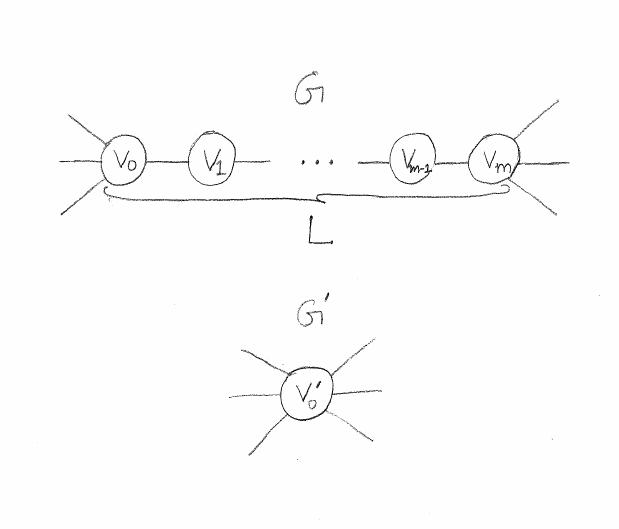
\includegraphics[scale=0.6]{contraction}
\end{figure}
Let $\Phi(G) = \ker \beta/\im \alpha$ and let $\Phi(G') = \ker \beta'/\im \alpha'$ as in Section~\ref{intrograph}. Choose an ordering $(v_0,v_1,\ldots,v_m)$ of $V(L)$ as in the definition of a chain, and let $\{v_0'\}$ be the image of $V(L)$ in $V(G')$. Let $f_0 \colon V(G') \rightarrow V(G)$ be the section of the natural quotient map $V(G) \rightarrow V(G')$ that satisfies $f_0(v_0') = v_0$. Let $f \colon \Z^{V(G')} \rightarrow \Z^{V(G)}$ be the linear map defined by $f_0$ on the corresponding basis elements. We will now define another map $h$ such that the maps in the following diagram commute. 
 \begin{equation*}
 {\xymatrix{
\Z^{V(G')} \ar[dd]_{h} \ar[rr]^{\alpha'} & & \Z^{V(G')} \ar[dd]_{f} \ar[rr]^{\beta'} & & \Z \ar@{=}[dd] \\
& & & & \\
\Z^{V(G)} \ar[rr]^{\alpha} & & \Z^{V(G)} \ar[rr]^{\beta} & & \Z. 
}}
\end{equation*} 
Then $f$ will induce a homomorphism from the homology $\Phi(G')$ of the top row to the homology $\Phi(G)$ of the bottom row. 

We will describe $h$ by giving its value on each $v' \in V(G')$. In order to define $h$, for every $v' \in V(G')$, it suffices to find $v \in \Z^{V(G)}$ (depending on $v'$) such that $\alpha (v) = f(\alpha'(v'))$; we can then define $h(v') = v$. 

{\bf{Case 1:}} $v' \notin \{v_0'\} \cup f_0^{-1}(N_G(v_m))$. \\
In this case, let $h(v') \colonequals f_0(v')$. Since the edges emanating from $v'$ are in bijection with the edges emanating from $f_0(v')$, it follows that $\alpha (f_0(v')) = f(\alpha' (v'))$. 

{\bf{Case 2:}} $v' \in f_0^{-1}(N_G(v_m)) \setminus \{v_0'\}$. \\
In this case $f(\alpha'(v')) = \alpha(f_0(v'))+\Gamma_{v'}.\Gamma_{v_0'}(v_m-v_0)$. It therefore suffices to find $t_1 \in \Z^{V(G)}$ such that $\alpha(t_1) = \Gamma_{v'}.\Gamma_{v_0'}(v_m-v_0)$, since we can then define $h(v') = f_0(v')+t_1$. 

Let $V(G) \setminus V(L) = D_0 \cup D_m$, where $D_0$ (respectively $D_m$) consists of the vertices of $G$ having a path to $L$ meeting $L$ only at $v_0$ (respectively $v_m$). Let $t = mv_m+\sum_{w \in D_m} \beta(w) w$. If $v \notin D_m \cup \{v_{m-1},v_m\}$, then the vertex $v$ has no neighbours in $D_m \cup \{v_m\}$, so the coefficient of $v$ in $\alpha(t)$ is $0$. For any vertex $v$, we have $\alpha(v) = \alpha_{v,v} v + \sum_{w \in N_G(v)} \alpha_{v,w} w$; it follows that if $v \in D_m$, then the coefficient of $v$ in $\alpha(t)$ equals the coefficient of $v$ in $\alpha(\sum_{w \in V(G)} \beta(w) w)$. The latter is $0$ since $\sum_{w \in V(G)} \beta(w) \alpha_{w',w} = 0$ for every $w' \in V(G)$.  By a similar argument, the coefficient of $v_m$ in $\alpha(t+\beta(v_{m-1})v_{m-1})$ is $0$ since it equals the coefficient of $v_m$ in $\alpha(\sum_{w \in V(G)} \beta(w) w)$. The same type of argument also shows that the coefficient of $v_{m-1}$ in $\alpha(t-mv_m)$ is $0$. Since $\beta(v_{m-1}) = \beta(v_m) = m$, we conclude that $\alpha(t) = mv_{m-1}-mv_m$. 

Fix $j$ such that $0 \leq j \leq m-1$. Let $x_j = \sum_{i=1}^j iv_i$. Since $\alpha(v_j) = v_{j-1}-2v_j+v_{j+1}$, an inductive argument shows that $\alpha(x_j) = v_0-(j+1)v_j+jv_{j+1}$. Let $t_1 = -\Gamma_{v'}.\Gamma_{v_0'}(x_{m-1}+t)$. It follows that $\alpha(t_1) = \Gamma_{v'}.\Gamma_{v_0'}(v_m-v_0)$.

{\bf{Case 3:}} $v' = v_0'$. \\
We have $f(\alpha'(v_0')) = \alpha(v_0+v_m)-v_1-v_{m-1}+2v_m$. It therefore suffices to find $t_2 \in \Z^{V(G)}$ such that $\alpha(t_2) = 2v_m-v_1-v_{m-1}$. We may then define $h(v_0') = v_0+v_m+t_2$. 
 
Let $t$ be defined as in Case 2. For $1 \leq j \leq m-1$, let $y_j = \sum_{i=1}^j (i-1)v_i$. Once again an inductive argument as in Case 2 shows that $\alpha(y_j) = v_1-jv_j+(j-1)v_{j+1}$. Let $t_2 = -y_{m-1}-t$. Then $\alpha(t_2) = 2v_m-v_1-v_{m-1}$.

We have now proved that $f$ induces a well-defined map from $\Phi(G')$ to $\Phi(G)$. We want to prove that this map is an isomorphism. Since $|\Phi(G')| = |\Phi(G)|$ (by the proof of Theorem~\ref{uniformbound}), it suffices to prove that it is a surjection. Let $u \in \ker \beta$. We will inductively construct a sequence of elements $u_0,u_1,\ldots,u_m$ such that 
 \begin{itemize}
  \item $u_0 = u$ and $u_m \in \im f$,
  \item For every $i$ satisfying $0 \leq i \leq m-1$, we have $u_{i+1}-u_i \in \im \alpha \subset \ker \beta$. 
  \item For every $i$ satisfying $1 \leq i \leq m$, and for every $j \in \{{m-i+1},{m-i+2},\ldots,m\}$, the coefficient of $v_j$ in $u_i$ is $0$.  
 \end{itemize}
 For the inductive step, suppose that $1 \leq i \leq m-2$ and $u_i = \sum -a_v v$, where $a_v \in \Z$. Let 
 \[ u_{i+1} = u_i + \alpha(a_{v_{m-i}} v_{m-i-1}) = u_i+a_{v_{m-i}}(v_{m-i-2}-2v_{m-i-1}+v_{m-i}) .\] 
 From the equation above, it follows that for $j \in \{m-i+1,m-i+2,\ldots,m \}$ the coefficient of $v_j$ in $u_{i+1}$ is the same as that in $u_i$, and that the coefficient of $v_{m-i}$ in $u_{i+1}$ is $-a_{v_{m-i}}+a_{v_{m-i}} = 0$. The induction hypothesis implies that $a_{v_j} = 0$ for $j \in \{m-i+1,m-i+2,\ldots,m\}$. This finishes the induction. So to finish the construction, it now suffices to prove that $u_m \in \im f$. 
 
 Let $T = V(G) \setminus \{v_1,v_2,\ldots,v_m\}$. By the definition of the map $f$, it maps $\Z^{V(G')}$ isomorphically on to the subset of elements of $\Z^{V(G)}$ supported on $T$. This isomorphism maps $\ker \beta'$ isomorphically to the set of elements of $\ker \beta$ supported on $T$. Since $u_m \in \ker \beta$ and is supported on $T$, this shows that $u_m \in \im f$.  Since $u_m-u_0 \in \im \alpha$, this completes the proof of surjectivity of $f$ on to $\Phi(G)$.   
\end{proof}

\begin{rmk}
 Fix $g$. If $\cha k = 0$, then it is possible to list all the groups that can arise as the component group of the Jacobian of a nice curve of genus $g$ by combining the theorem above with Theorem~\ref{finsim} and Theorem~\ref{typeexistence}.
\end{rmk}

\subsubsection{The N\'{e}ron component series for Jacobians}\label{altprfcomp}
In this section, we provide an alternate proof of \cite[Chapter~3, Proposition~3.1.1]{halnic}, that works in both the equal characteristic and mixed characteristic cases. For the proof, we use the explicit formula in Theorem~\ref{compformula} and the behaviour of {\textup{snc}} models under tame extensions, as described in Section~\ref{deftameext}.

\begin{prop}\cite[Chapter~3, Proposition~3.1.1]{halnic}\label{newproof}
 Let $X$ be the minimal {\textup{snc}} model of a nice $K$-curve of genus $g \geq 1$. Let $d \in \N'$ be an integer prime to $e(X)$. Let $\mathcal{A}$ denote the N\'{e}ron model of the Jacobian of $X_\eta$ and let $\mathcal{A}(d)$ denote the N\'{e}ron model of the Jacobian of $X \times_K K(d)$. Let $t$ denote the toric rank of $\mathcal{A}$. Then
 \[ |\Phi(\mathcal{A}(d))| = d^t |\Phi(\mathcal{A})| .\]
\end{prop}
\begin{proof}
 Let $X(d)$ be the minimal desingularization of the normalization $X_d$ of $X \times_R R(d)$. Let $G$ be the dual graph of $X_s$ and let $G'$ be the dual graph of $X(d)_s$. As mentioned before Proposition~\ref{comodel}, $X(d)$ is a {\textup{snc}} model. Let $J$ be the Jacobian of $X_\eta$.
  
 {\bf{Case 1:}} $J$ is an elliptic curve with multiplicative reduction.\\
  In this case, \cite[Theorem~6.6]{llr} tells us that the minimal {\textup{snc}} model and the minimal regular model coincide, and $X_s$ is also a cycle of rational curves, where the rational curves in the cycle all have the same multiplicity, say $m$. Since the number of spanning trees of $G$ equals the number of vertices in the cycle, and for each spanning tree $T$, the product $\prod_{v \in V(T)} m_v^{N_T(v)-2}$ equals $1/m^2$, the explicit formula in Theorem~\ref{compformula} implies that the order of the component group of the N\'{e}ron model of $J$ equals the number of vertices in the cycle $G$.   
  
  We will first show that $X(d)_s$ is also a cycle of rational curves, and then compute the number of rational curves in the cycle. Formula~\ref{formula} would once again imply that the order of the component group equals the number of vertices in the cycle $G'$.
 
 Proposition~\ref{comodel}(ii) implies that every component of $(X_d)_s$  intersects exactly two other components. Since $(X_d)_s$ is connected by Zariski's connectedness principle, we conclude that it is a cycle of rational curves. Proposition~\ref{comodel}(iii) tells us that in order to obtain $X(d)_s$ from $(X_d)_s$, we have to replace each node in the cycle of rational curves by a chain of rational curves of appropriate length. This implies that $(X_d)_s$ is also a cycle of rational curves. Now,
 \begin{itemize}
  \item Proposition~\ref{comodel}(ii) implies that the number of irreducible components of $(X_d)_s$ equals $\gcd(d,m)$ times the number of irreducible components of $X_s$. 
  \item Proposition\ref{comodel}(iii) and Proposition~\ref{combdata} imply that the preimage of each singular point of $(X_d)_s$ is a chain of rational curves, where the number of rational curves in the chain equals $d/\gcd(d,m)$. 
  \item The number of singular points of $(X_d)_s$ equals the number of irreducible components of $(X_d)_s$. 
 \end{itemize}
 Combining the arguments above, we conclude that the number of irreducible components of $X(d)_s$ is $d$ times the number of irreducible components of $X_s$, and this finishes the proof in this case, since the toric rank $t$ equals $1$.
 
 {\bf{Case 2:}} $J$ is not an elliptic curve with multiplicative reduction. \\
 Then either $g \geq 2$, or $J$ is an elliptic curve with good or additive reduction. Lemma~\ref{dgraphbaseext} implies that $X_s$ and $(X_d)_s$ have the same dual graph. Proposition~\ref{comodel}(iii) implies that $G'$ is a subdivision of $G$. Let $\pi \colon E(G') \rightarrow E(G)$ be the surjective map that maps an edge of $G'$ to the unique edge in $G$ that it is a subdivision of. Let $v$ and $w$ be neighbouring vertices of $G$. In this case, the proof of \cite[Lemma~2.3.2]{halnic} tells us that $\gcd(d,m_v,m_w) = 1$. Let
 \begin{itemize}
  \item $h_v = \gcd(d, m_v)$, 
  \item $h_w = \gcd(d, m_w)$,
  \item $m_v = h_v m_v'$,
  \item $m_w = h_w m_w'$, and,
  \item $d = h_v h_w d'$.
 \end{itemize}
 Then $dm_v' m_w' = d'm_v m_w$. Let $v'$ and $w'$ be the corresponding vertices of $G'$ and let $u_1, u_2, \ldots, u_\lambda$ be the intermediate vertices. Then Lemma~\ref{dgraphbaseext}(ii) tells us that $m_{v'} = m_v'$ and $m_{w'} = m_w'$. Let $r$ be the unique solution to $rm_{v'}+m_{w'} = 0 \mod d'$. Let $(\mu_1,\mu_2, \ldots, \mu_{\lambda})$ be the multiplicity vector associated to the tuple $(d',r,m_{v'},m_{w'})$. By Proposition~\ref{combdata} $m_{u_i} = \mu_i$. By Lemma~\ref{curious},
 \begin{equation}\label{scale}
 \frac{d}{m_v m_w} = \frac{d'}{m_v' m_w'} = \frac{1}{m_v' \mu_1} + \frac{1}{\mu_1 \mu_2} + \cdots + \frac{1}{\mu_{\lambda-1} \mu_\lambda} + \frac{1}{\mu_\lambda m_w'} . 
 \end{equation}
 
 Let $H$ be a connected graph. Let $S(H)$ be the collection of spanning trees of $H$. The first Betti number $t(H)$ of a connected graph $H$ equals $|V(H)|-|E(H)|+1$. Let $T \in S(H)$. Since $|V(H)| = |V(T)|$, and the first Betti number of a tree equals $2$, it follows that $\# (E(H) \setminus E(T)) = t(H)$. For a spanning tree $T$ of a dual graph $H$, let $\phi(T) = \prod_{v \in V(H)} m_v^{N_T(v)-2}$. Fix a dual graph $H$. Let $\delta \colon E(H) \rightarrow \N$ be the map defined by $\delta(e) \colonequals m_v m_w$, where $v$ and $w$ are the endpoints of $e$, and $m_v$ and $m_w$ are the multiplicities of the corresponding irreducible components in the special fiber. 
 
 Fix $T' \in S(G')$. Let $T$ be the subgraph of $G$ such that $V(T) = V(G)$ and such that $E(T) = \{ e \in E(T) \ | \ \pi^{-1}(e) \subset E(T') \}$. Since $G'$ is a subdivision of $G$, it follows that $T$ is a spanning tree of $G$. The construction $T' \mapsto T$ defines a map $\tau \colon S(G') \rightarrow S(G)$. Let $T' \in S(B')$ and let $\tau(T') = T$. Let $B' = E(G') \setminus E(T')$ and let  $B = E(G) \setminus E(T)$. Let $\pi_T$ be the restriction of $\pi$ to $\pi^{-1}(B)$. Let $\epsilon \colon \pi^{-1}(B) \rightarrow \Q^\times$ be the map defined by $\epsilon(e) = \delta(\pi(e))/\delta(e)$. Since $G'$ is a subdivision of $G$, it follows that
 \begin{itemize}
  \item $t(G') = t(G)$, and,
  \item there is a multiplicity-preserving bijection between the vertices of $T'$ of degree $\geq 3$ and those of $T$ of degree $\geq 3$.
 \end{itemize}
The two facts above imply that 
\[ \phi(T')/\phi(T) = \prod_{e \in B'} \epsilon(e) .\]
Since $G'$ is a subdivision of $G$, it follows that there exists a bijection
\[ \{ T'' \in S(G') \ | \ \tau(T'') = T \} \longleftrightarrow \textup{Sections } \sigma \colon B \rightarrow \pi^{-1}(B) \textup{ of } \pi_T .\]
Let $\mathfrak{s}$ denote the set of sections of $\pi_T$. Since $t(G) = t(G')$, and the toric rank $t$ equals the first Betti number of the graphs $G$ and $G'$ (by \cite[9.2.5,9.2.8]{blr}), it follows that $\# B = \# B' = t$. Now
\begin{align*} \sum_{T' \in \tau^{-1}(T)} \frac{\phi(T')}{\phi(T)} &= \sum_{\sigma \in \mathfrak{s}} \prod_{e \in B} \epsilon (\sigma(e)) \\
&= \prod_{e \in B} \sum_{e' \in \pi^{-1}(e)} \epsilon(e') \\
&= \prod_{e \in B} \delta(e) \sum_{e' \in \pi^{-1}(e)} \frac{1}{\delta(e')} \\
&= \prod_{e \in B} \delta(e) \frac{d}{\delta(e)} \ \ \ (\textup{by Equation~\eqref{scale}}) \\
&= d^{\# B} = d^t.
\end{align*}
Now
\[ \sum_{T' \in S(G')} \phi(T') = \sum_{T \in S(G)} \sum_{T' \in \tau^{-1}(T)} \phi(T') = d^t \sum_{T \in S(G)} \phi(T)  .\]
To finish the proof, it suffices to prove that $\gcd(m_v \ | \ v \in V(G)) = \gcd(m_{v'} \ | \ v' \in V(G'))$ by the formula in Theorem~\ref{compformula}. Lemma~\ref{gcdmult} implies that the gcd of the multiplicities of the components of $X_d$ and the gcd of the multiplicities of the components of $X(d)$ are equal. This implies that it now suffices to prove $\gcd(m_v \ | \ v \in V(G)) = \gcd(m_v/\gcd(m_v,d) \ | \ v \in V(G))$. The right hand side divides the left hand side. To prove the other divisibility, we use the fact that $G$ is connected, and the fact that if $v$ and $w$ are any pair of neighbouring vertices in $G$, then $\gcd(m_v,m_w,d) = 1$ (this follows from the proof of Lemma~\ref{dgraphbaseext} in \cite{halnic}). This concludes the proof. \qedhere
\end{proof}

\section{Explicit computation of Tamagawa numbers}\label{tamagawa}
%Let $C$ be a nice curve over $K$ and let $X$ be a regular model for $C$ over $R$. The component group $\Phi$ which was defined in Section~\ref{compgroup} is in fact the set of $\overline{k}$ points of a finite \'{e}tale $k$-group scheme $\phi$, called the component group scheme. The order of the set of $k$ points of this scheme is the Tamagawa number associated to the curve $C$. 

In this section, we will show that we can use a version of the matrix-tree theorem for directed weighted multigraphs to compute Tamagawa numbers. The notation used in this section is consistent with the notation in Section~\ref{introtam}. 

% In this section, we do not assume that the residue field $k$ is algebraically closed. We assume that $k$ is perfect and we let $\overline{k}$ denote an algebraic closure of $k$. Let $R^{\textup{st}}$ denote the strict henselization of $R$. Let $X$ be a regular $S$-curve. 

\subsection{The quotient graph $\widetilde{G}$}
Let $X^{\textup{st}} = X \times_R R^{\textup{st}}$. Let $G$ denote the dual graph of $X^{\textup{st}}_s$, and let $V = V(G)$. We now define a directed weighted multigraph $\widetilde{G}$, which we call the quotient graph. The set of vertices of $\widetilde{G}$, which we denote $\widetilde{V}$, is the the set of irreducible components of $X_s$. The set $\widetilde{V}$ can also naturally be identified with the set of orbits of $V$ under the natural action of $\Gal (\overline{k}/k)$. This identification gives rise to a quotient map $\pi \colon V \rightarrow \widetilde{V}$ where we map a vertex $v$ to the corresponding orbit. For any two vertices $\tilde{w}$ and $\tilde{v}$ in $\widetilde{V}$, the number of directed edges with tail $\tilde{w}$ and head $\tilde{v}$, which we denote $\alpha_{\tilde{w} \tilde{v}}$, is defined as follows. Fix any $w \in \pi^{-1}(\tilde{w})$.  Then $\alpha_{\tilde{w} \tilde{v}} = \sum_{v \in \pi^{-1}(\tilde{v})} \Gamma_v.\Gamma_w$. Since the Galois action transitively permutes the 
vertices $w \in \pi^{-1}(\tilde{w})$ and preserves intersection numbers, the sum is independent of the choice of $w \in \pi^{-1}(\tilde{w})$. This defines the vertices and directed edges of $\widetilde{G}$.

We now define a weight function on $\widetilde{G}$. For every $\tilde{v} \in \widetilde{V}$, let $|\tilde{v}|$ denote the size of the orbit corresponding to $\tilde{v}$. For any $\tilde{v} \in \widetilde{V}$, let $\Gamma_{\tilde{v}}$ denote the corresponding irreducible component of $X_s$, and let $m_{\tilde{v}}$ denote the multiplicity of $\Gamma_{\tilde{v}}$ in the special fiber $X_s$. For any directed edge $e$ with tail $\tilde{w}$ and head $\tilde{v}$, the weight of the edge $e$, denoted $\wt(e)$ is defined to be $m_{\tilde{v}} m_{\tilde{w}} |\tilde{w}|$. 

\subsection{Explicit computation of Tamagawa numbers}
In this section, we will show how to combine Theorem~\ref{galcoh} and Theorem~\ref{matrixtree} to explicitly compute Tamagawa numbers. In the rest of this section, we will assume that $\Gal (\overline{k}/k)$ is procyclic in order to be able to apply Theorem~\ref{galcoh}.

\begin{rmk}
The order of the component group can also be computed using using Theorem~\ref{matrixtree} (this corresponds to the special case where $k = \overline{k}$). The formula that we obtain for the component group using Theorem~\ref{matrixtree} can be checked to be equal to the formula obtained in Theorem~\ref{compformula}. We included the proof in Section~\ref{compgroup} since the graph that appears in Section~\ref{compgroup} is more closely related to the dual graph that appears in algebraic geometry.
\end{rmk}

Let $\alpha$ and $\beta$ be as in Section~\ref{introtam}. We now show that if we make the appropriate modifications to $\alpha$ and $\beta$, we can use Theorem~\ref{matrixtree} to compute Tamagawa numbers. Define maps $\delta_1, \delta_2, \alpha_1,\beta_1,\beta_2$ as follows:
\begin{align*}
 \delta_1 \colon \Z^{\widetilde{V}} &\rightarrow \Z^{\widetilde{V}} \\
 (b_{\tilde{v}}) &\mapsto (b_{\tilde{v}}m_{\tilde{v}}|\tilde{v}|) \\
 \delta_2 \colon \Z^{\widetilde{V}} &\rightarrow \Z^{\widetilde{V}} \\
 (b_{\tilde{v}}) &\mapsto (b_{\tilde{v}}m_{\tilde{v}}) \\
\alpha_1 = \delta_1 &\circ \alpha \circ \delta_2 \\
\beta_1 \colon \Z^{\widetilde{V}} &\rightarrow \Z \\
 (b_{\tilde{v}}) &\mapsto \sum_{\tilde{v} \in \widetilde{V}} b_{\tilde{v}} \\
\beta_2 \colon \Z &\rightarrow \Z^{\widetilde{V}} \\
 b &\mapsto (b,b,\ldots,b)  .
\end{align*}
We have $\beta_1 \delta_1 = \beta$, so $\beta_1 \alpha_1 = \beta_1 \delta_1 \alpha \delta_2 = \beta \alpha \delta_2 = 0$. This implies that $\im(\alpha_1) \subset \ker{\beta_1}$.

We now prove a lemma in linear algebra that allows us to compare the orders of the finite groups $\ker(\beta_1)/\im(\alpha_1)$ and $\ker(\beta)/\im(\alpha)$.
\begin{lemma}\label{linear}
Let $n$ be a nonnegative integer. Let $D, D' \colon \Z^n \rightarrow \Z^n$ be two rank $n$ linear operators whose matrices are diagonal. Let $A \colon \Z^n \rightarrow \Z^n$ be a rank $n-1$ linear operator. Let $S \colon \Z^n \rightarrow \Z$ denote the linear operator which takes a vector to the sum of its coordinates, and let $\Delta \colon \Z \rightarrow \Z^n$ denote the diagonal embedding. Assume $SDA = 0$ and $AD'\Delta = 0$. Let $d,d'$ be positive integers such that $d\Z = \im \left( SD \right)$ and $d'\Z = \im \left( SD' \right)$ respectively. Then
\begin{equation}\label{lalg} \# \frac{\ker (S D) }{\im A} = \frac{d}{|\det D|} \cdot \# \frac{\ker S }{\im (D A)} = \frac{dd'}{|\det D| |\det D'|} \cdot \# \frac{\ker S }{\im ( D A D' )} .\end{equation}
\end{lemma}
\begin{proof}
 The integer $d$ is the gcd of the diagonal entries of $D$. Thus $\tfrac{1}{d} D \in M_n(\Z)$. Similarly $\tfrac{1}{d'} D' \in M_n(\Z)$. Replacing $D$ by $\tfrac{1}{d}D$ and replacing $D'$ by $\tfrac{1}{d'}D'$ multiplies the five ratios in Equation~\eqref{lalg} by $1,d^{n-1},d^{1-n},(dd')^{n-1}$ and $(dd')^{1-n}$ respectively. Therefore we may assume $d=d'=1$ without any loss of generality.
 
We now prove the first equality. For this, we show that the following sequence is exact.
\[ 0 \rightarrow \frac{\ker (SD)}{\im A} \xrightarrow{D} \frac{\ker S}{\im (DA)} \rightarrow \frac{\Z^n}{\im D}  \rightarrow 0 . \]
The exactness at the left follows because $D$ is an injection, and therefore restricts to an injection from $\ker (SD)$ to $\ker S$, and also implies that $D^{-1} (\im (DA)) = \im A$. The exactness at the middle follows because $D(\ker (SD)) = \ker S \cap \im D$. For the exactness on the right, it suffices to show that $\Z^n/(\ker S + \im D) = 0$. This follows because $\Z^n/(\ker S + \im D) \simeq \im S/\im(SD) = \Z/d\Z = 0$, since $d=1$. Since all the groups in the above exact sequence are finite and $\# \left( \tfrac{\Z^n}{\im D} \right) = |\det D|$, we get 
\[ \# \frac{\ker (S D) }{\im A} |\det D| =  \# \frac{\ker S }{\im (D A)} .\]
This finishes the proof of the first equality.

Let $A' = DA$. For the second equality, we show that the following sequence is exact.
\[ 0 \rightarrow \frac{\Z^n}{\im D'} \xrightarrow{A'} \frac{\ker S}{\im (A'D')} \rightarrow \frac{\ker S}{\im A'} \rightarrow 0  .\]
First, since $SA' = SDA = 0$, the map on the left is well-defined. Since $d'=1$, it follows that $\im D'\Delta$ is a rank $1$ lattice generated by a primitive vector, and therefore is a saturated submodule of $\Z^n$. On the other hand, we have $\im D' \Delta \subset \ker A'$ (since $A'D'\Delta = DAD'\Delta = 0$), and $\ker A'$ is also a rank $1$ lattice (since $D'$ is injective and $A$ has rank $n-1$). Therefore we must have $\im D' \Delta = \ker A'$, which implies that $\ker A' \subset \im D'$. This in turn implies that $A'^{-1}(\im A'D') = \im D' + \ker A' = \im D'$. This proves exactness on the left of the sequence above. The exactness at the other two positions is immediate.
\end{proof}

\begin{lemma}\label{compare}
Let $m$ and $\tilde{m}$ be as defined as in Theorem~\ref{galcoh}. 
\[ \# \left( \frac{\ker{\beta}}{\im{\alpha}} \right)  = \frac{m \tilde{m}}{\prod_{\tilde{v} \in \widetilde{V}} m_{\tilde{v}}^2 |\tilde{v}| } \ \# \left( \frac{\ker{\beta_1}}{\im{\alpha_1}} \right) .\] 
\end{lemma}
\begin{proof}
This follows directly from Lemma~\ref{linear} with $A = \alpha, D = \delta_1$ and $D' = \delta_2$. \qedhere
\end{proof}

We will now show how we can use Theorem~\ref{matrixtree} to compute $\# (\ker{\beta_1}/\im \alpha_1)$. Recall the definition of the graph $\tilde{G}$ as defined in the beginning of this section.
\begin{lemma}\label{applyingmt}
 Fix a vertex $\tilde{w}$ of the directed weighted multigraph $\widetilde{G}$. Let $\widetilde{S}_{\tilde{w}}(\widetilde{G})$ be the set of directed spanning trees into the vertex $\tilde{v}$. Then
 \[ \# \left( \frac{\ker{\beta_1}}{\im{\alpha_1}} \right) = \sum_{T \in \widetilde{S}_{\tilde{w}}(\widetilde{G})} \prod_{e \in E(T)} \wt(e)  .\]
\end{lemma}
\begin{proof}
 We observe that $\# \left( \tfrac{\ker{\beta_1}}{\im{\alpha_1}} \right)$ is equal to the absolute value of the determinant of the reduced Laplacian operator on $\widetilde{G}$, with the fixed vertex $\tilde{w}$ as the sink (since $X_s$ is connected, every vertex of $\widetilde{G}$ is a sink). The determinant can then by computed using Theorem~\ref{matrixtree}.
\end{proof}

\begin{thm}\label{tamnum}
Let $q, m$ and $\tilde{m}$ be defined as in Theorem~\ref{galcoh}.
\begin{equation*}
 \# \Phi(k) = \frac{\tilde{m}^2}{q\prod_{\tilde{v} \in \widetilde{V}} m_{\tilde{v}}^2 |\tilde{v}|} \ \left( \sum_{T \in \widetilde{S}_{\tilde{w}}(\widetilde{G})} \prod_{e \in E(T)} \wt(e) \right)   .
\end{equation*} 
\end{thm}
\begin{proof}
 Combine Theorem~\ref{galcoh}, Lemma~\ref{compare} and Lemma~\ref{applyingmt}.
\end{proof}
\appendix
%\chapter{Tables}

\begin{table}
\caption{Armadillos}
\label{arm:table}
\begin{center}
\begin{tabular}{||l|l||}\hline
Armadillos & are \\\hline
our	   & friends \\\hline
\end{tabular}
\end{center}
\end{table}

\clearpage
\newpage

%\chapter{Figures}

\vspace*{-3in}

\begin{figure}
\vspace{2.4in}
\caption{Armadillo slaying lawyer.}
\label{arm:fig1}
\end{figure}
\clearpage
\newpage

\begin{figure}
\vspace{2.4in}
\caption{Armadillo eradicating national debt.}
\label{arm:fig2}
\end{figure}
\clearpage
\newpage

%% This defines the bibliography file (main.bib) and the bibliography style.
%% If you want to create a bibliography file by hand, change the contents of
%% this file to a `thebibliography' environment.  For more information 
%% see section 4.3 of the LaTeX manual.
\begin{singlespace}
\bibliography{main}
\bibliographystyle{plain}
\end{singlespace}

\end{document}

